\batchmode
\documentclass{book}
\RequirePackage{ifthen}


\usepackage{color,epsfig,makeidx,moreverb}
\usepackage{times}

\hyphenation{white-space} 
\definecolor{lightblue}{rgb}{.5,.5,1}
\makeindex
\pagenumbering{roman}
\paperwidth 8.5in
\paperheight 11in



\pagecolor[gray]{1.0}

\usepackage[latin1]{inputenc}



\makeatletter
\AtBeginDocument{\makeatletter
\input /home/george/plt-2.4/doc/book.aux
\makeatother
}

\makeatletter
\count@=\the\catcode`\_ \catcode`\_=8 
\newenvironment{tex2html_wrap}{}{}%
\catcode`\<=12\catcode`\_=\count@
\newcommand{\providedcommand}[1]{\expandafter\providecommand\csname #1\endcsname}%
\newcommand{\renewedcommand}[1]{\expandafter\providecommand\csname #1\endcsname{}%
  \expandafter\renewcommand\csname #1\endcsname}%
\newcommand{\newedenvironment}[1]{\newenvironment{#1}{}{}\renewenvironment{#1}}%
\let\newedcommand\renewedcommand
\let\renewedenvironment\newedenvironment
\makeatother
\let\mathon=$
\let\mathoff=$
\ifx\AtBeginDocument\undefined \newcommand{\AtBeginDocument}[1]{}\fi
\newbox\sizebox
\setlength{\hoffset}{0pt}\setlength{\voffset}{0pt}
\addtolength{\textheight}{\footskip}\setlength{\footskip}{0pt}
\addtolength{\textheight}{\topmargin}\setlength{\topmargin}{0pt}
\addtolength{\textheight}{\headheight}\setlength{\headheight}{0pt}
\addtolength{\textheight}{\headsep}\setlength{\headsep}{0pt}
\setlength{\textwidth}{698pt}
\setlength{\textheight}{902pt}
\newwrite\lthtmlwrite
\makeatletter
\let\realnormalsize=\normalsize
\global\topskip=2sp
\def\preveqno{}\let\real@float=\@float \let\realend@float=\end@float
\def\@float{\let\@savefreelist\@freelist\real@float}
\def\liih@math{\ifmmode$\else\bad@math\fi}
\def\end@float{\realend@float\global\let\@freelist\@savefreelist}
\let\real@dbflt=\@dbflt \let\end@dblfloat=\end@float
\let\@largefloatcheck=\relax
\let\if@boxedmulticols=\iftrue
\def\@dbflt{\let\@savefreelist\@freelist\real@dbflt}
\def\adjustnormalsize{\def\normalsize{\mathsurround=0pt \realnormalsize
 \parindent=0pt\abovedisplayskip=0pt\belowdisplayskip=0pt}%
 \def\phantompar{\csname par\endcsname}\normalsize}%
\def\lthtmltypeout#1{{\let\protect\string \immediate\write\lthtmlwrite{#1}}}%
\newcommand\lthtmlhboxmathA{\adjustnormalsize\setbox\sizebox=\hbox\bgroup\kern.05em }%
\newcommand\lthtmlhboxmathB{\adjustnormalsize\setbox\sizebox=\hbox to\hsize\bgroup\hfill }%
\newcommand\lthtmlvboxmathA{\adjustnormalsize\setbox\sizebox=\vbox\bgroup %
 \let\ifinner=\iffalse \let\)\liih@math }%
\newcommand\lthtmlboxmathZ{\@next\next\@currlist{}{\def\next{\voidb@x}}%
 \expandafter\box\next\egroup}%
\newcommand\lthtmlmathtype[1]{\gdef\lthtmlmathenv{#1}}%
\newcommand\lthtmllogmath{\lthtmltypeout{l2hSize %
:\lthtmlmathenv:\the\ht\sizebox::\the\dp\sizebox::\the\wd\sizebox.\preveqno}}%
\newcommand\lthtmlfigureA[1]{\let\@savefreelist\@freelist
       \lthtmlmathtype{#1}\lthtmlvboxmathA}%
\newcommand\lthtmlpictureA{\bgroup\catcode`\_=8 \lthtmlpictureB}%
\newcommand\lthtmlpictureB[1]{\lthtmlmathtype{#1}\egroup
       \let\@savefreelist\@freelist \lthtmlhboxmathB}%
\newcommand\lthtmlpictureZ[1]{\hfill\lthtmlfigureZ}%
\newcommand\lthtmlfigureZ{\lthtmlboxmathZ\lthtmllogmath\copy\sizebox
       \global\let\@freelist\@savefreelist}%
\newcommand\lthtmldisplayA{\bgroup\catcode`\_=8 \lthtmldisplayAi}%
\newcommand\lthtmldisplayAi[1]{\lthtmlmathtype{#1}\egroup\lthtmlvboxmathA}%
\newcommand\lthtmldisplayB[1]{\edef\preveqno{(\theequation)}%
  \lthtmldisplayA{#1}\let\@eqnnum\relax}%
\newcommand\lthtmldisplayZ{\lthtmlboxmathZ\lthtmllogmath\lthtmlsetmath}%
\newcommand\lthtmlinlinemathA{\bgroup\catcode`\_=8 \lthtmlinlinemathB}
\newcommand\lthtmlinlinemathB[1]{\lthtmlmathtype{#1}\egroup\lthtmlhboxmathA
  \vrule height1.5ex width0pt }%
\newcommand\lthtmlinlineA{\bgroup\catcode`\_=8 \lthtmlinlineB}%
\newcommand\lthtmlinlineB[1]{\lthtmlmathtype{#1}\egroup\lthtmlhboxmathA}%
\newcommand\lthtmlinlineZ{\egroup\expandafter\ifdim\dp\sizebox>0pt %
  \expandafter\centerinlinemath\fi\lthtmllogmath\lthtmlsetinline}
\newcommand\lthtmlinlinemathZ{\egroup\expandafter\ifdim\dp\sizebox>0pt %
  \expandafter\centerinlinemath\fi\lthtmllogmath\lthtmlsetmath}
\newcommand\lthtmlindisplaymathZ{\egroup %
  \centerinlinemath\lthtmllogmath\lthtmlsetmath}
\def\lthtmlsetinline{\hbox{\vrule width.1em \vtop{\vbox{%
  \kern.1em\copy\sizebox}\ifdim\dp\sizebox>0pt\kern.1em\else\kern.3pt\fi
  \ifdim\hsize>\wd\sizebox \hrule depth1pt\fi}}}
\def\lthtmlsetmath{\hbox{\vrule width.1em\kern-.05em\vtop{\vbox{%
  \kern.1em\kern1 pt\hbox{\hglue.17em\copy\sizebox\hglue1 pt}}\kern.3pt%
  \ifdim\dp\sizebox>0pt\kern.1em\fi \kern1 pt%
  \ifdim\hsize>\wd\sizebox \hrule depth1pt\fi}}}
\def\centerinlinemath{%
  \dimen1=\ifdim\ht\sizebox<\dp\sizebox \dp\sizebox\else\ht\sizebox\fi
  \advance\dimen1by.5pt \vrule width0pt height\dimen1 depth\dimen1 
 \dp\sizebox=\dimen1\ht\sizebox=\dimen1\relax}

\def\lthtmlcheckvsize{\ifdim\ht\sizebox<\vsize 
  \ifdim\wd\sizebox<\hsize\expandafter\hfill\fi \expandafter\vfill
  \else\expandafter\vss\fi}%
\providecommand{\selectlanguage}[1]{}%
\makeatletter \tracingstats = 1 


\begin{document}
\pagestyle{empty}\thispagestyle{empty}\lthtmltypeout{}%
\lthtmltypeout{latex2htmlLength hsize=\the\hsize}\lthtmltypeout{}%
\lthtmltypeout{latex2htmlLength vsize=\the\vsize}\lthtmltypeout{}%
\lthtmltypeout{latex2htmlLength hoffset=\the\hoffset}\lthtmltypeout{}%
\lthtmltypeout{latex2htmlLength voffset=\the\voffset}\lthtmltypeout{}%
\lthtmltypeout{latex2htmlLength topmargin=\the\topmargin}\lthtmltypeout{}%
\lthtmltypeout{latex2htmlLength topskip=\the\topskip}\lthtmltypeout{}%
\lthtmltypeout{latex2htmlLength headheight=\the\headheight}\lthtmltypeout{}%
\lthtmltypeout{latex2htmlLength headsep=\the\headsep}\lthtmltypeout{}%
\lthtmltypeout{latex2htmlLength parskip=\the\parskip}\lthtmltypeout{}%
\lthtmltypeout{latex2htmlLength oddsidemargin=\the\oddsidemargin}\lthtmltypeout{}%
\makeatletter
\if@twoside\lthtmltypeout{latex2htmlLength evensidemargin=\the\evensidemargin}%
\else\lthtmltypeout{latex2htmlLength evensidemargin=\the\oddsidemargin}\fi%
\lthtmltypeout{}%
\makeatother
\setcounter{page}{1}
\onecolumn

% !!! IMAGES START HERE !!!

{\newpage\clearpage
\lthtmlpictureA{tex2html_wrap3999}%
\epsfig{file=figure10,height=2cm}%
\lthtmlpictureZ
\lthtmlcheckvsize\clearpage}

{\newpage\clearpage
\lthtmlpictureA{tex2html_wrap4001}%
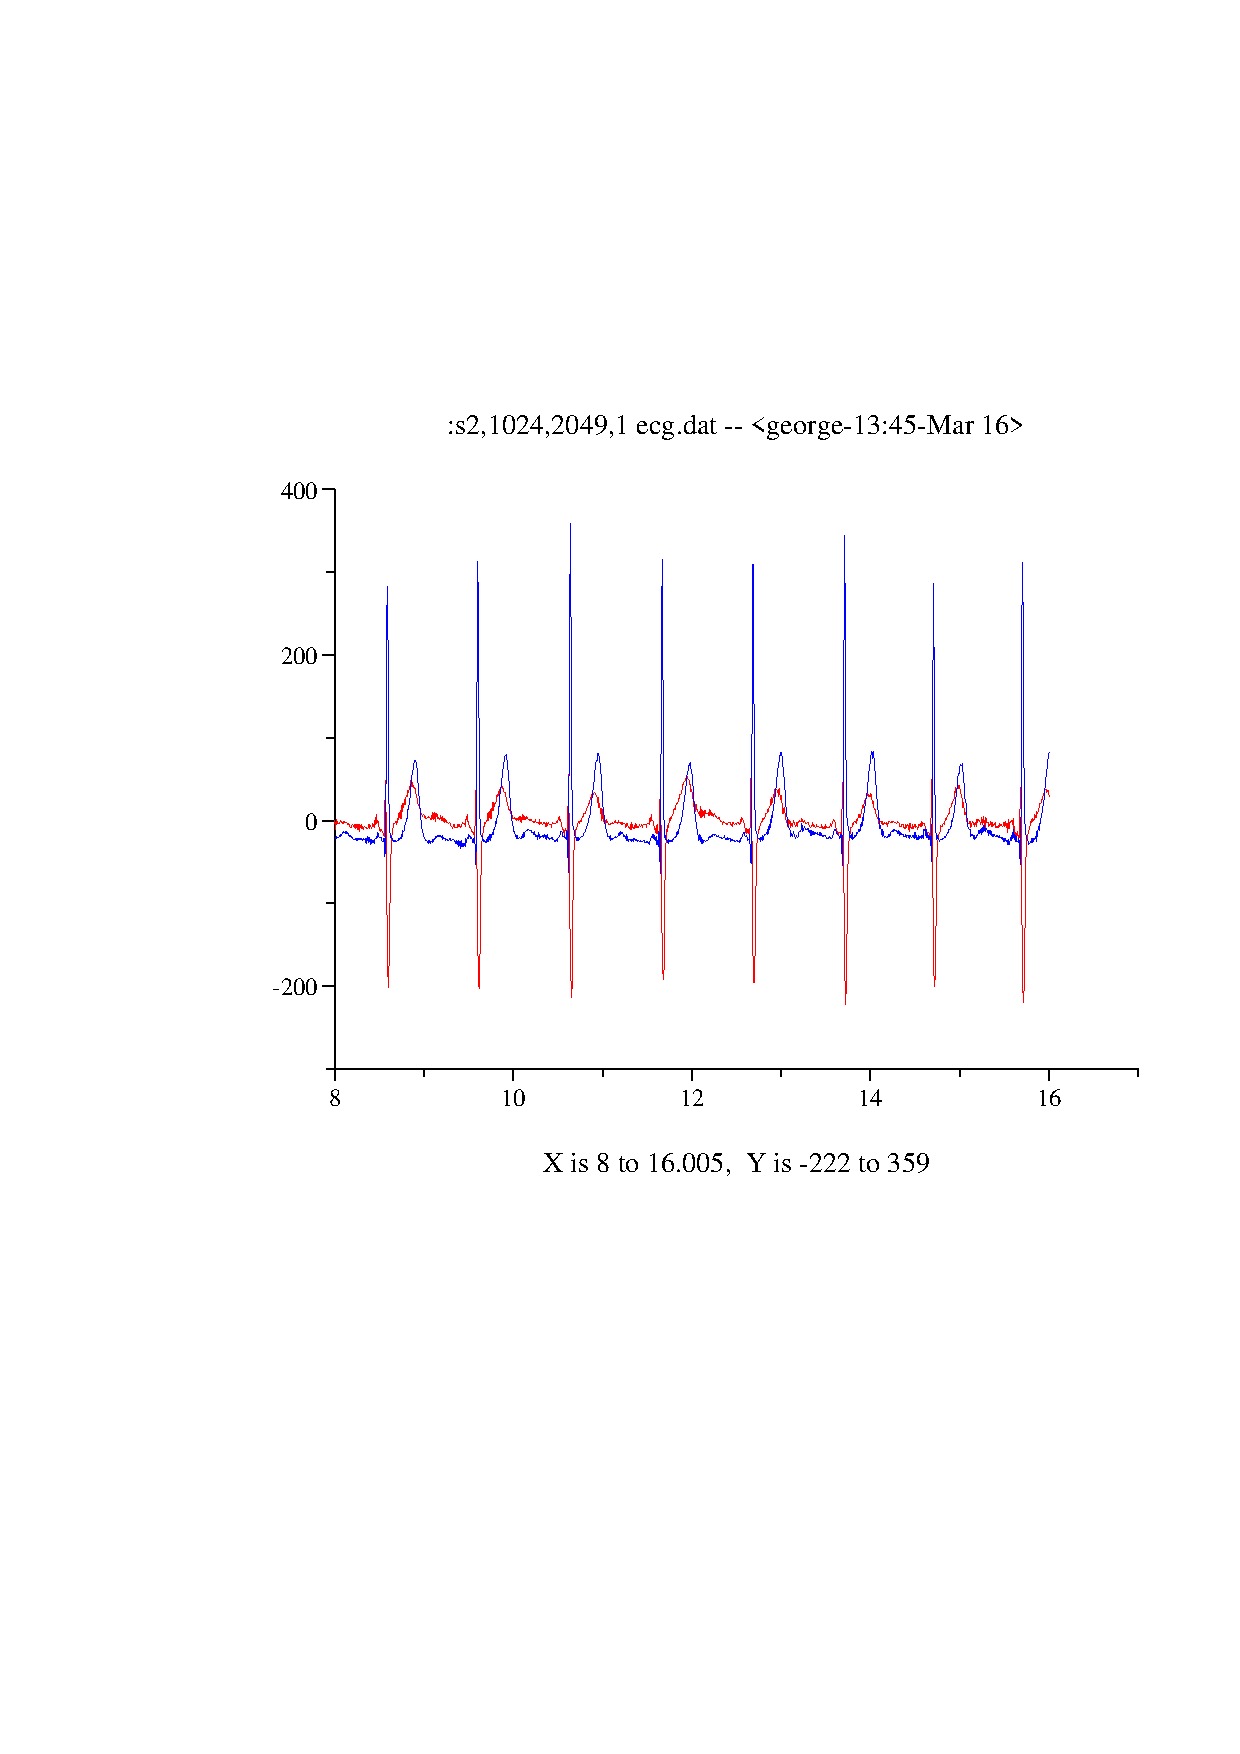
\epsfig{file=ecg,height=2cm}%
\lthtmlpictureZ
\lthtmlcheckvsize\clearpage}

{\newpage\clearpage
\lthtmlpictureA{tex2html_wrap4003}%
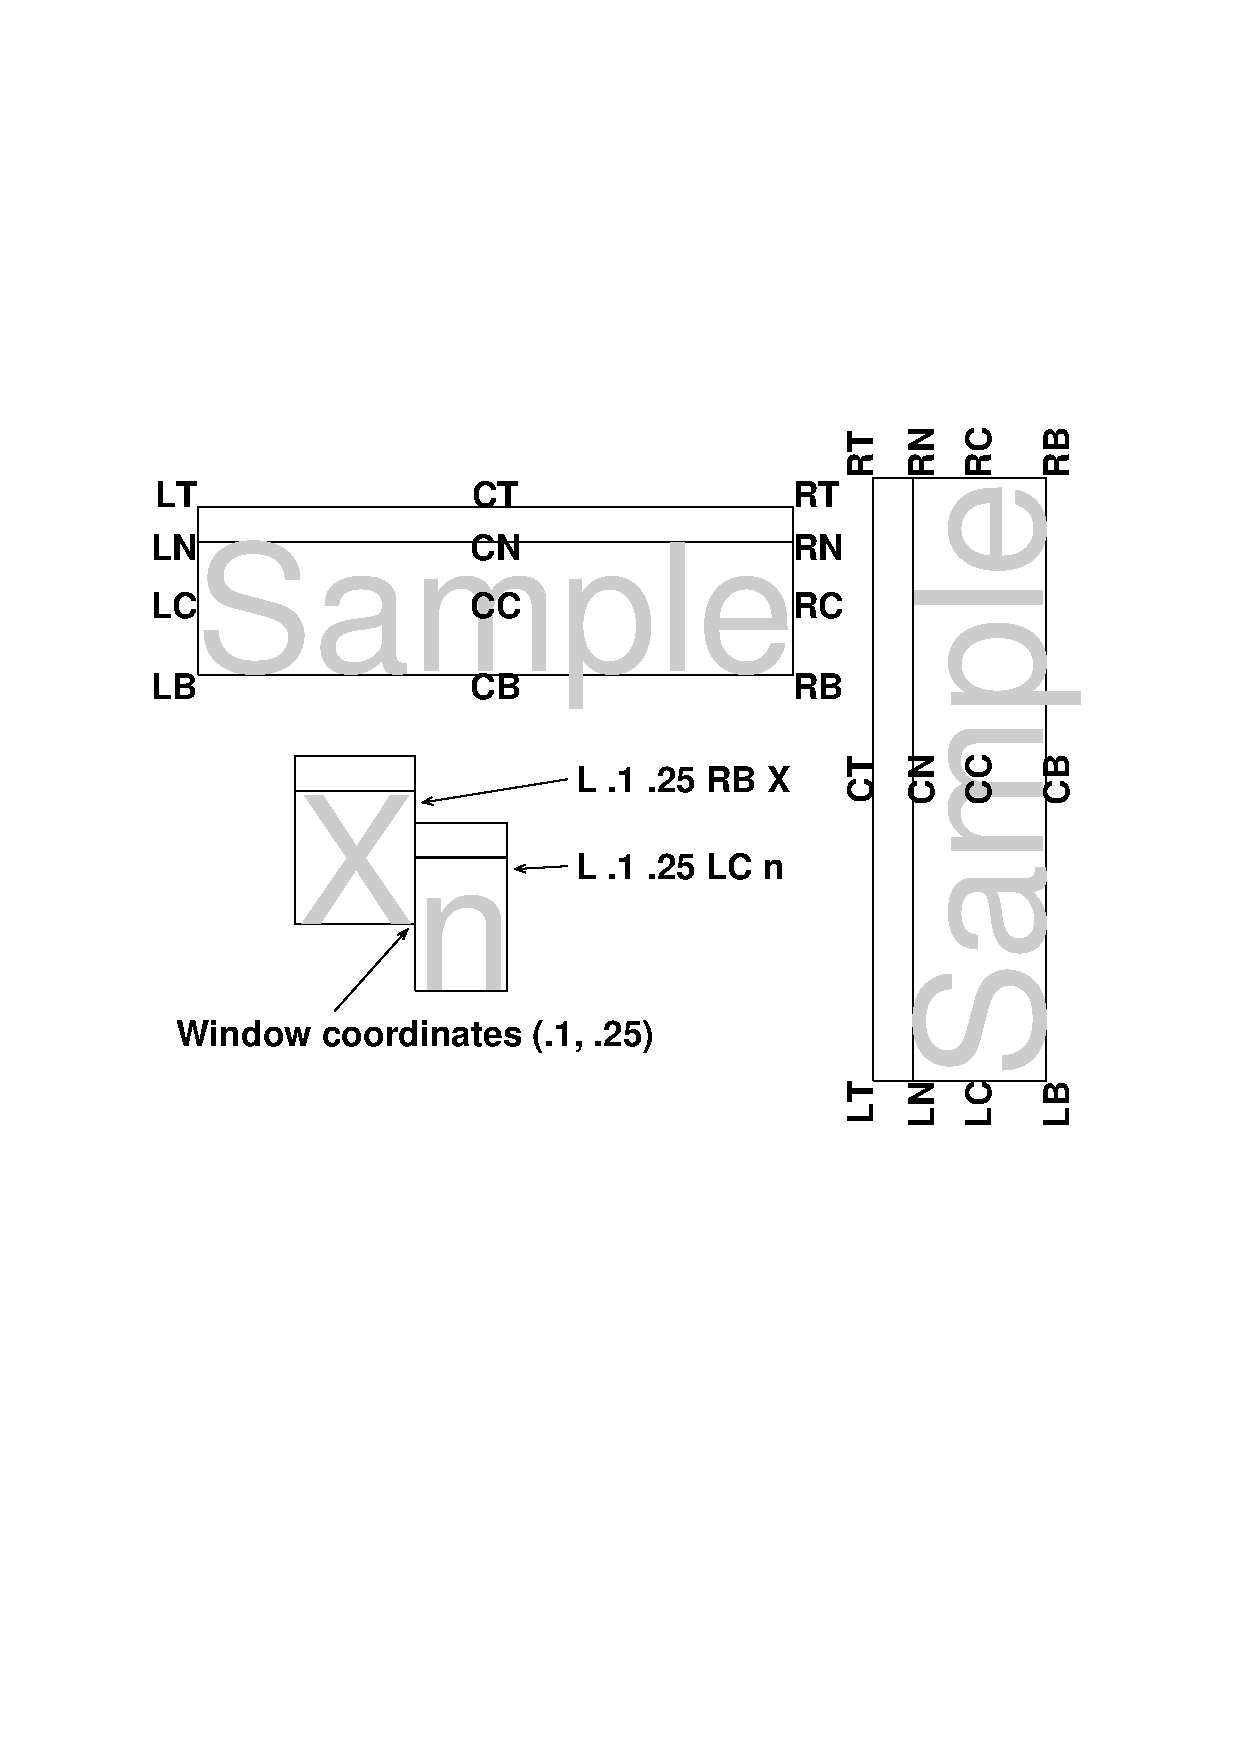
\epsfig{file=figure8,height=2cm}%
\lthtmlpictureZ
\lthtmlcheckvsize\clearpage}

{\newpage\clearpage
\lthtmlpictureA{tex2html_wrap4005}%
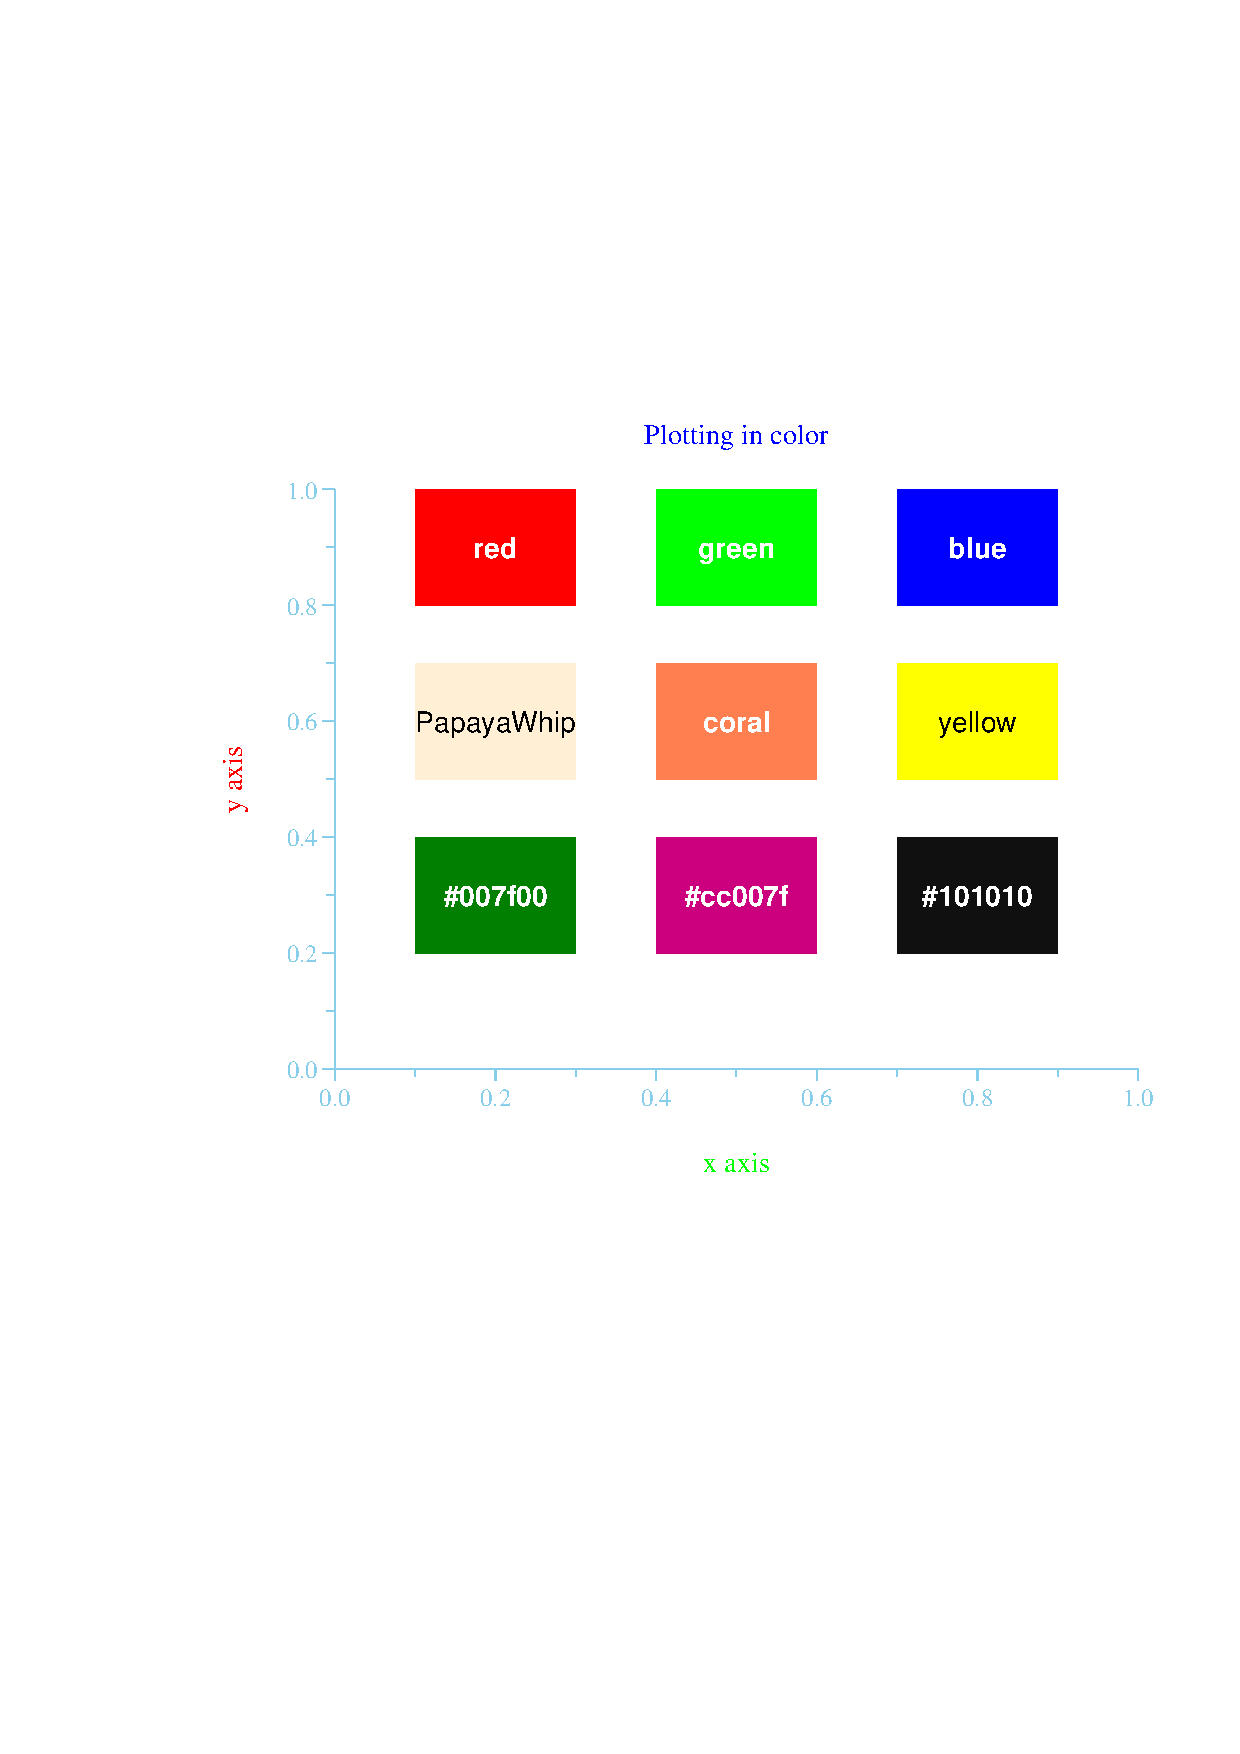
\epsfig{file=colors,height=2cm}%
\lthtmlpictureZ
\lthtmlcheckvsize\clearpage}

{\newpage\clearpage
\lthtmlpictureA{tex2html_wrap4007}%
\epsfig{file=figure14,height=2cm}%
\lthtmlpictureZ
\lthtmlcheckvsize\clearpage}

{\newpage\clearpage
\lthtmlinlinemathA{tex2html_wrap_inline3577}%
$n^{th}$%
\lthtmlinlinemathZ
\lthtmlcheckvsize\clearpage}

\stepcounter{chapter}
\stepcounter{section}
\stepcounter{section}
\stepcounter{section}
\stepcounter{chapter}
\stepcounter{section}
{\newpage\clearpage
\lthtmlinlinemathA{tex2html_wrap_inline4315}%
\fbox{{\tt plt} {\em data-spec data-file column-number ... options}}%
\lthtmlinlinemathZ
\lthtmlcheckvsize\clearpage}

{\newpage\clearpage
\lthtmlinlinemathA{tex2html_wrap_inline3579}%
$\ge 0$%
\lthtmlinlinemathZ
\lthtmlcheckvsize\clearpage}

\stepcounter{section}
{\newpage\clearpage
\lthtmlinlinemathA{tex2html_wrap_inline3581}%
$>$%
\lthtmlinlinemathZ
\lthtmlcheckvsize\clearpage}

{\newpage\clearpage
\lthtmlinlinemathA{tex2html_wrap_inline3583}%
$<$%
\lthtmlinlinemathZ
\lthtmlcheckvsize\clearpage}

\stepcounter{section}
{\newpage\clearpage
\lthtmlfigureA{figure373}%
\begin{figure}
% latex2html id marker 373
\begin{center}
\begin{tabular}{p{10cm}p{1.5cm}}
\fcolorbox{blue}{white}{
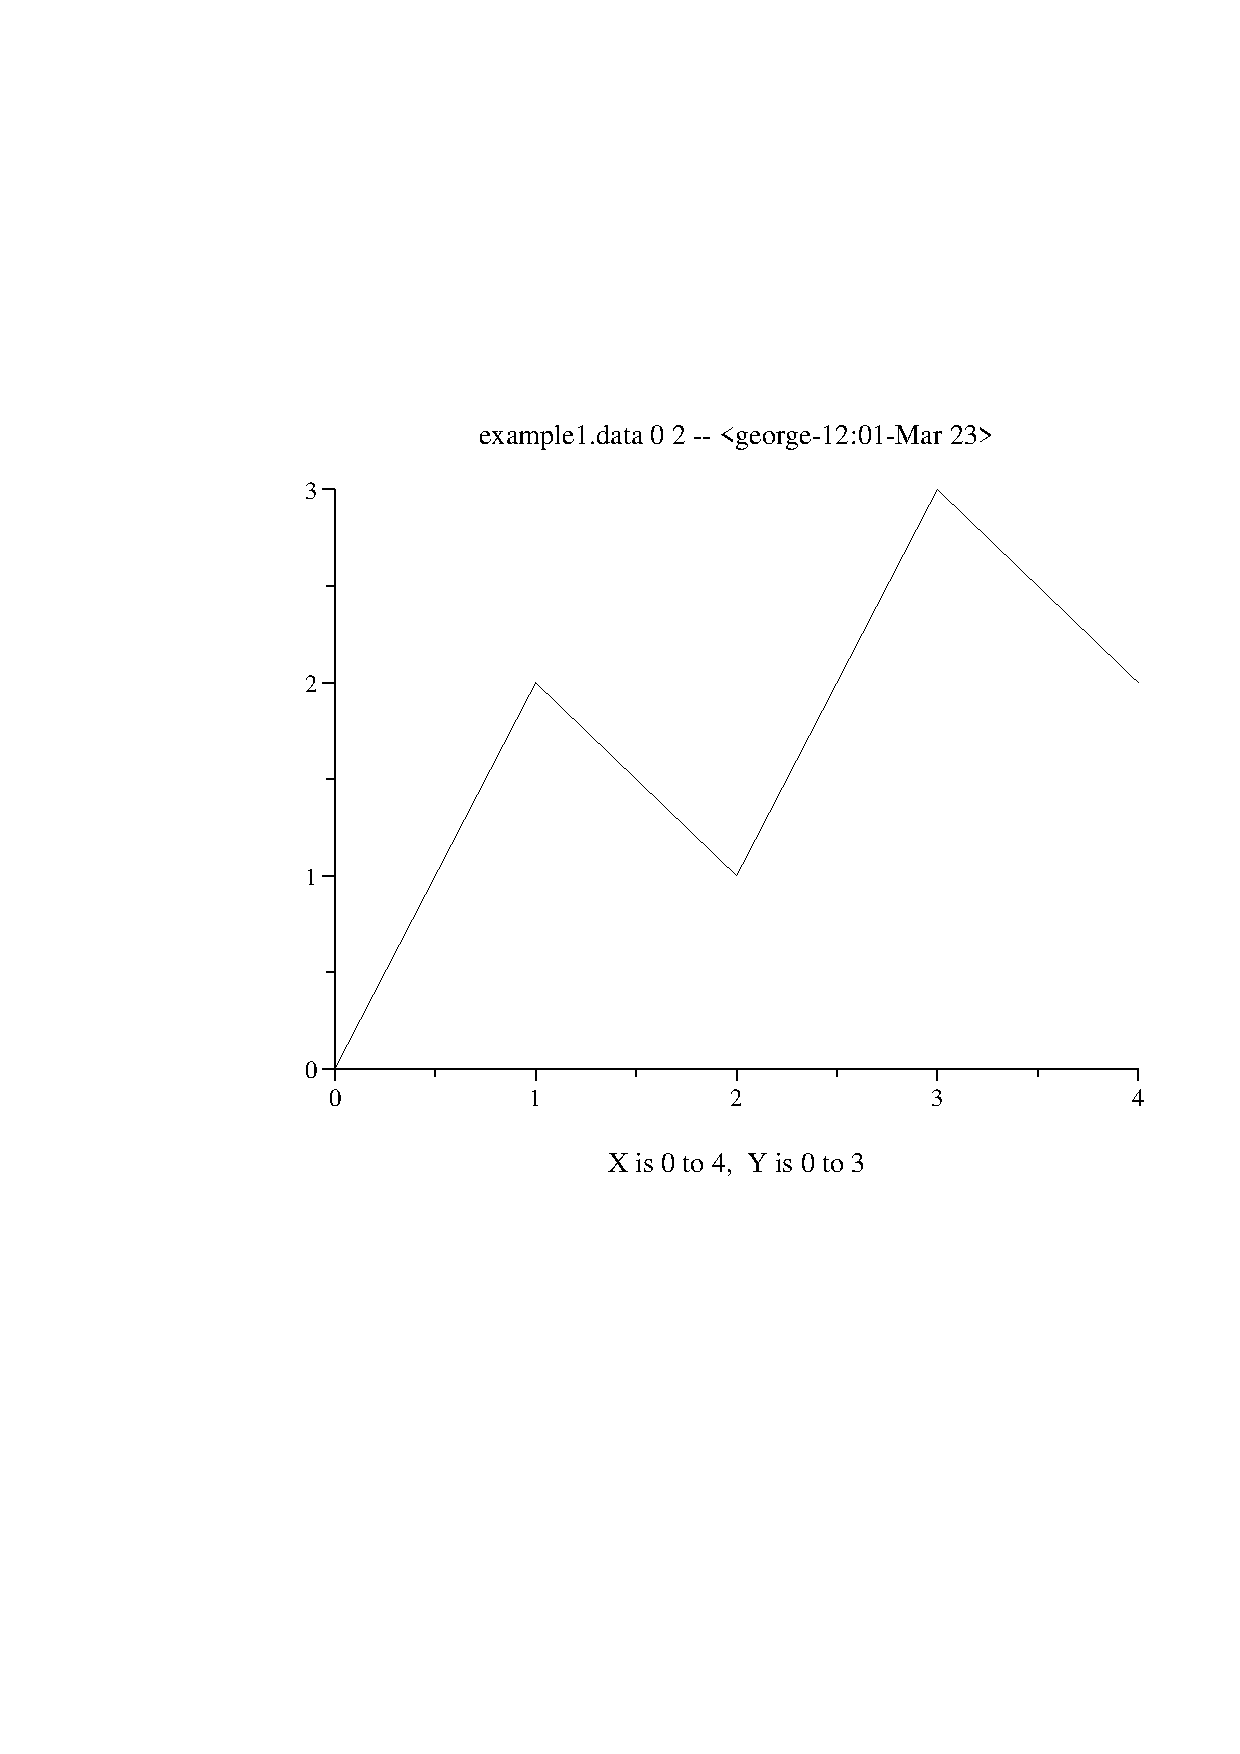
\epsfig{file=figure1,height=8cm}} &
{\vspace{-8cm}
{\em Data}
\vspace*{3mm}
\par
\begin{boxedverbatim}

0 0 0
1 1 2
2 3 1
3 5 3
4 7 2\end{boxedverbatim}

}
\end{tabular}
\end{center}

\begin{center}
\begin{boxedverbatim}

plt example1.data 0 2\end{boxedverbatim}

\end{center}
%
To see how to include {\tt plt} output as a figure in a \LaTeX {}
document such as this one, refer to appendix~\ref{sec:latex},
\emph{Including {\tt plt} figures in a \LaTeX {} document},
page~\pageref{sec:latex}.  The frame lines surrounding most of the
figures in this book show their bounding boxes (corresponding to
the borders of the {\tt plt} window for an on-screen plot, or of
the page for a printed plot.)
\end{figure}%
\lthtmlfigureZ
\lthtmlcheckvsize\clearpage}

\stepcounter{section}
\stepcounter{subsection}
{\newpage\clearpage
\lthtmlfigureA{figure465}%
\begin{figure}\begin{center}
\epsfig{file=simple0,height=8cm}

\end{center}
\end{figure}%
\lthtmlfigureZ
\lthtmlcheckvsize\clearpage}

{\newpage\clearpage
\lthtmlfigureA{figure471}%
\begin{figure}\begin{center}
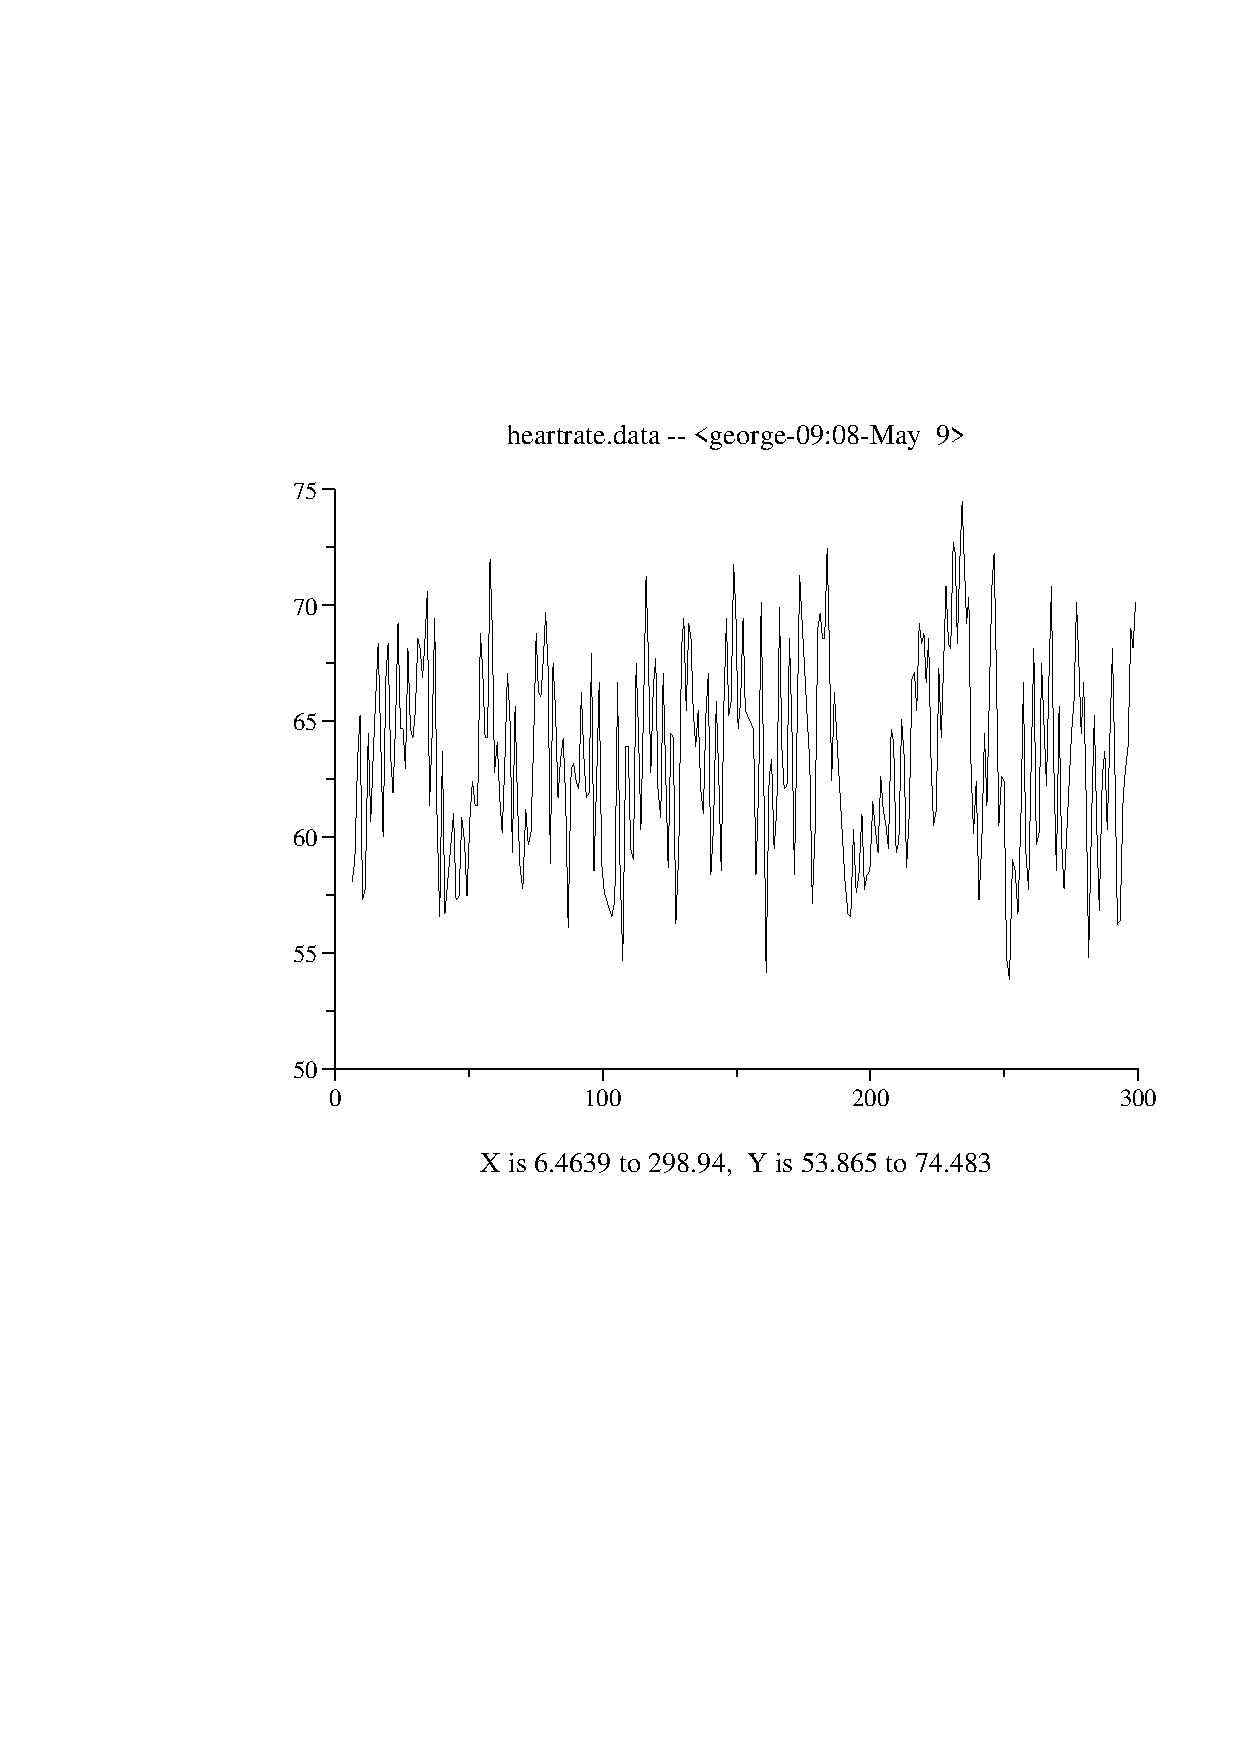
\epsfig{file=simple1,height=8cm}

\end{center}
\end{figure}%
\lthtmlfigureZ
\lthtmlcheckvsize\clearpage}

\stepcounter{subsection}
{\newpage\clearpage
\lthtmlinlinemathA{tex2html_wrap_inline3585}%
$\backslash$%
\lthtmlinlinemathZ
\lthtmlcheckvsize\clearpage}

{\newpage\clearpage
\lthtmlfigureA{figure494}%
\begin{figure}\begin{center}
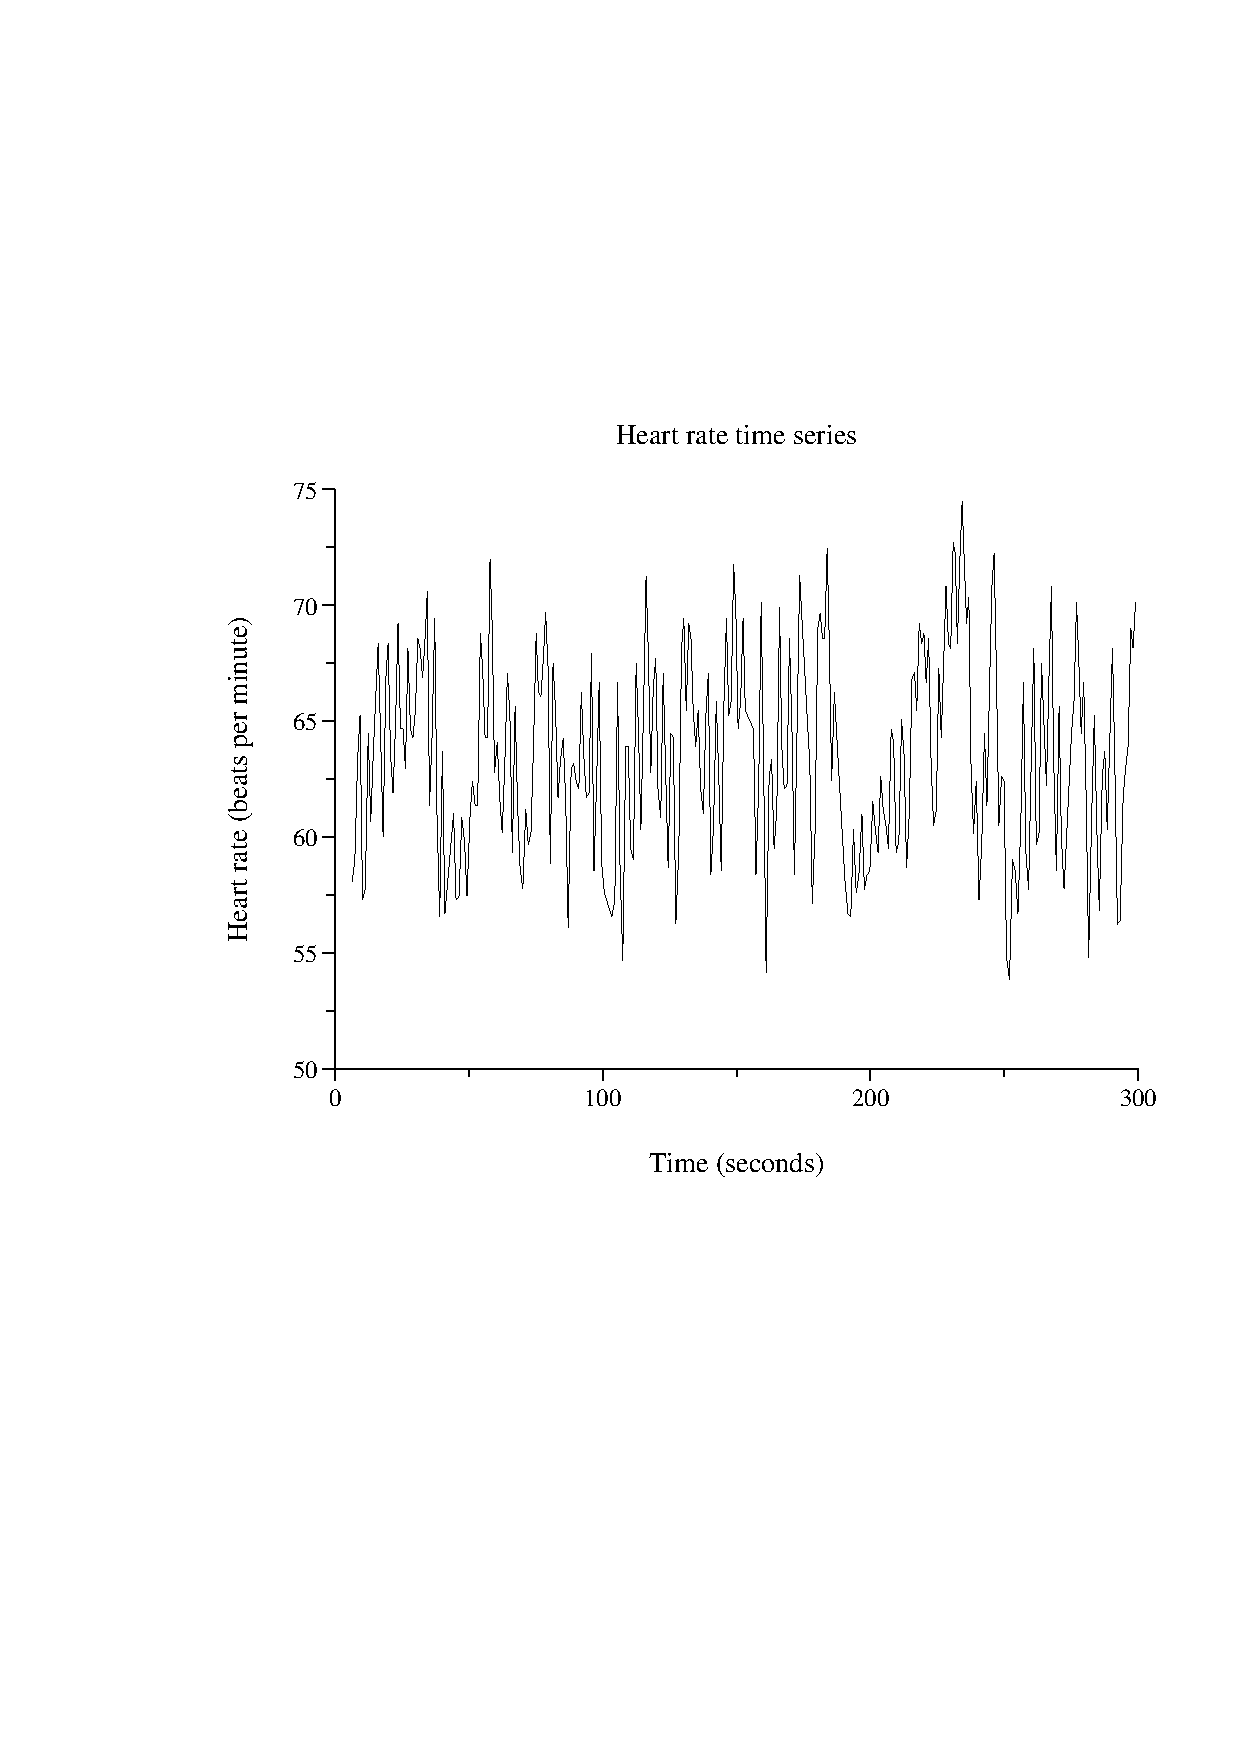
\epsfig{file=simple2,height=8cm}

\end{center}
\end{figure}%
\lthtmlfigureZ
\lthtmlcheckvsize\clearpage}

\stepcounter{subsection}
{\newpage\clearpage
\lthtmlfigureA{figure509}%
\begin{figure}\begin{center}
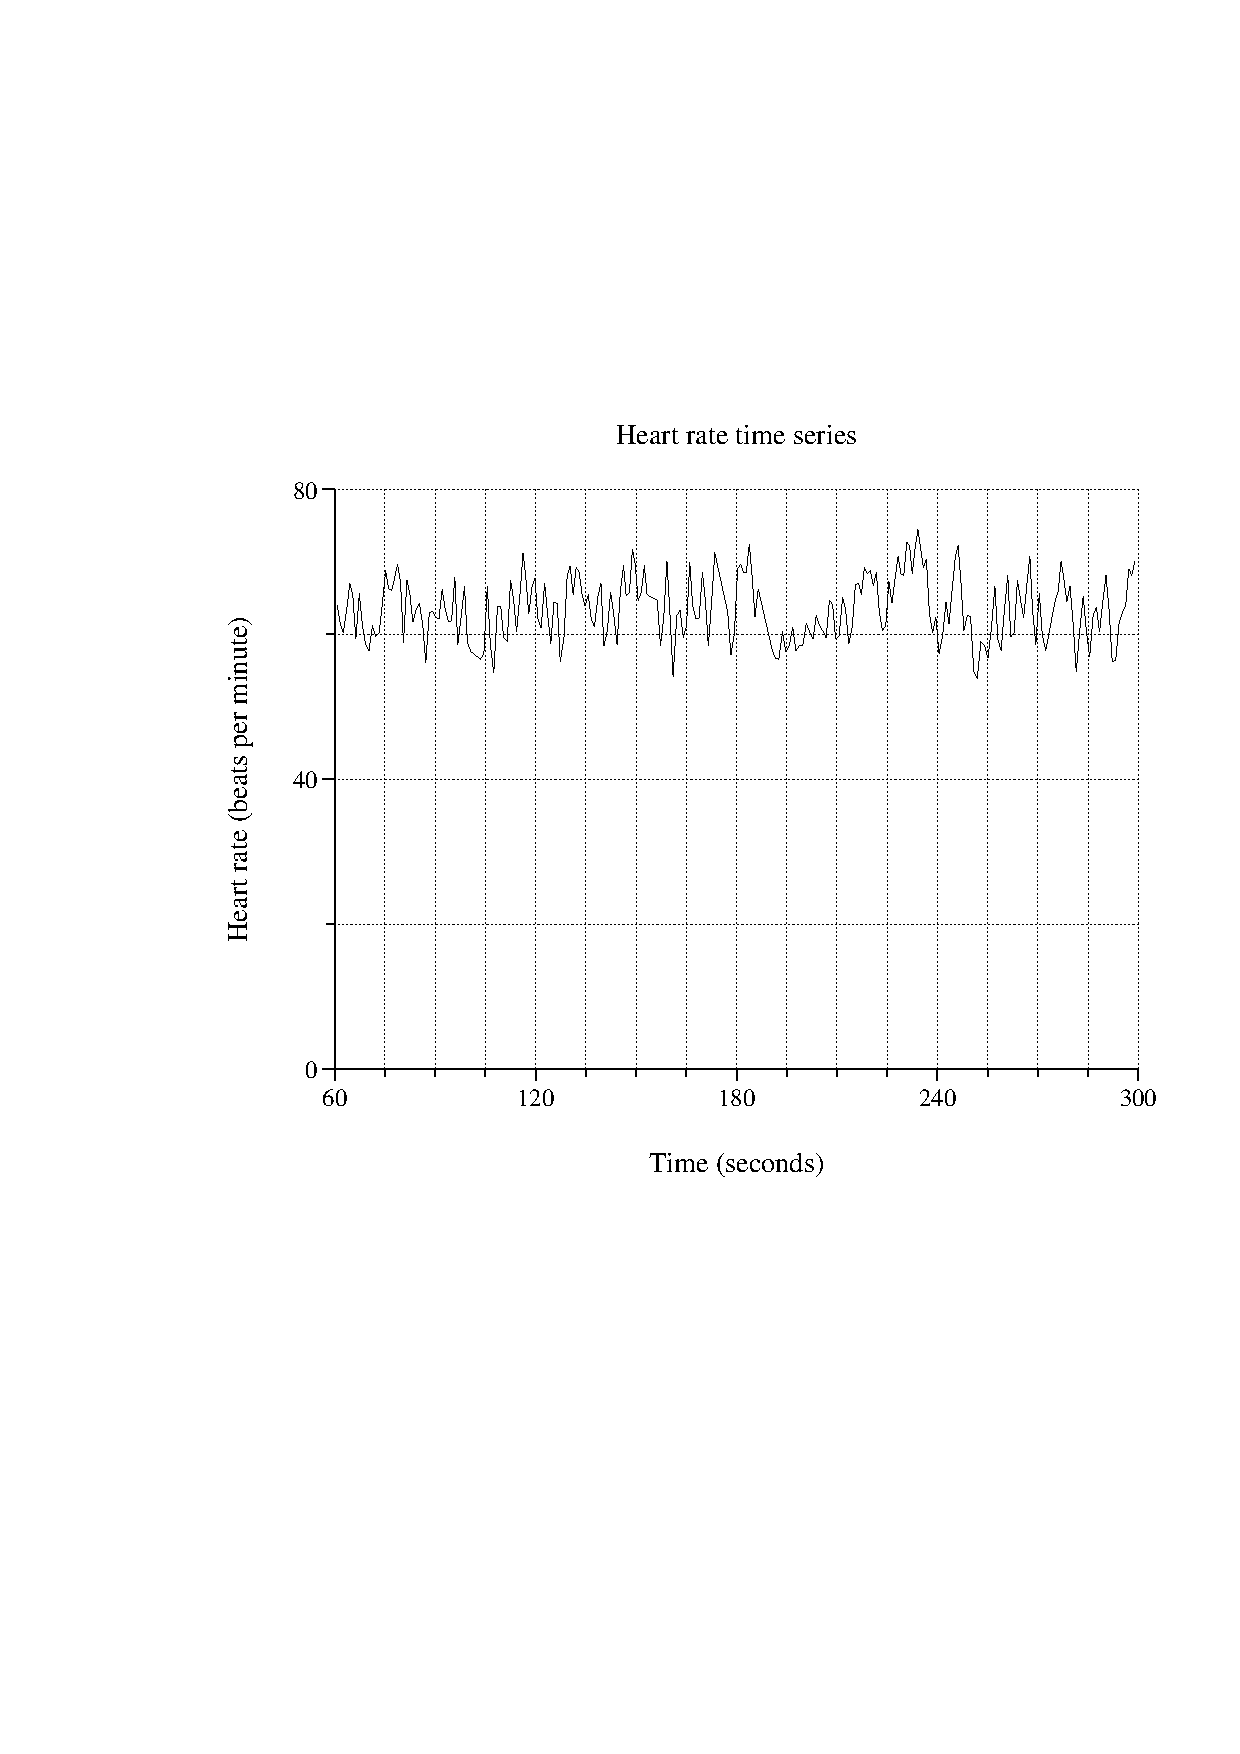
\epsfig{file=simple3,height=8cm}

\end{center}
\end{figure}%
\lthtmlfigureZ
\lthtmlcheckvsize\clearpage}

\stepcounter{subsection}
{\newpage\clearpage
\lthtmlfigureA{figure559}%
\begin{figure}\begin{center}
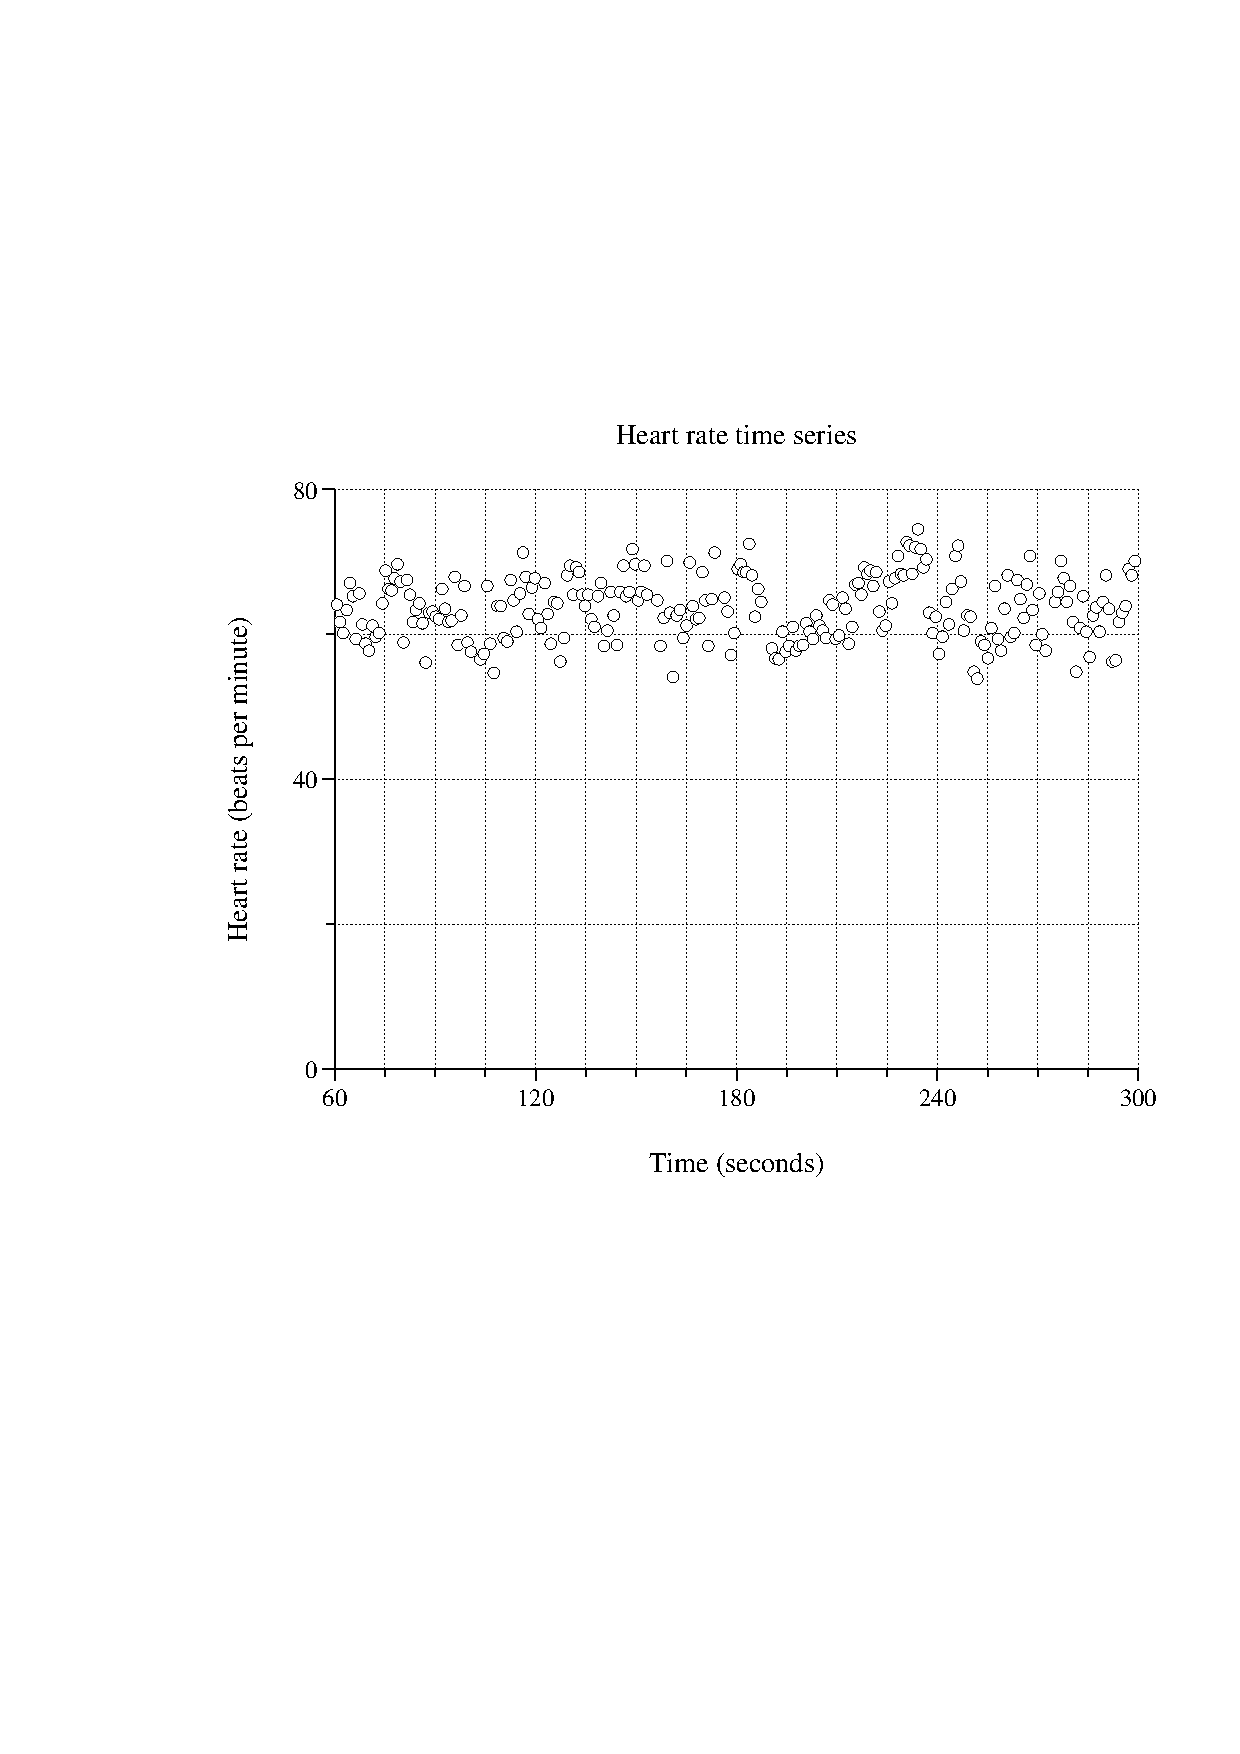
\epsfig{file=simple4,height=8cm}

\end{center}
\end{figure}%
\lthtmlfigureZ
\lthtmlcheckvsize\clearpage}

\stepcounter{subsection}
{\newpage\clearpage
\lthtmlfigureA{figure579}%
\begin{figure}\begin{center}
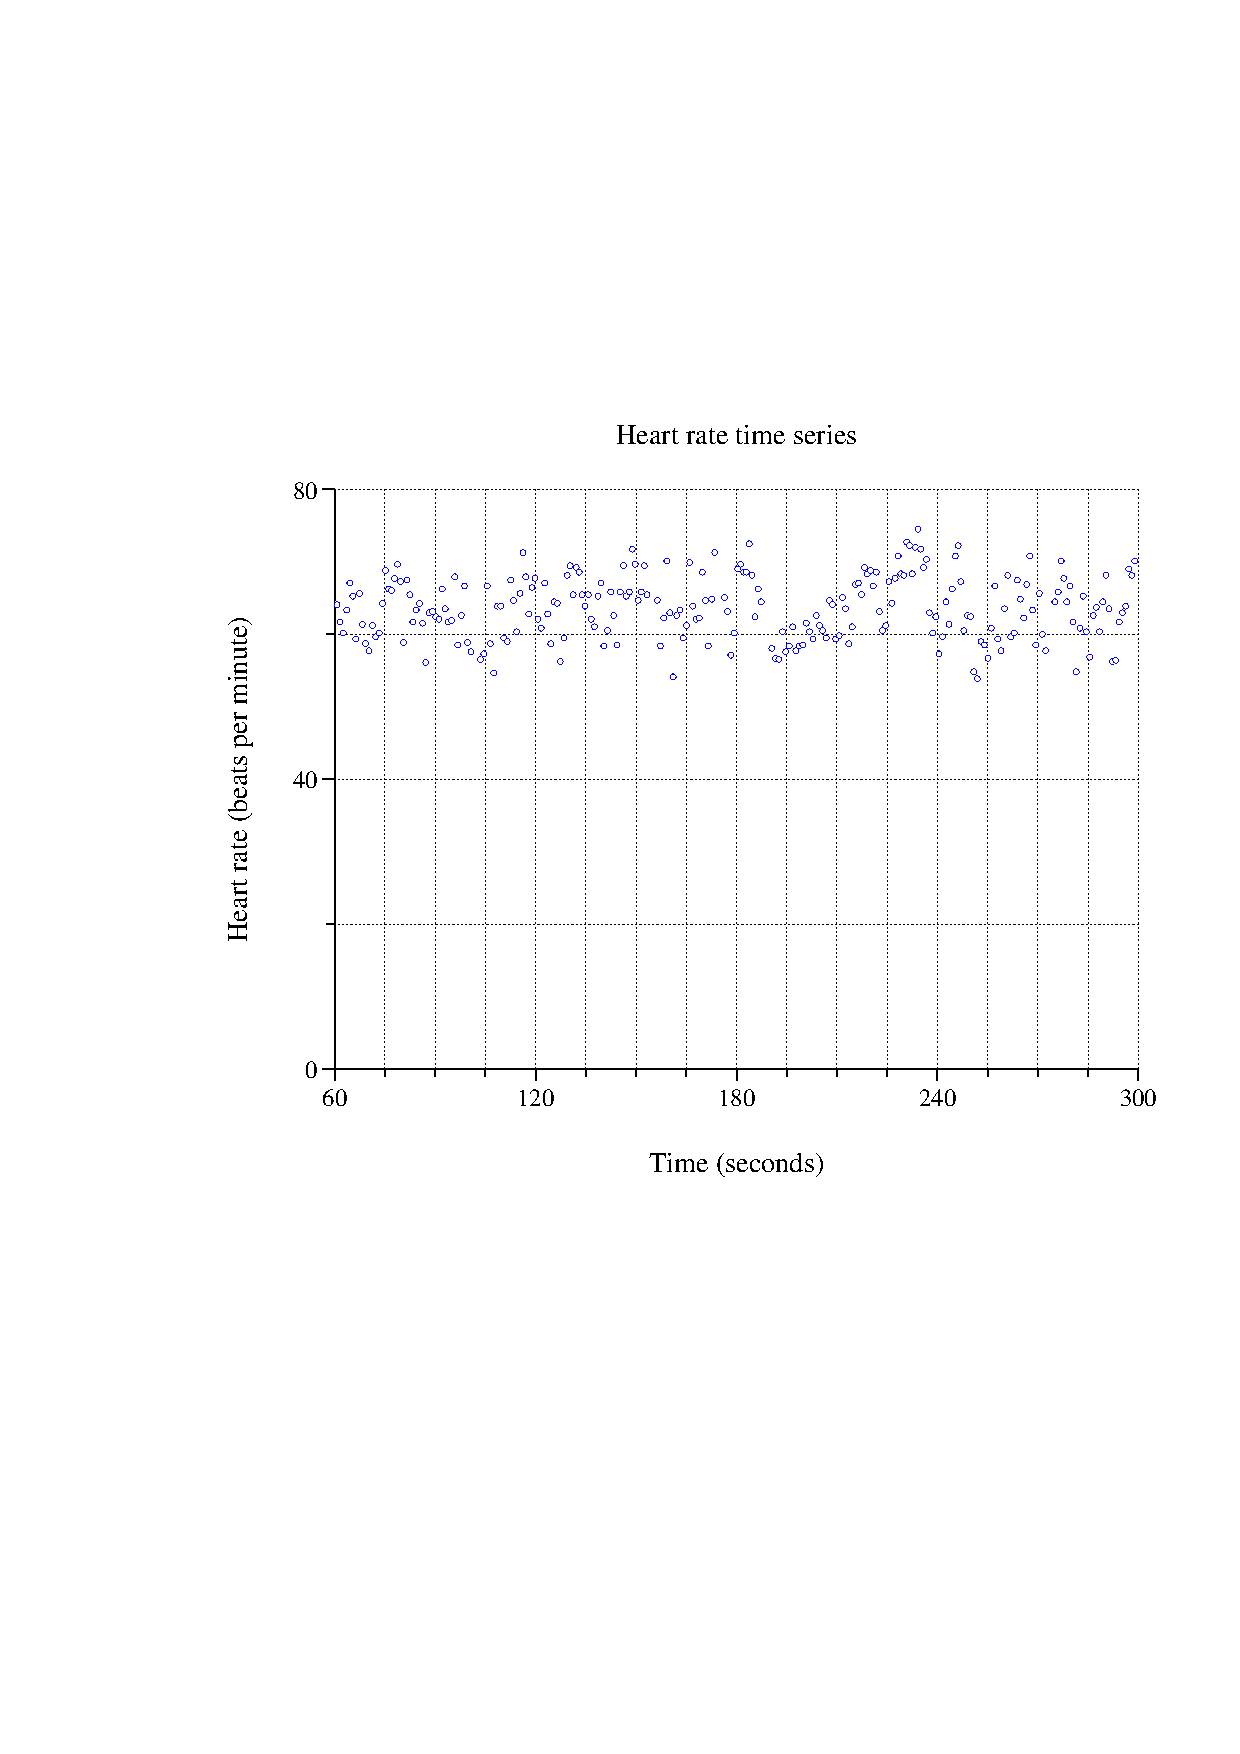
\epsfig{file=simple5,height=8cm}

\end{center}
\end{figure}%
\lthtmlfigureZ
\lthtmlcheckvsize\clearpage}

\stepcounter{section}
{\newpage\clearpage
\lthtmlfigureA{figure605}%
\begin{figure}\begin{center}
\fcolorbox{blue}{white}{
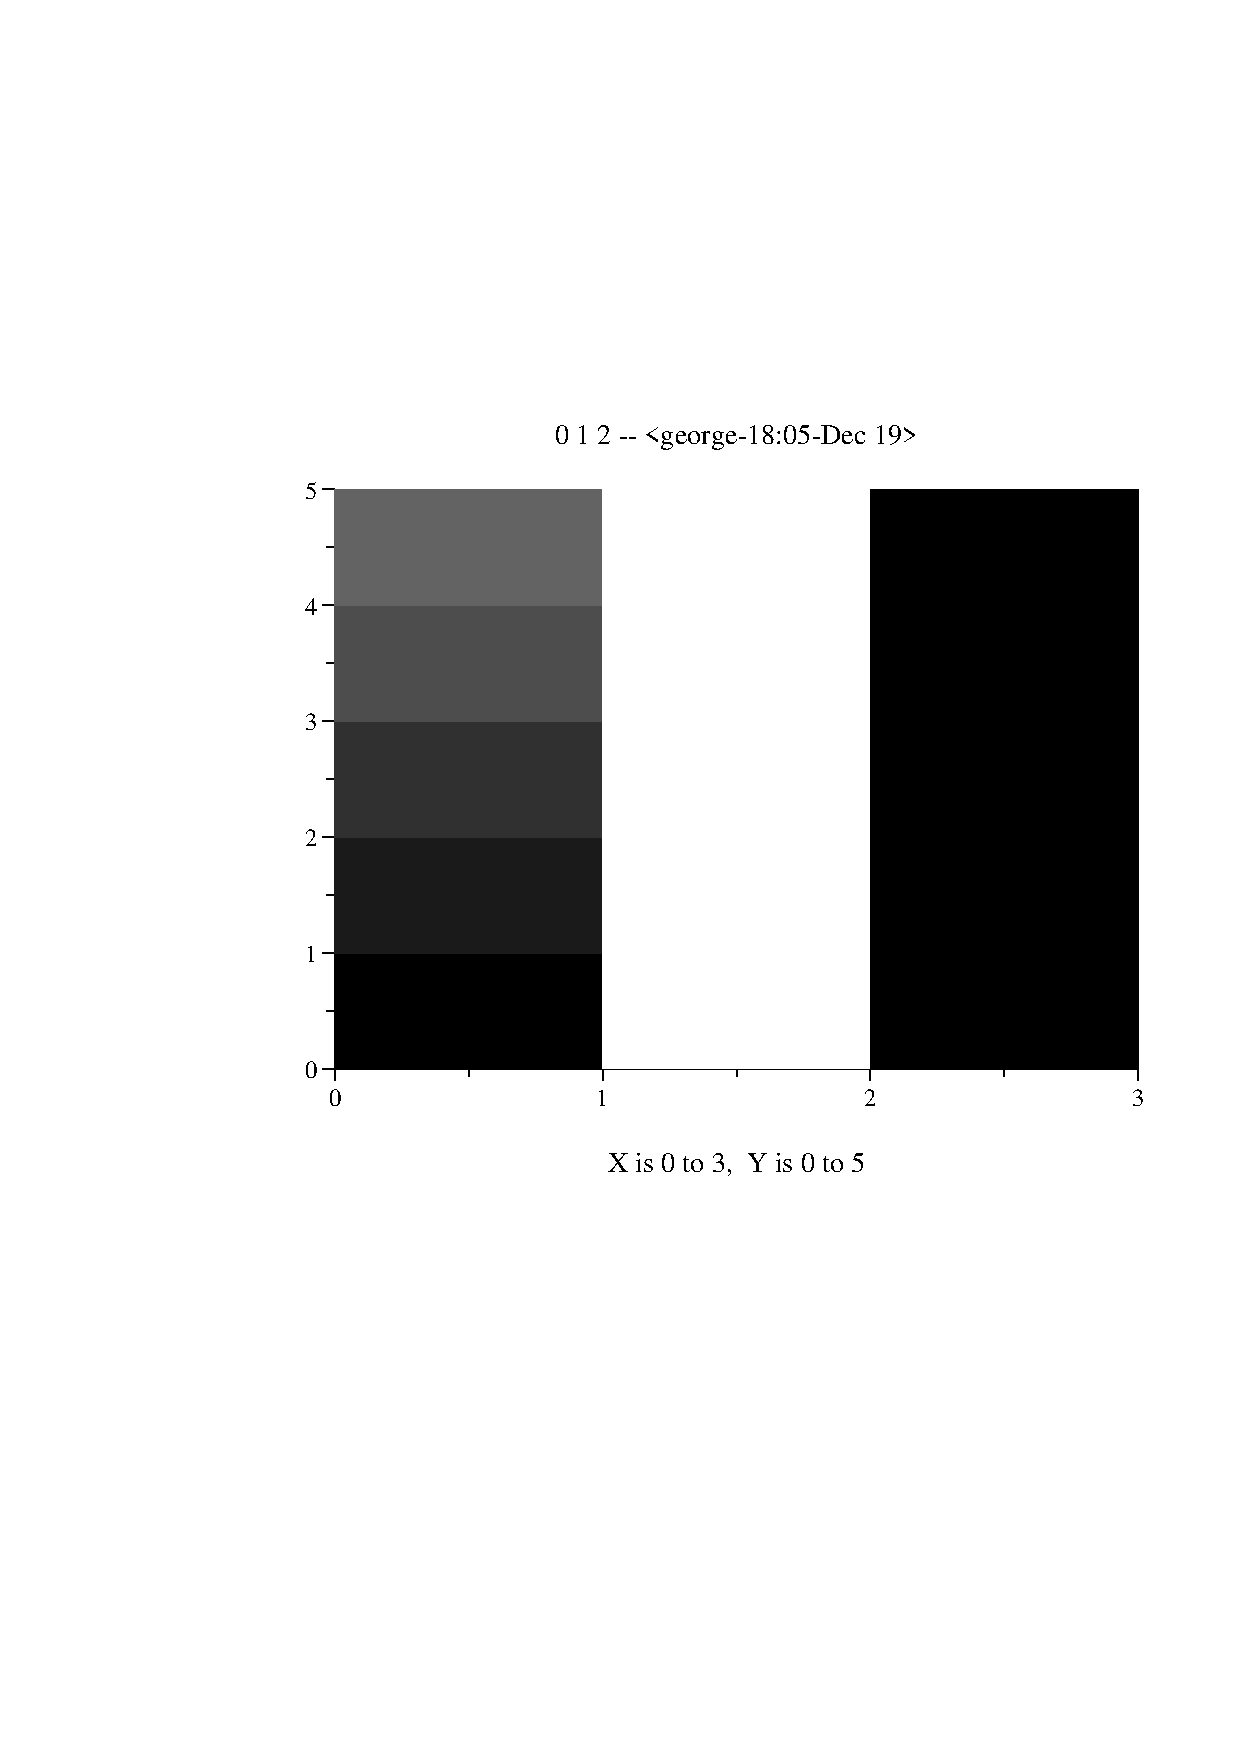
\epsfig{file=image,height=10cm}}
\end{center}

\begin{center}
\begin{boxedverbatim}

imageplt -d 5 3 image.data | plt 0 1 2 -pc\end{boxedverbatim}

\end{center}
\end{figure}%
\lthtmlfigureZ
\lthtmlcheckvsize\clearpage}

\stepcounter{section}
{\newpage\clearpage
\lthtmlinlinemathA{tex2html_wrap_inline3587}%
$f(x)=x^2-4x+7$%
\lthtmlinlinemathZ
\lthtmlcheckvsize\clearpage}

{\newpage\clearpage
\lthtmlinlinemathA{tex2html_wrap_inline3589}%
$x$%
\lthtmlinlinemathZ
\lthtmlcheckvsize\clearpage}

{\newpage\clearpage
\lthtmlfigureA{figure667}%
\begin{figure}\begin{center}
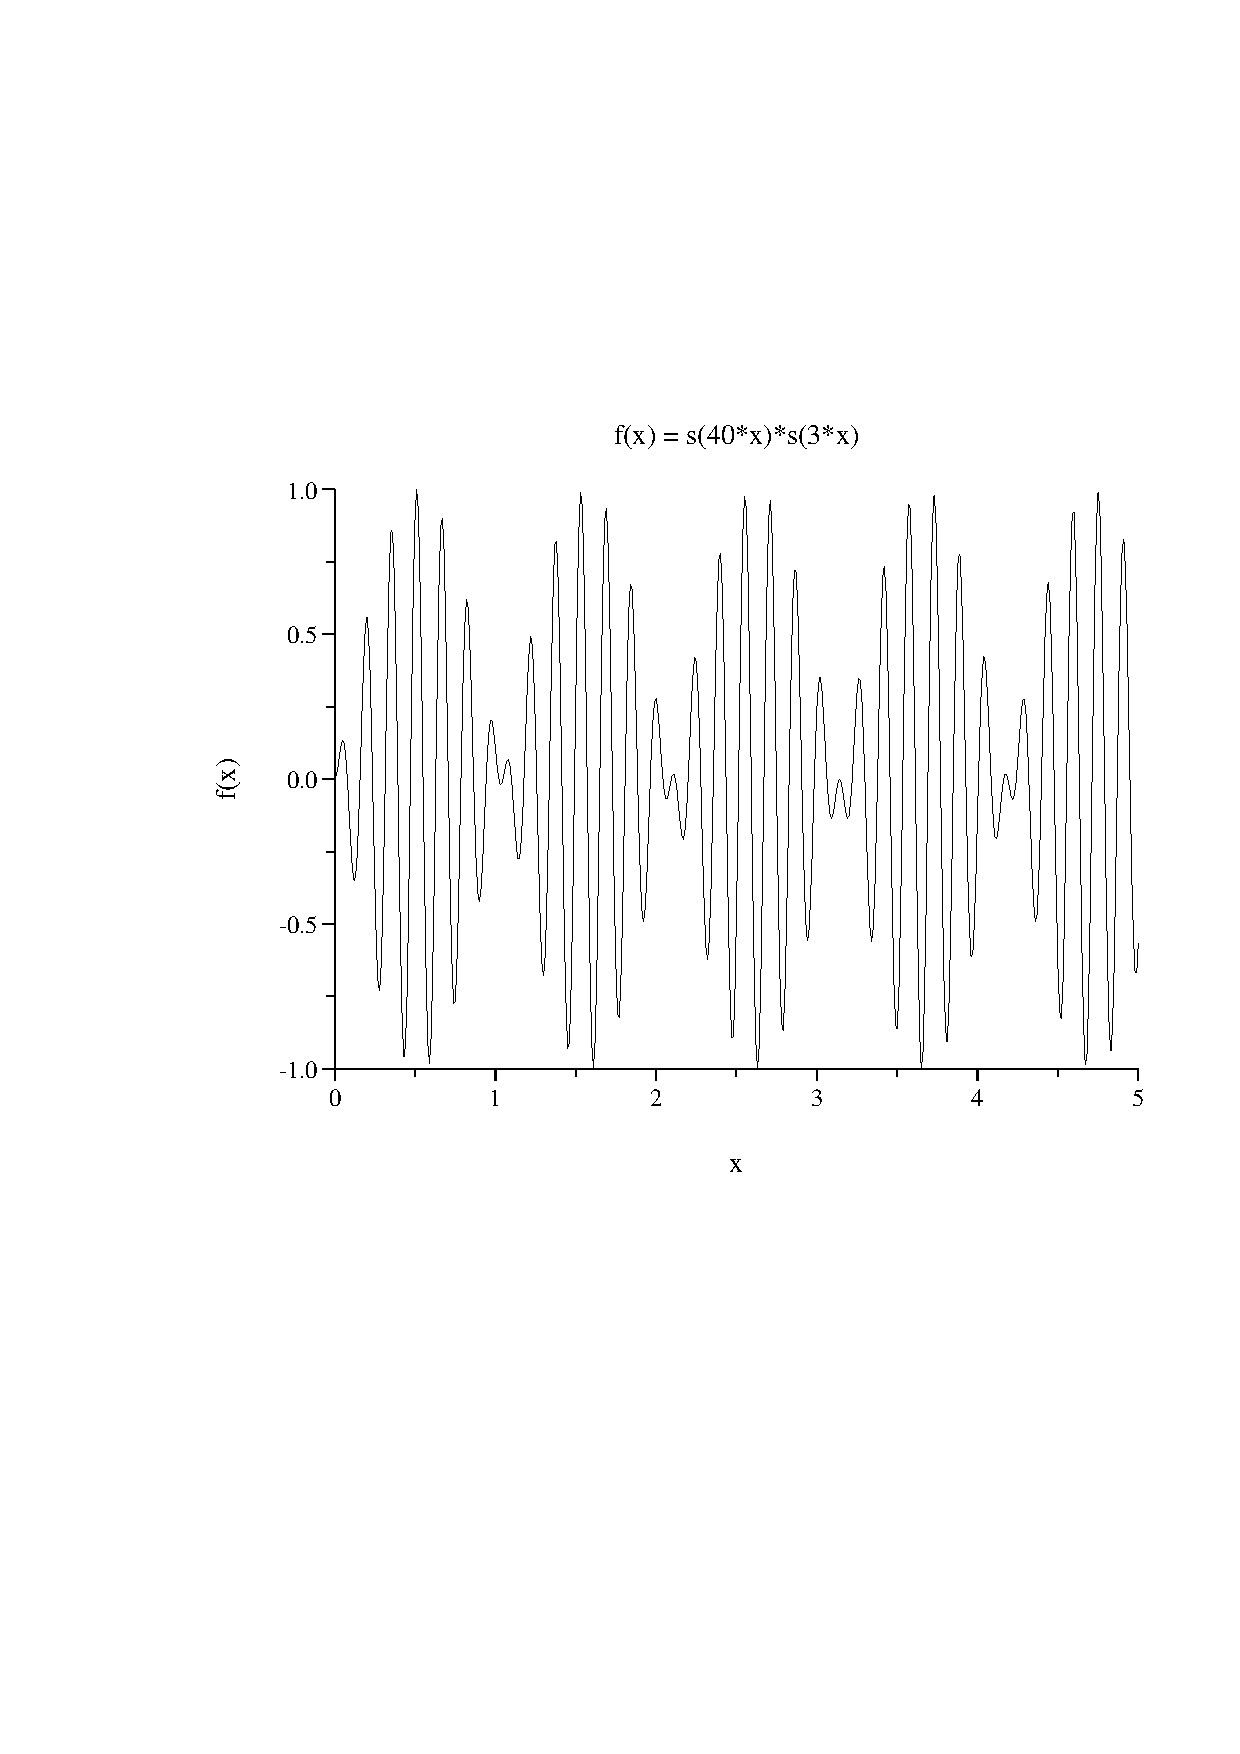
\epsfig{file=function,height=8cm}

\end{center}
\end{figure}%
\lthtmlfigureZ
\lthtmlcheckvsize\clearpage}

\stepcounter{chapter}
\stepcounter{section}
\stepcounter{section}
\stepcounter{section}
{\newpage\clearpage
\lthtmlinlinemathA{tex2html_wrap_inline3593}%
$N$%
\lthtmlinlinemathZ
\lthtmlcheckvsize\clearpage}

\stepcounter{section}
{\newpage\clearpage
\lthtmlinlinemathA{tex2html_wrap_inline5179}%
\fbox{{\tt dd ibs=1 skip=}{\em nbytes} {\tt <}{\em data-file} {\tt | plt ...}}%
\lthtmlinlinemathZ
\lthtmlcheckvsize\clearpage}

\stepcounter{section}
{\newpage\clearpage
\lthtmlinlinemathA{tex2html_wrap_inline3597}%
$x_{from}$%
\lthtmlinlinemathZ
\lthtmlcheckvsize\clearpage}

{\newpage\clearpage
\lthtmlinlinemathA{tex2html_wrap_inline3599}%
$x_{incr}$%
\lthtmlinlinemathZ
\lthtmlcheckvsize\clearpage}

{\newpage\clearpage
\lthtmlinlinemathA{tex2html_wrap_inline3601}%
$x_{from} \ \ x_{incr}$%
\lthtmlinlinemathZ
\lthtmlcheckvsize\clearpage}

{\newpage\clearpage
\lthtmlinlinemathA{tex2html_wrap_inline3605}%
$\frac{1}{128}$%
\lthtmlinlinemathZ
\lthtmlcheckvsize\clearpage}

{\newpage\clearpage
\lthtmlinlinemathA{tex2html_wrap_inline3607}%
$8 \cdot 128$%
\lthtmlinlinemathZ
\lthtmlcheckvsize\clearpage}

{\newpage\clearpage
\lthtmlfigureA{figure794}%
\begin{figure}\begin{center}
\fcolorbox{blue}{white}{
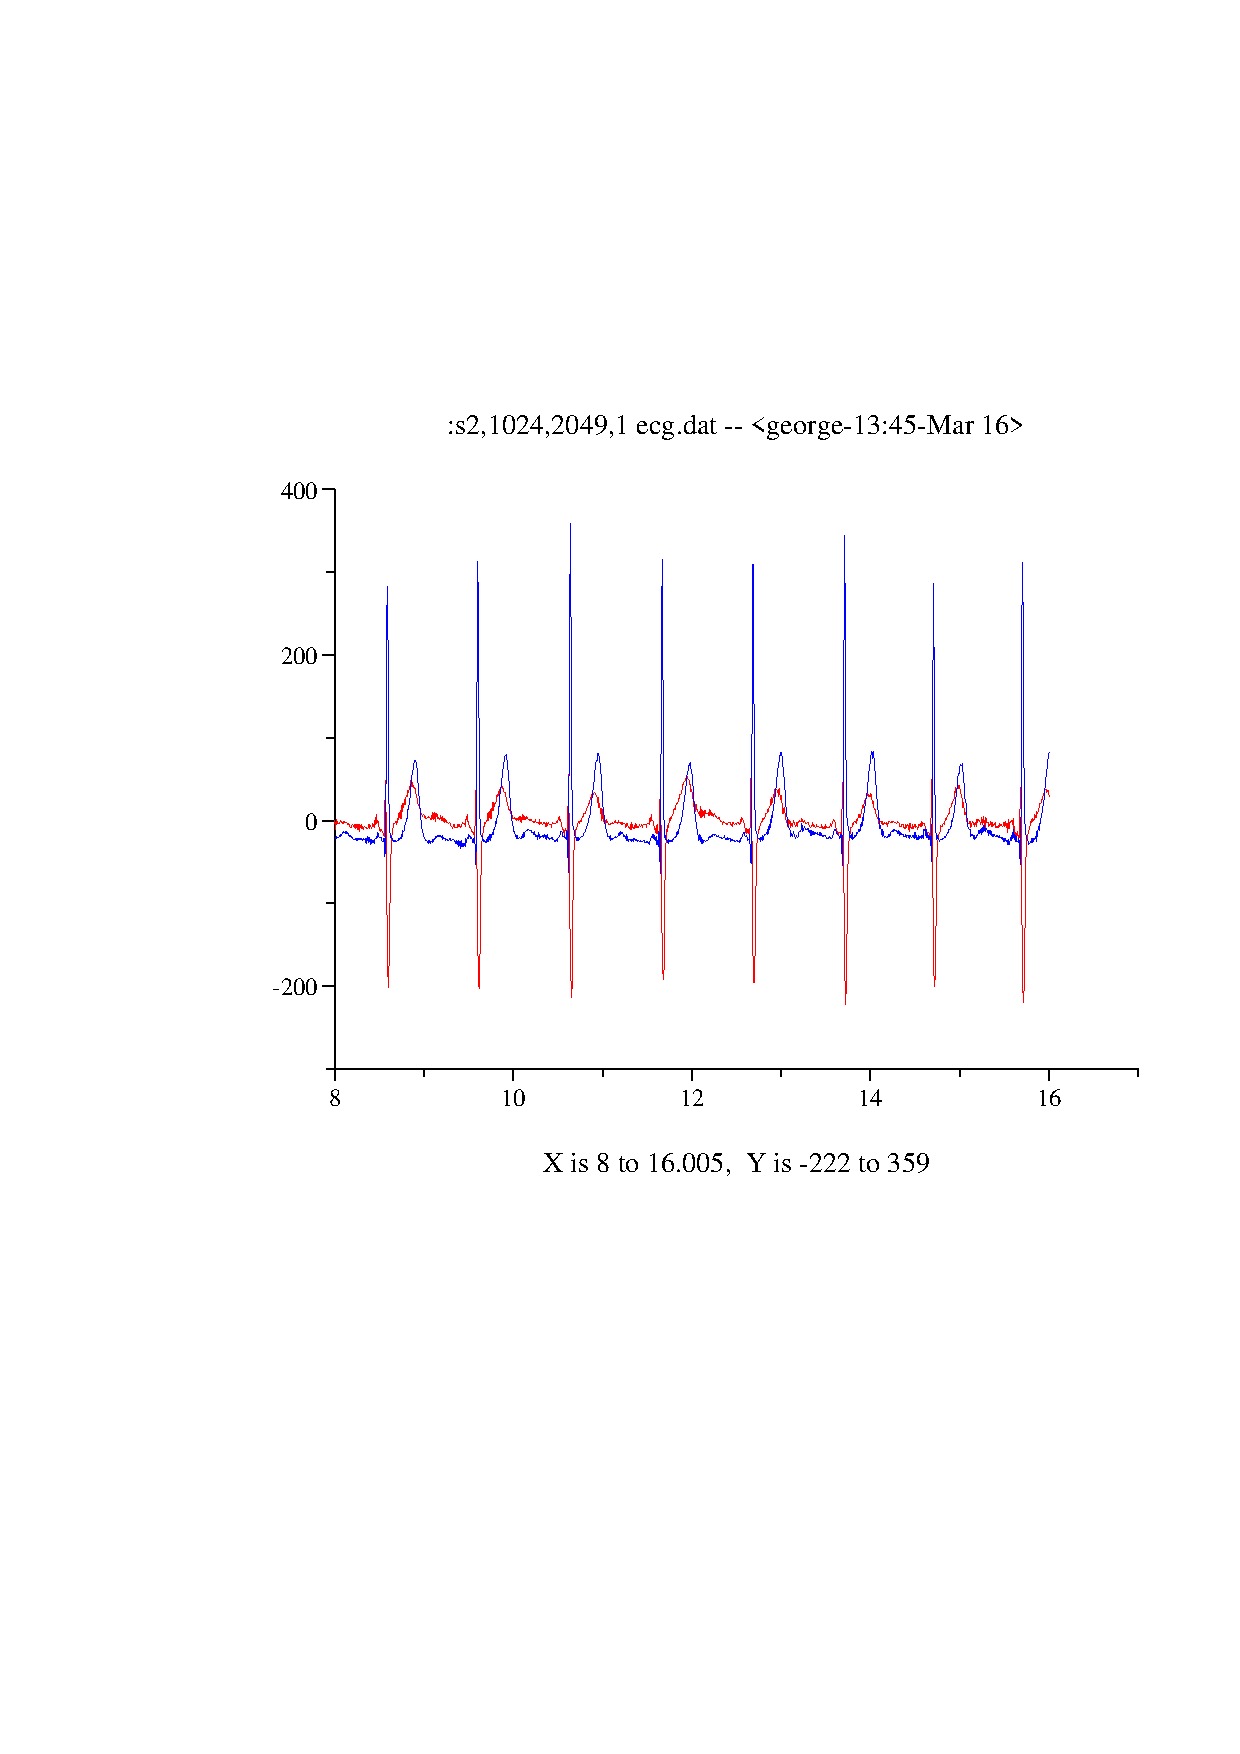
\epsfig{file=ecg,height=10cm}}

\begin{center}
\begin{boxedverbatim}

plt :s2,1024,2049,1 ecg.dat \
    -cz 8 .00781 -F"p 0,1n(Cred) 0,2n(Cblue)"\end{boxedverbatim}

\end{center}
\end{center}
\end{figure}%
\lthtmlfigureZ
\lthtmlcheckvsize\clearpage}

\stepcounter{section}
\stepcounter{section}
{\newpage\clearpage
\lthtmlinlinemathA{tex2html_wrap_inline3611}%
$string_{0} \ \  string_{1} \ \  ...$%
\lthtmlinlinemathZ
\lthtmlcheckvsize\clearpage}

\stepcounter{chapter}
{\newpage\clearpage
\lthtmlinlinemathA{tex2html_wrap_inline3617}%
$y$%
\lthtmlinlinemathZ
\lthtmlcheckvsize\clearpage}

{\newpage\clearpage
\lthtmlinlinemathA{tex2html_wrap_inline3619}%
$(x_{min},y_{min})$%
\lthtmlinlinemathZ
\lthtmlcheckvsize\clearpage}

{\newpage\clearpage
\lthtmlinlinemathA{tex2html_wrap_inline3621}%
$(x_{max},y_{max})$%
\lthtmlinlinemathZ
\lthtmlcheckvsize\clearpage}

{\newpage\clearpage
\lthtmlinlinemathA{tex2html_wrap_inline3623}%
$(xw,yw)$%
\lthtmlinlinemathZ
\lthtmlcheckvsize\clearpage}

{\newpage\clearpage
\lthtmlinlinemathA{tex2html_wrap_inline3625}%
$(0,0)$%
\lthtmlinlinemathZ
\lthtmlcheckvsize\clearpage}

{\newpage\clearpage
\lthtmlinlinemathA{tex2html_wrap_inline3627}%
$(1,1)$%
\lthtmlinlinemathZ
\lthtmlcheckvsize\clearpage}

{\newpage\clearpage
\lthtmlinlinemathA{tex2html_wrap_inline3637}%
$(xp,yp)$%
\lthtmlinlinemathZ
\lthtmlcheckvsize\clearpage}

{\newpage\clearpage
\lthtmlfigureA{figure896}%
\begin{figure}\begin{center}
\fcolorbox{blue}{white}{
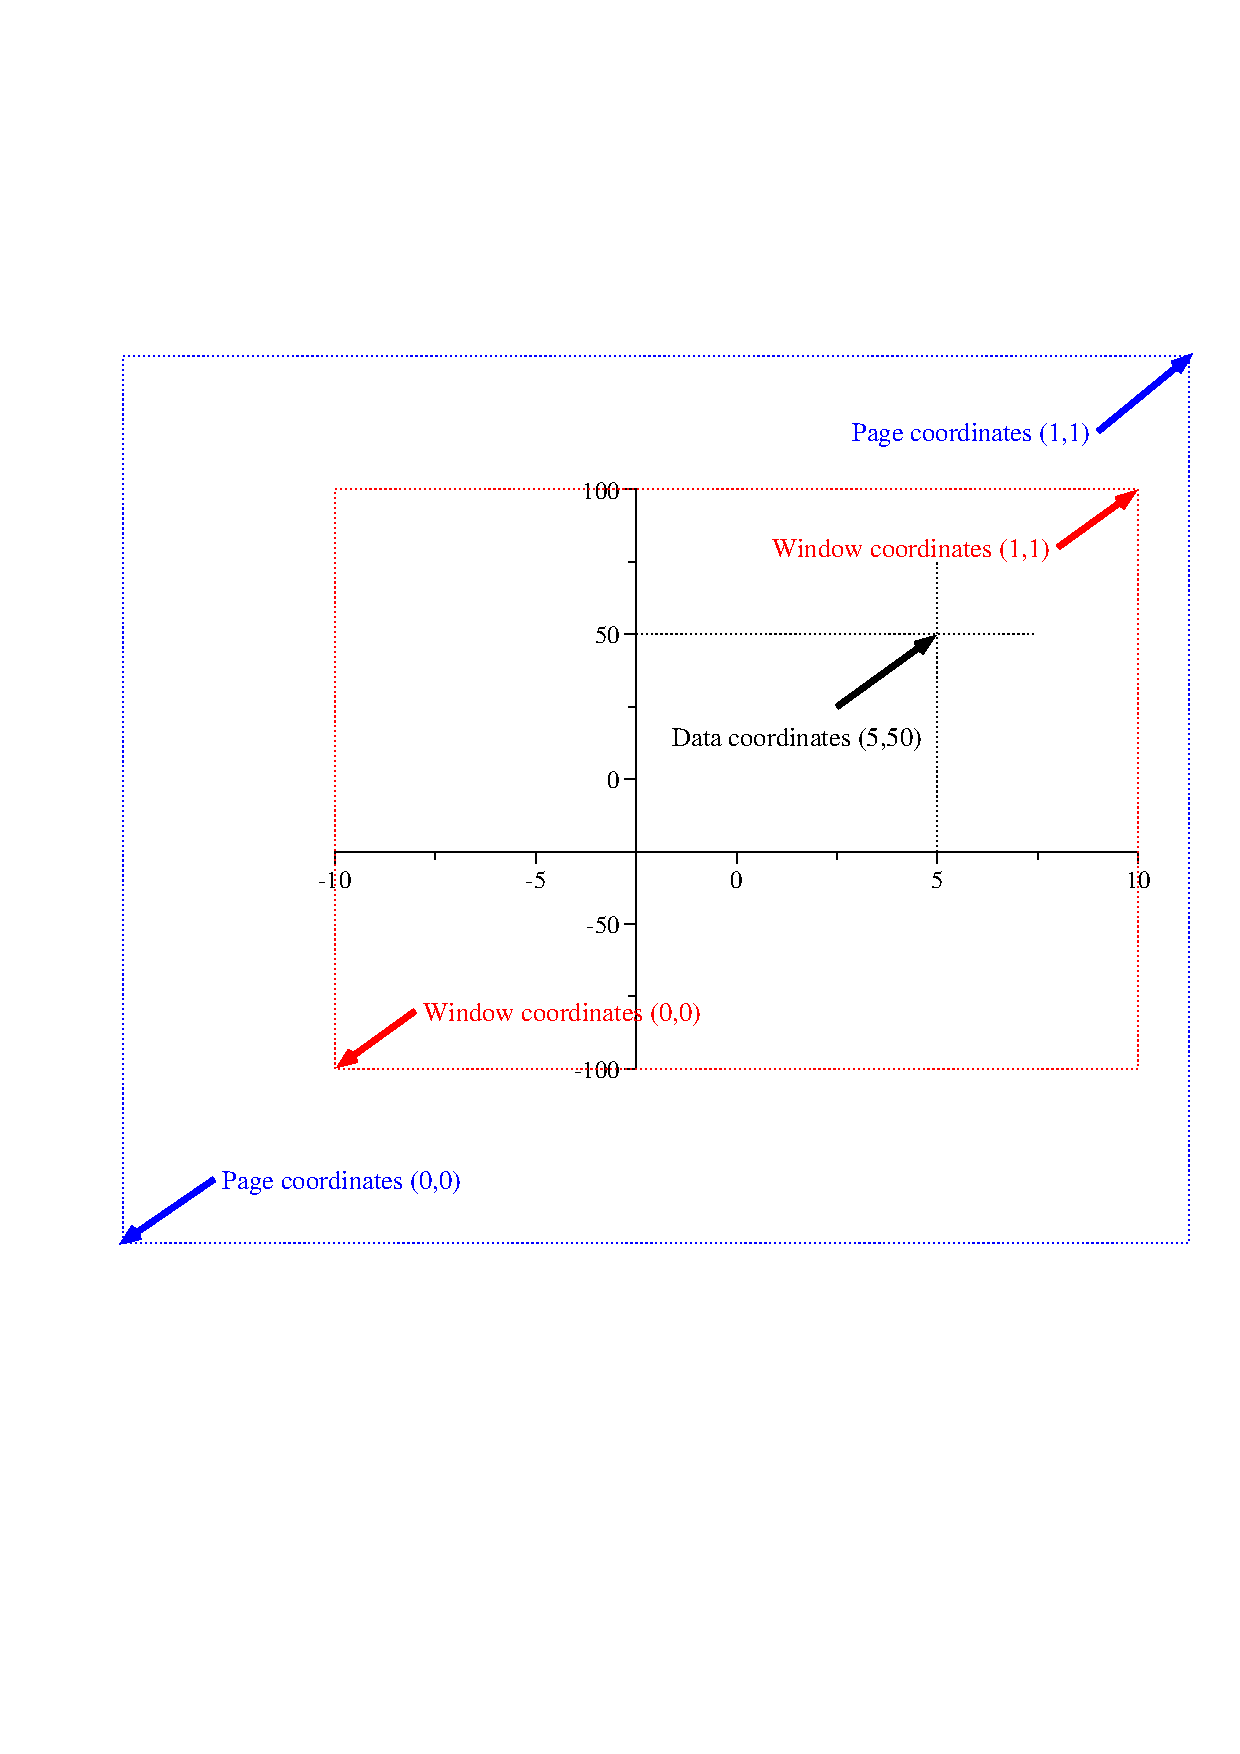
\epsfig{file=coords,height=10cm}}
\end{center}

\end{figure}%
\lthtmlfigureZ
\lthtmlcheckvsize\clearpage}

{\newpage\clearpage
\lthtmlinlinemathA{tex2html_wrap_inline3643}%
$(x,y)$%
\lthtmlinlinemathZ
\lthtmlcheckvsize\clearpage}

{\newpage\clearpage
\lthtmlfigureA{figure919}%
\begin{figure}\begin{center}
\fcolorbox{blue}{white}{
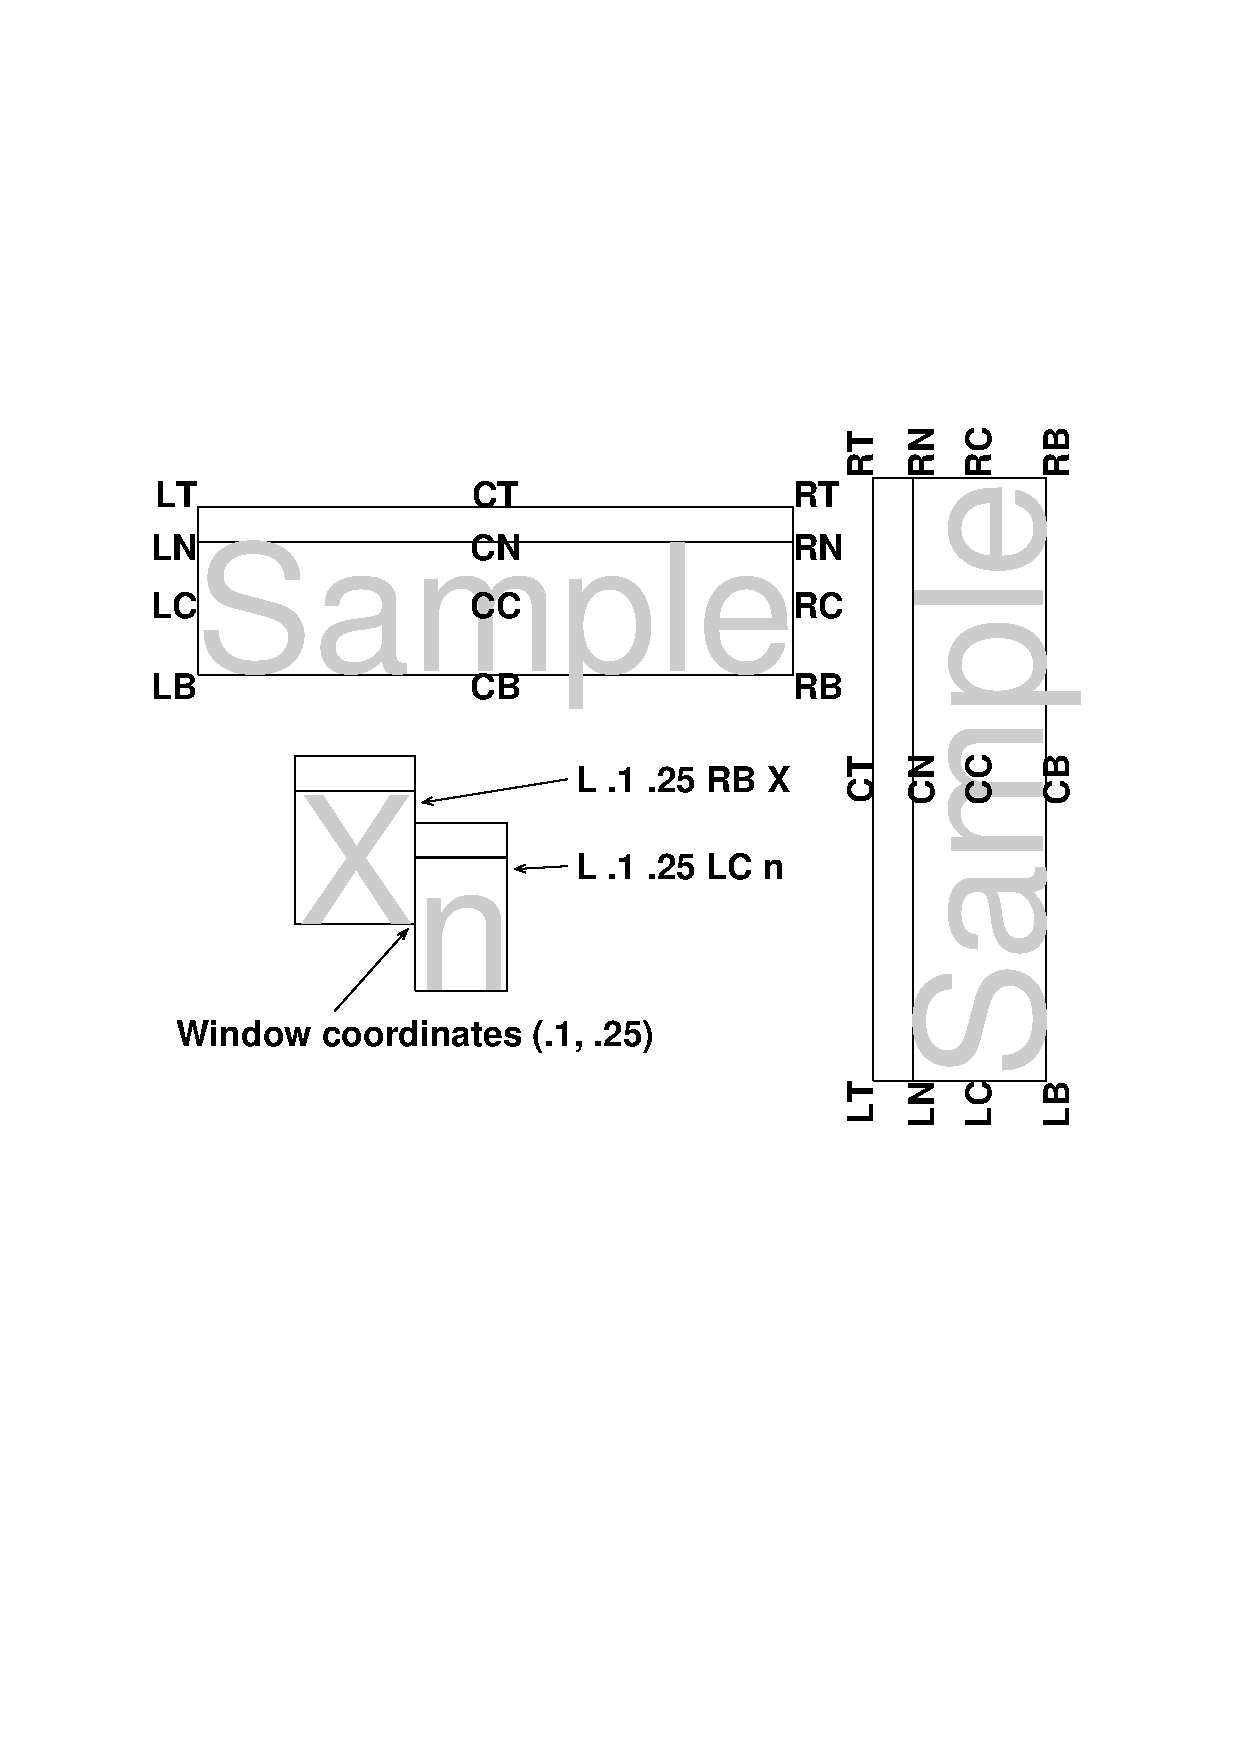
\epsfig{file=figure8,height=10cm}}
\end{center}
%

\end{figure}%
\lthtmlfigureZ
\lthtmlcheckvsize\clearpage}

\stepcounter{chapter}
{\newpage\clearpage
\lthtmlfigureA{figure949}%
\begin{figure}\begin{center}
\fcolorbox{blue}{white}{
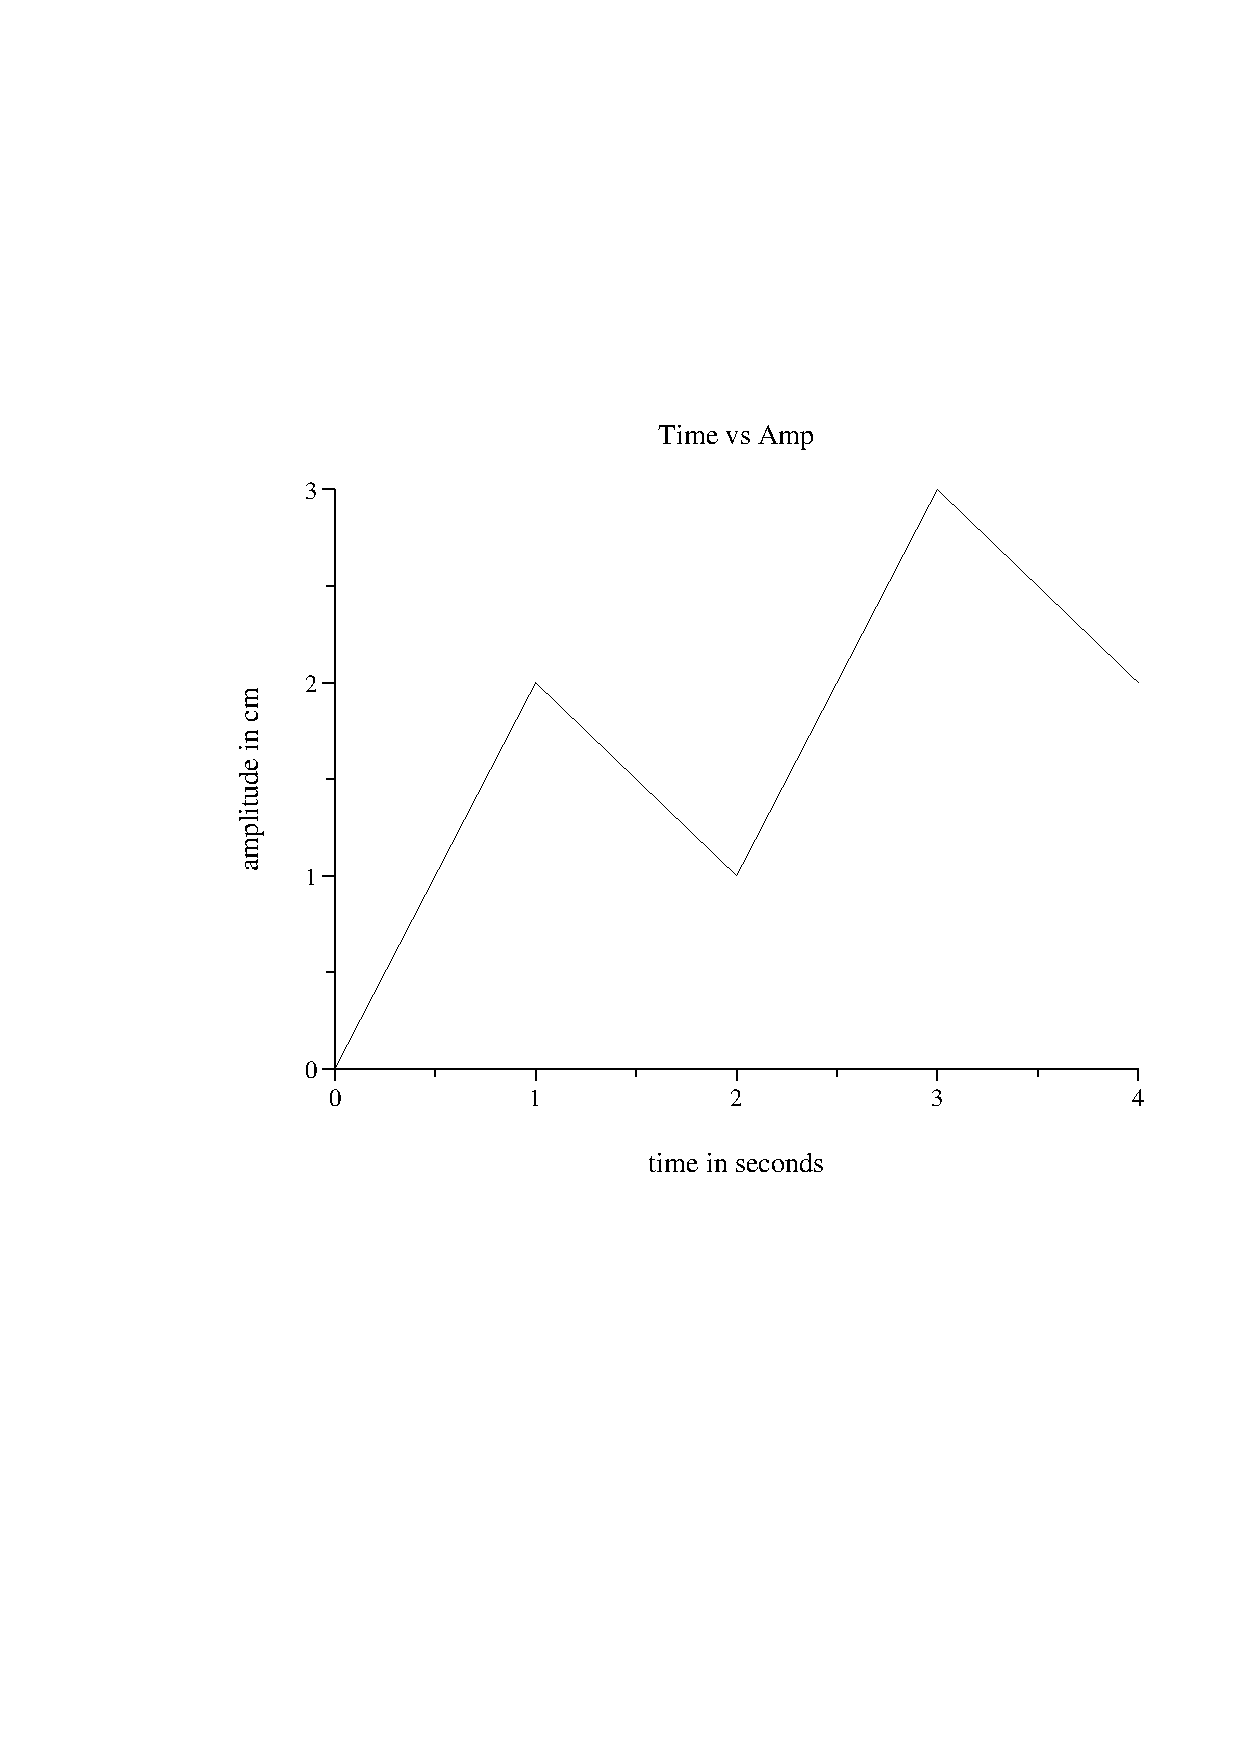
\epsfig{file=figure2,height=10cm}}
\end{center}

\begin{center}
\begin{boxedverbatim}

plt example1.data 0 2  -t "Time vs Amp" \
    -x "time in seconds" -y "amplitude in cm"\end{boxedverbatim}

\end{center}
\end{figure}%
\lthtmlfigureZ
\lthtmlcheckvsize\clearpage}

{\newpage\clearpage
\lthtmlfigureA{figure1008}%
\begin{figure}\begin{center}
\fcolorbox{blue}{white}{
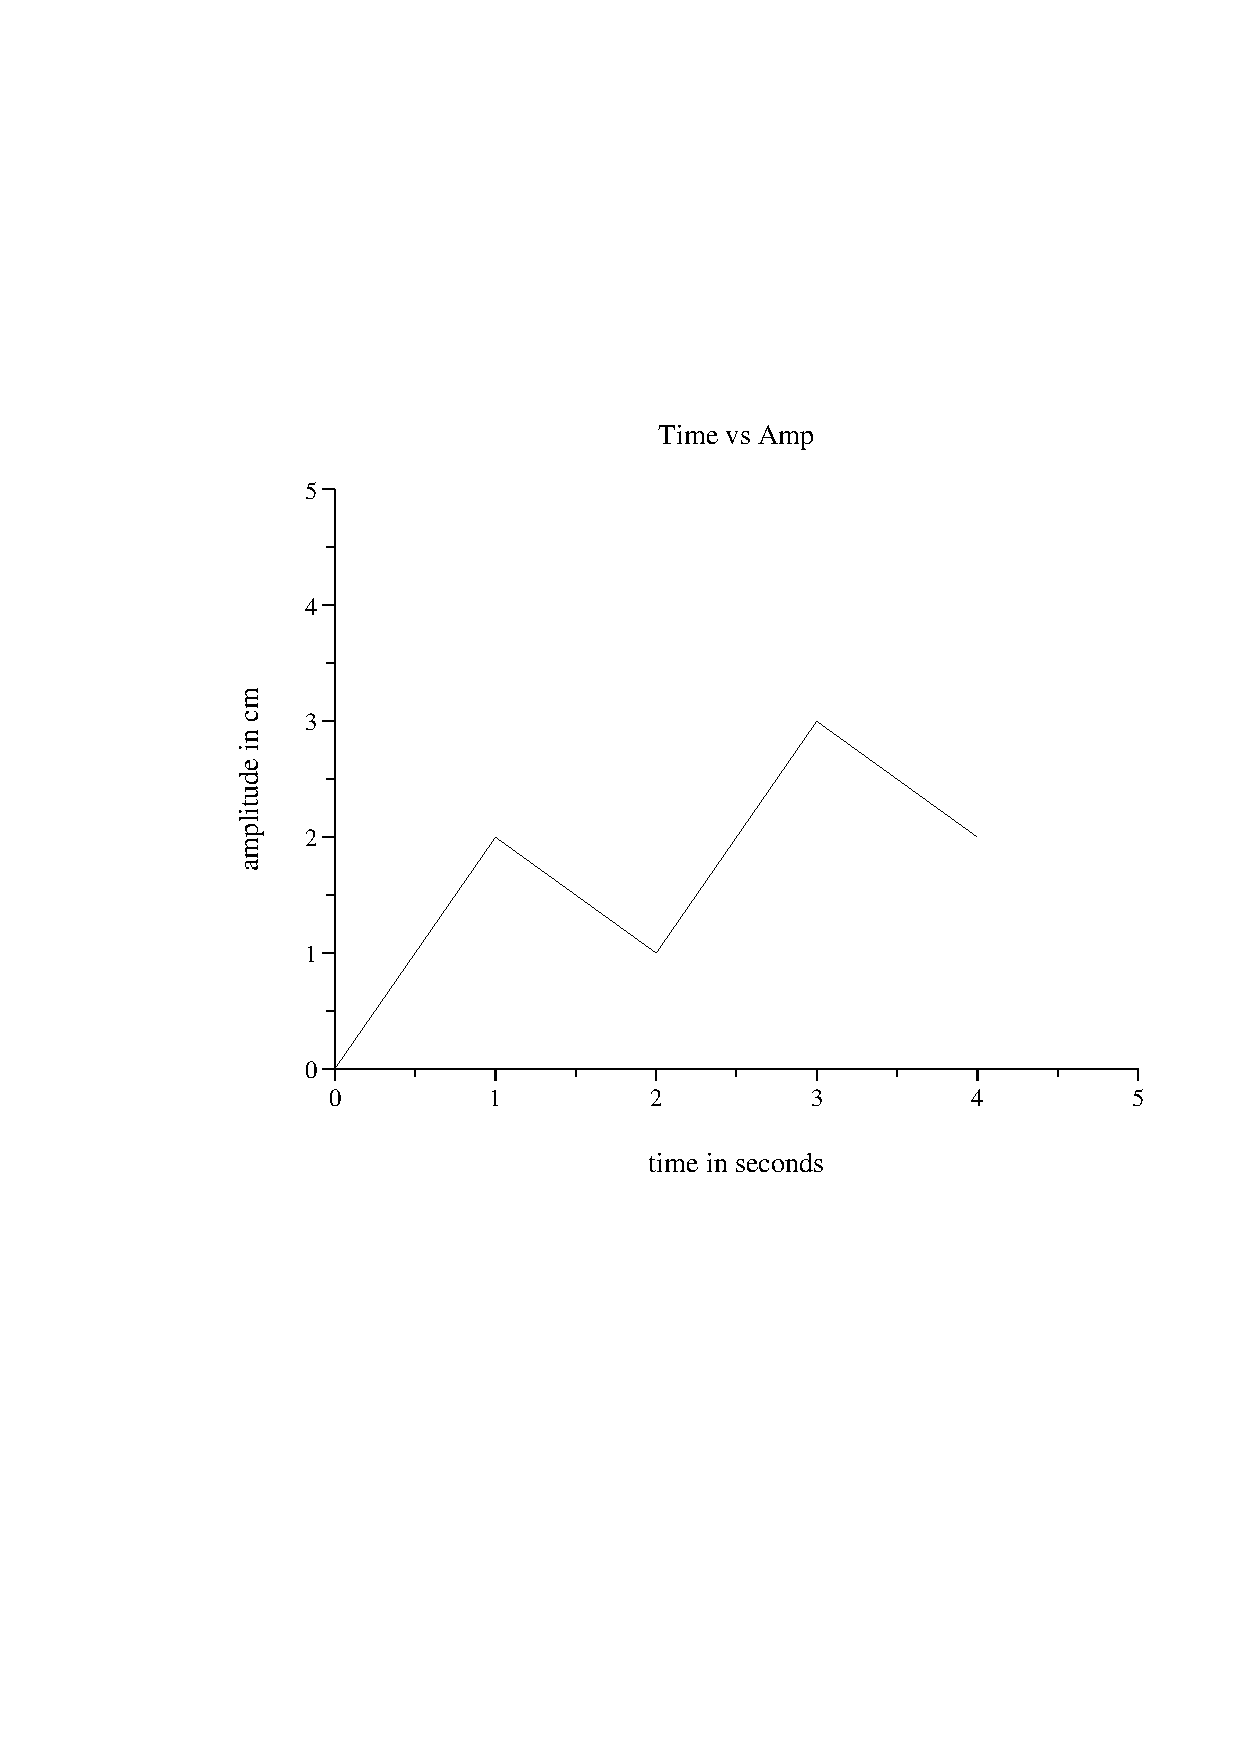
\epsfig{file=figure3,height=10cm}}
\end{center}

\begin{center}
\begin{boxedverbatim}

plt example1.data 0 2 -f example3.format\end{boxedverbatim}

\end{center}
\end{figure}%
\lthtmlfigureZ
\lthtmlcheckvsize\clearpage}

\stepcounter{section}
{\newpage\clearpage
\lthtmlfigureA{figure1063}%
\begin{figure}\begin{center}
\fcolorbox{blue}{white}{
\epsfig{file=henon,height=8cm}}
\end{center}
.
\end{figure}%
\lthtmlfigureZ
\lthtmlcheckvsize\clearpage}

\stepcounter{chapter}
{\newpage\clearpage
\lthtmlinlinemathA{tex2html_wrap_inline3655}%
$c$%
\lthtmlinlinemathZ
\lthtmlcheckvsize\clearpage}

{\newpage\clearpage
\lthtmlinlinemathA{tex2html_wrap_inline3679}%
$c-12$%
\lthtmlinlinemathZ
\lthtmlcheckvsize\clearpage}

{\newpage\clearpage
\lthtmlinlinemathA{tex2html_wrap_inline3683}%
$c-14$%
\lthtmlinlinemathZ
\lthtmlcheckvsize\clearpage}

{\newpage\clearpage
\lthtmlinlinemathA{tex2html_wrap_inline3703}%
$c-30$%
\lthtmlinlinemathZ
\lthtmlcheckvsize\clearpage}

{\newpage\clearpage
\lthtmlfigureA{figure1158}%
\begin{figure}\begin{center}
\begin{tabular}{p{10cm}p{1.5cm}}
\fcolorbox{blue}{white}{
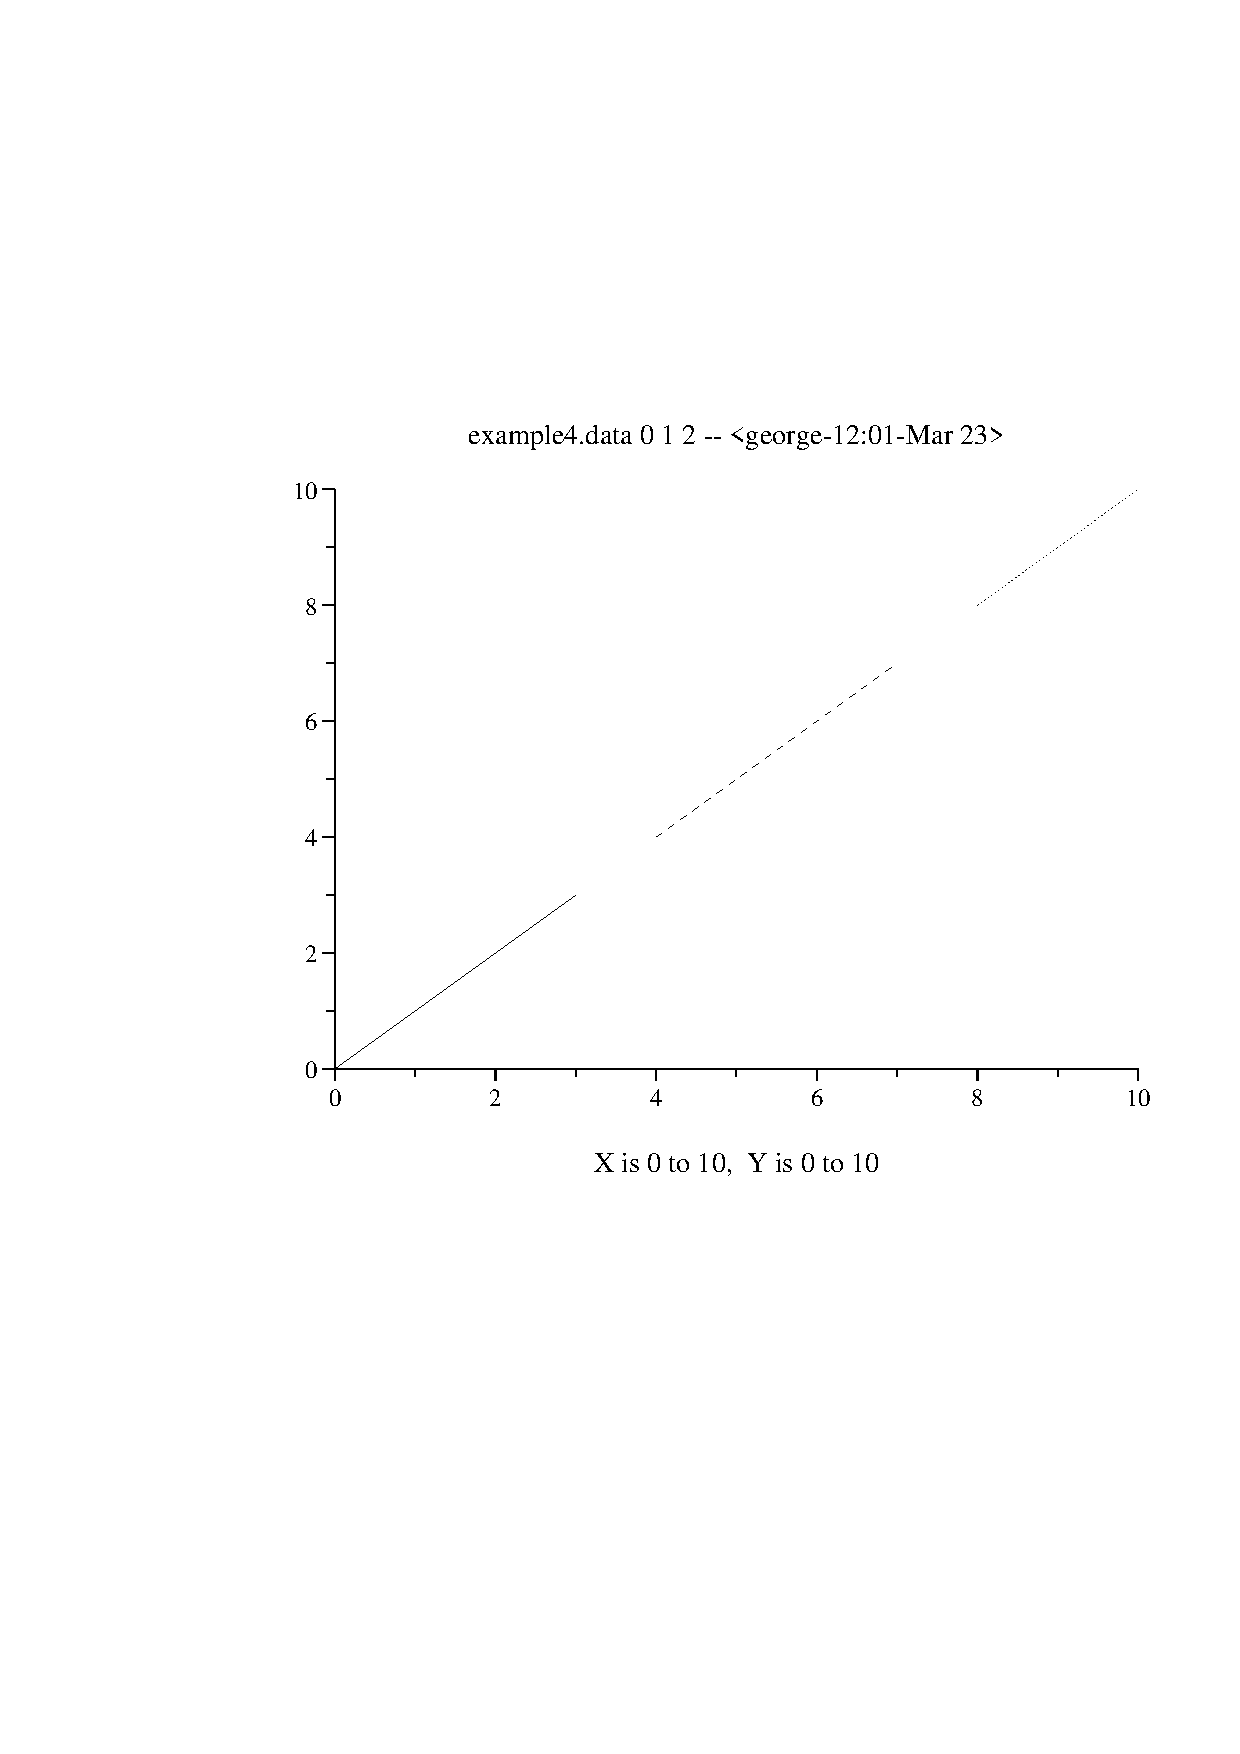
\epsfig{file=figure4,height=8cm}} &
{\vspace{-8cm}
{\em Data}
\vspace*{3mm}
\par
\begin{boxedverbatim}

0 0 0
3 3 0
1 7 23
4 4 0
7 7 0
2 6 23
8 8 0
10 10 0\end{boxedverbatim}

}
\end{tabular}
\end{center}

\begin{center}
\begin{boxedverbatim}

plt example4.data 0 1 2 -F"\
    fs helvetica longdashed dotted\
    p c"\end{boxedverbatim}

\end{center}
The two lines in the data file (at right, above) in which the third column
($c$) is 23 change the line styles to string $x$\  (the number specified in the
first column) from the fontgroup string array.  The fontgroup string array is
defined in the command line above (string 0 is ``{\tt helvetica}'', not used in
this example; string 1 is ``{\tt longdashed''}; and string 2 is ``{\tt
dotted}'').  Thus when {\tt plt} reads {\tt 1 7 23}, the line style changes
from the default (``{\tt solid}'') to the style specified by string 1 (``{tt
longdashed}''; the 7 is ignored), and when it reads {\tt 2 6 23}, the line
style becomes ``{\tt dotted}'' (and the 6 is similarly ignored).
\par
\hspace{2em}The line segments are not connected, because each non-zero $c$
value causes the previous segment to be drawn, and a new segment begins at the
next $(x,y)$\  pair.  If you wish to connect line segments in a plot such as
this, the input file must provide the segments' common endpoints twice, once
each before and after the line that changes {\tt plt}'s line style.
\end{figure}%
\lthtmlfigureZ
\lthtmlcheckvsize\clearpage}

{\newpage\clearpage
\lthtmlfigureA{figure1190}%
\begin{figure}\begin{center}
\fcolorbox{blue}{white}{
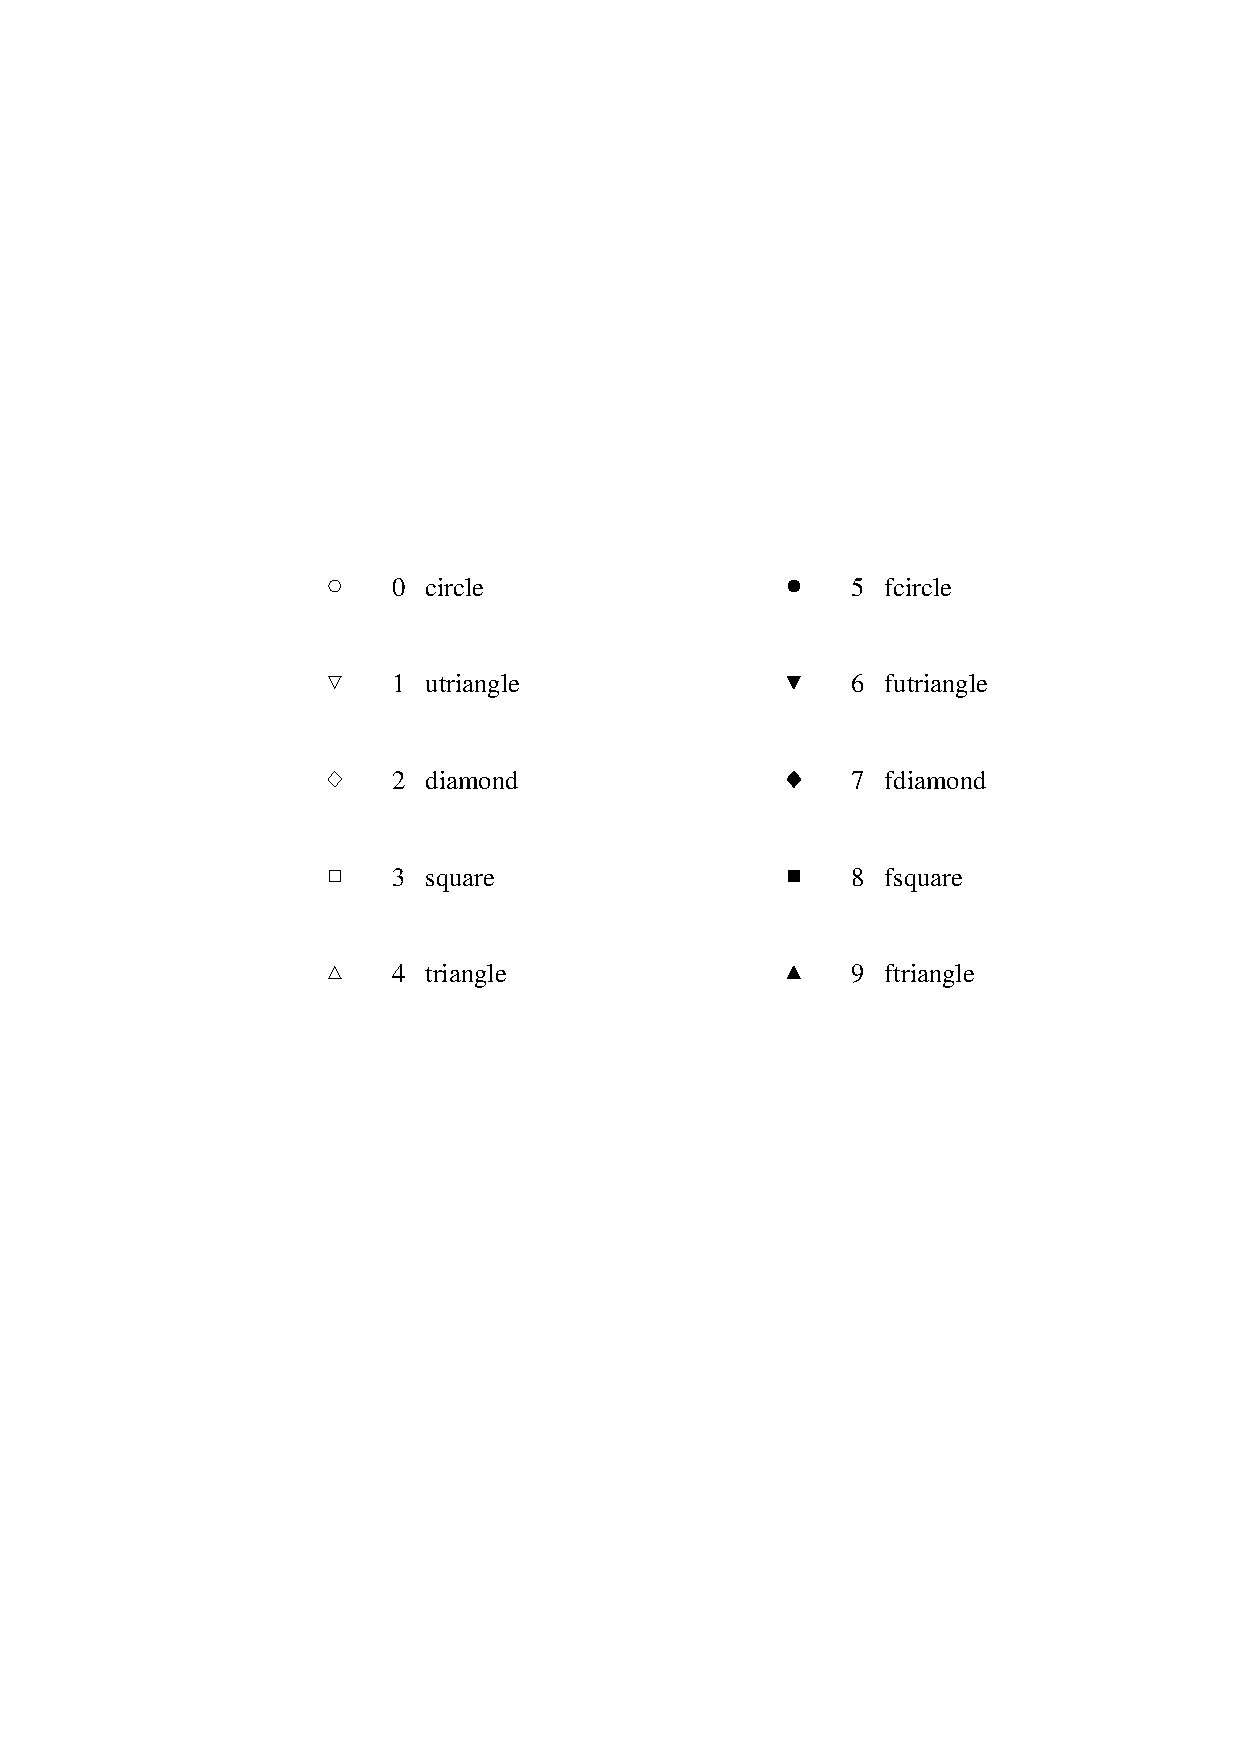
\epsfig{file=symbols,height=10cm}}
\end{center}

\end{figure}%
\lthtmlfigureZ
\lthtmlcheckvsize\clearpage}

{\newpage\clearpage
\lthtmlinlinemathA{tex2html_wrap_inline3727}%
$e$%
\lthtmlinlinemathZ
\lthtmlcheckvsize\clearpage}

{\newpage\clearpage
\lthtmlinlinemathA{tex2html_wrap_inline3761}%
$n$%
\lthtmlinlinemathZ
\lthtmlcheckvsize\clearpage}

{\newpage\clearpage
\lthtmlinlinemathA{tex2html_wrap_inline3777}%
$y_0$%
\lthtmlinlinemathZ
\lthtmlcheckvsize\clearpage}

{\newpage\clearpage
\lthtmlinlinemathA{tex2html_wrap_inline3779}%
$y_1$%
\lthtmlinlinemathZ
\lthtmlcheckvsize\clearpage}

{\newpage\clearpage
\lthtmlinlinemathA{tex2html_wrap_inline3781}%
$(x,y_0)$%
\lthtmlinlinemathZ
\lthtmlcheckvsize\clearpage}

{\newpage\clearpage
\lthtmlinlinemathA{tex2html_wrap_inline3783}%
$(x,y_1)$%
\lthtmlinlinemathZ
\lthtmlcheckvsize\clearpage}

{\newpage\clearpage
\lthtmlinlinemathA{tex2html_wrap_inline3791}%
$x_{0}$%
\lthtmlinlinemathZ
\lthtmlcheckvsize\clearpage}

{\newpage\clearpage
\lthtmlinlinemathA{tex2html_wrap_inline3793}%
$y_{0}$%
\lthtmlinlinemathZ
\lthtmlcheckvsize\clearpage}

{\newpage\clearpage
\lthtmlinlinemathA{tex2html_wrap_inline3795}%
$x_{1}$%
\lthtmlinlinemathZ
\lthtmlcheckvsize\clearpage}

{\newpage\clearpage
\lthtmlinlinemathA{tex2html_wrap_inline3797}%
$y_{1}$%
\lthtmlinlinemathZ
\lthtmlcheckvsize\clearpage}

{\newpage\clearpage
\lthtmlinlinemathA{tex2html_wrap_inline3799}%
$(x_{0},y_{0})$%
\lthtmlinlinemathZ
\lthtmlcheckvsize\clearpage}

{\newpage\clearpage
\lthtmlinlinemathA{tex2html_wrap_inline3801}%
$(x_{1},y_{1})$%
\lthtmlinlinemathZ
\lthtmlcheckvsize\clearpage}

\stepcounter{section}
{\newpage\clearpage
\lthtmlfigureA{figure1334}%
\begin{figure}\begin{center}
\fcolorbox{blue}{white}{
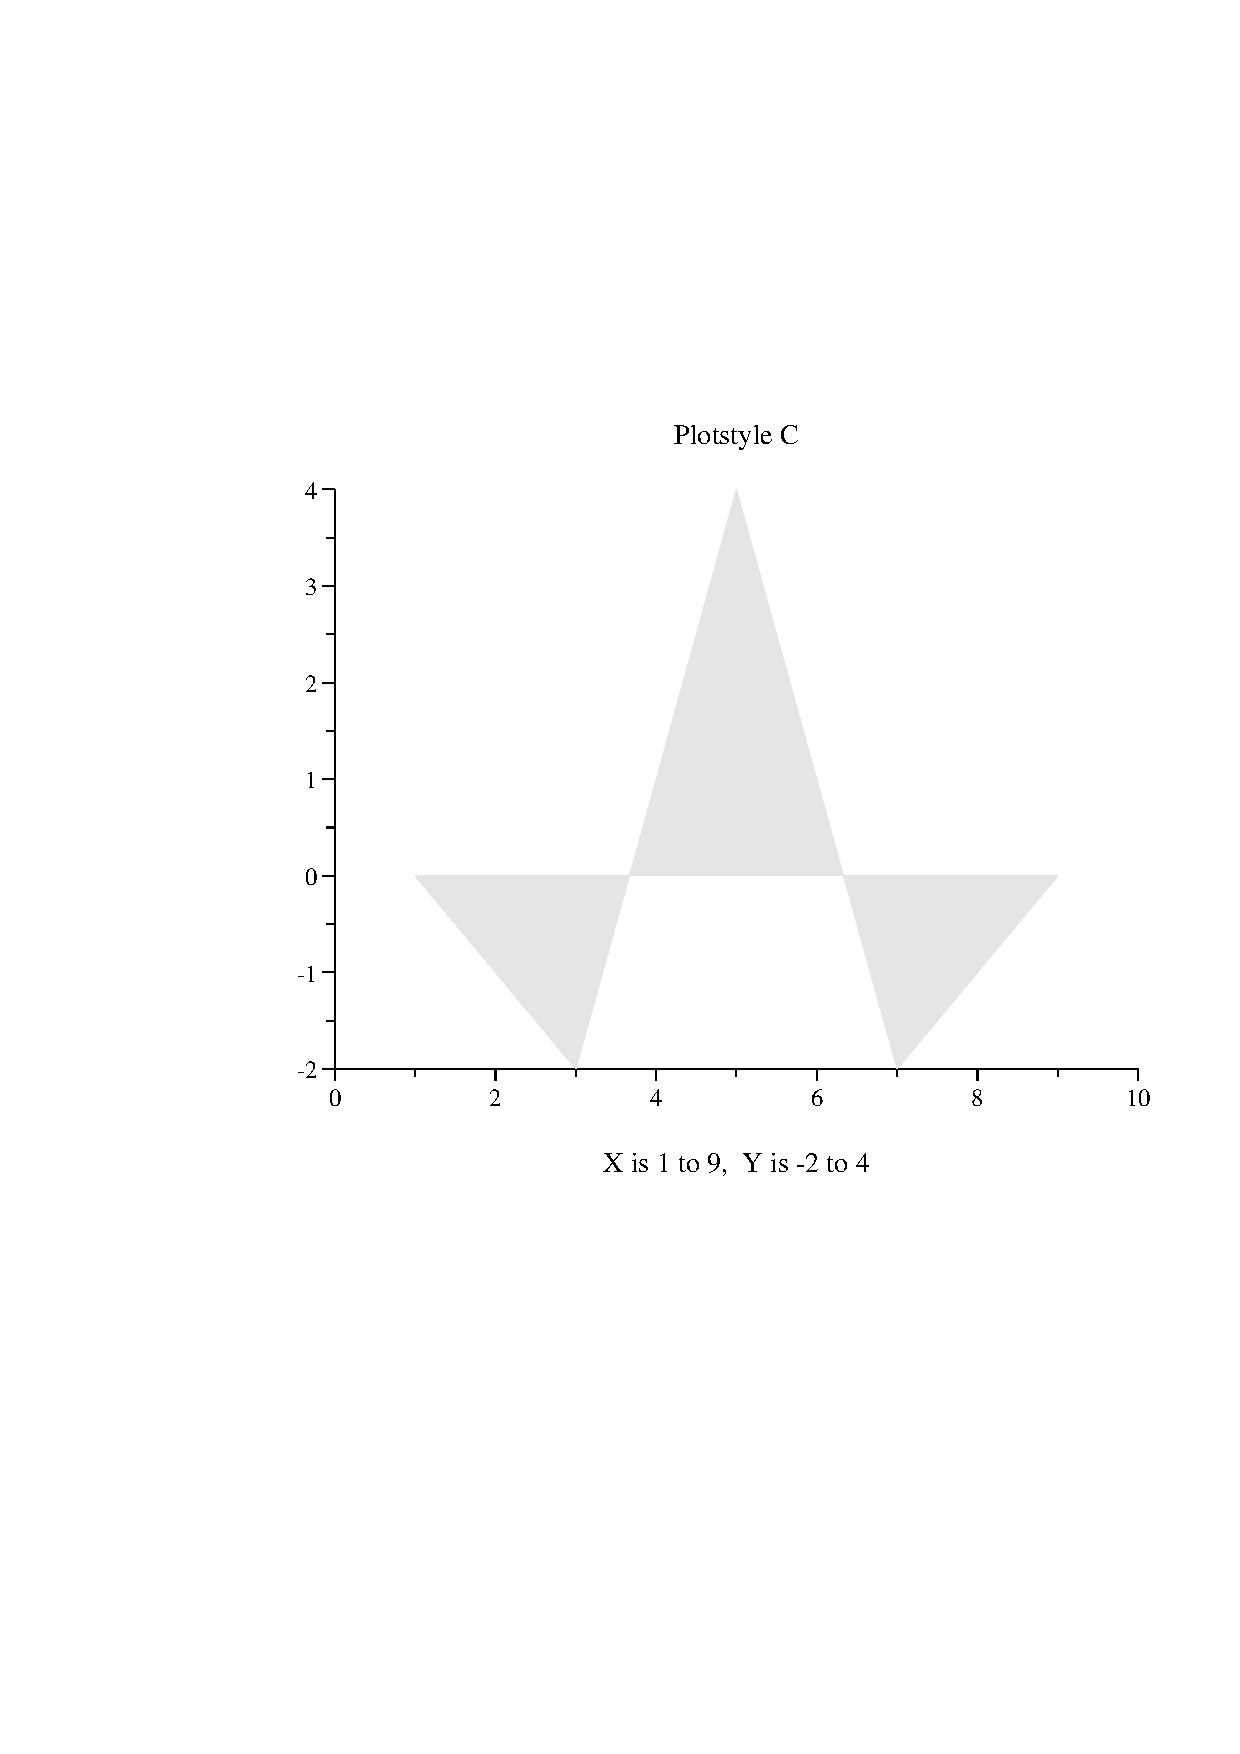
\epsfig{file=style-C,height=6.5cm}}
\end{center}

\begin{center}
\begin{boxedverbatim}

plt styles.data -p "0,1C(G.90)" -t "Plotstyle C"\end{boxedverbatim}

\end{center}
\end{figure}%
\lthtmlfigureZ
\lthtmlcheckvsize\clearpage}

{\newpage\clearpage
\lthtmlfigureA{figure1346}%
\begin{figure}\begin{center}
\fcolorbox{blue}{white}{
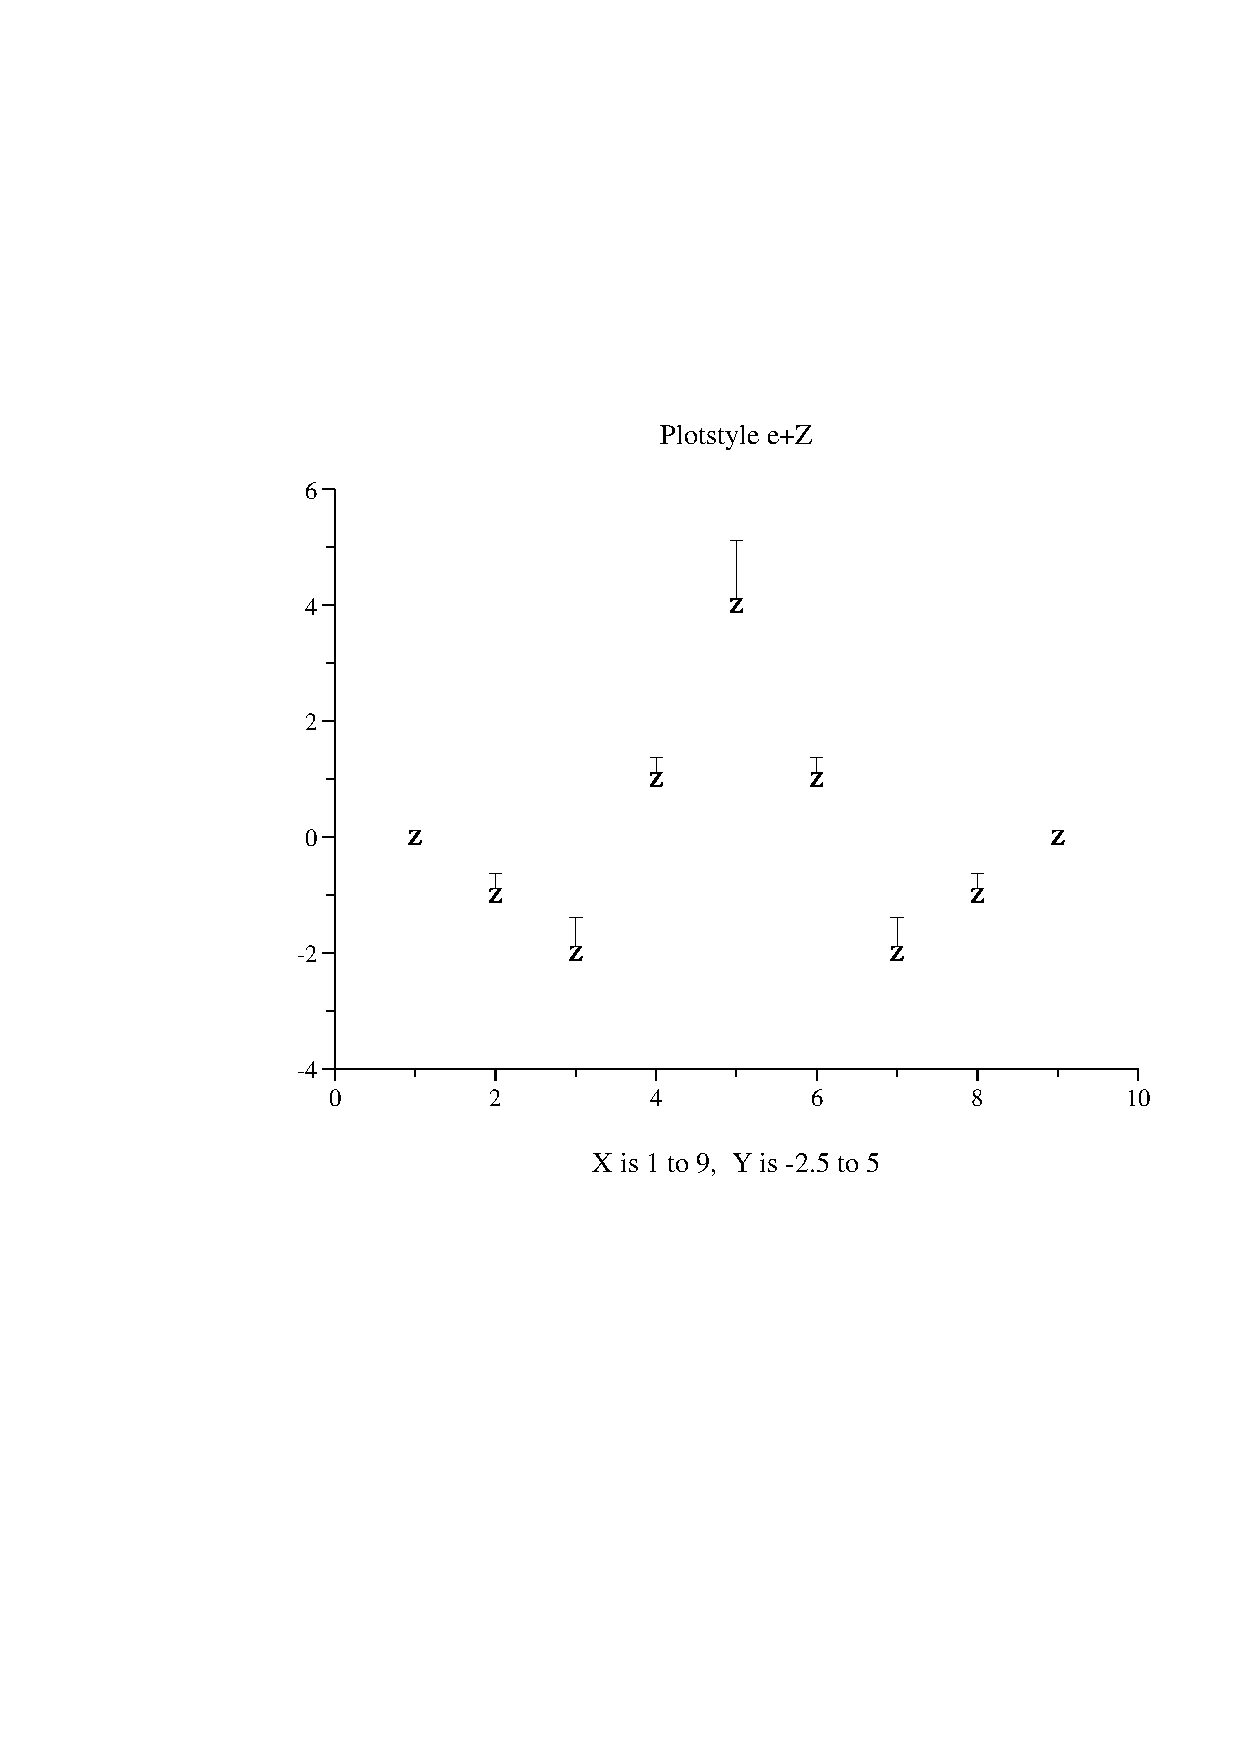
\epsfig{file=style-e+Z,height=6.5cm}}
\end{center}

\begin{center}
\begin{boxedverbatim}

plt styles.data -p 0,1,2e+Z -t "Plotstyle e+Z"\end{boxedverbatim}

\end{center}
\end{figure}%
\lthtmlfigureZ
\lthtmlcheckvsize\clearpage}

{\newpage\clearpage
\lthtmlfigureA{figure1358}%
\begin{figure}\begin{center}
\fcolorbox{blue}{white}{
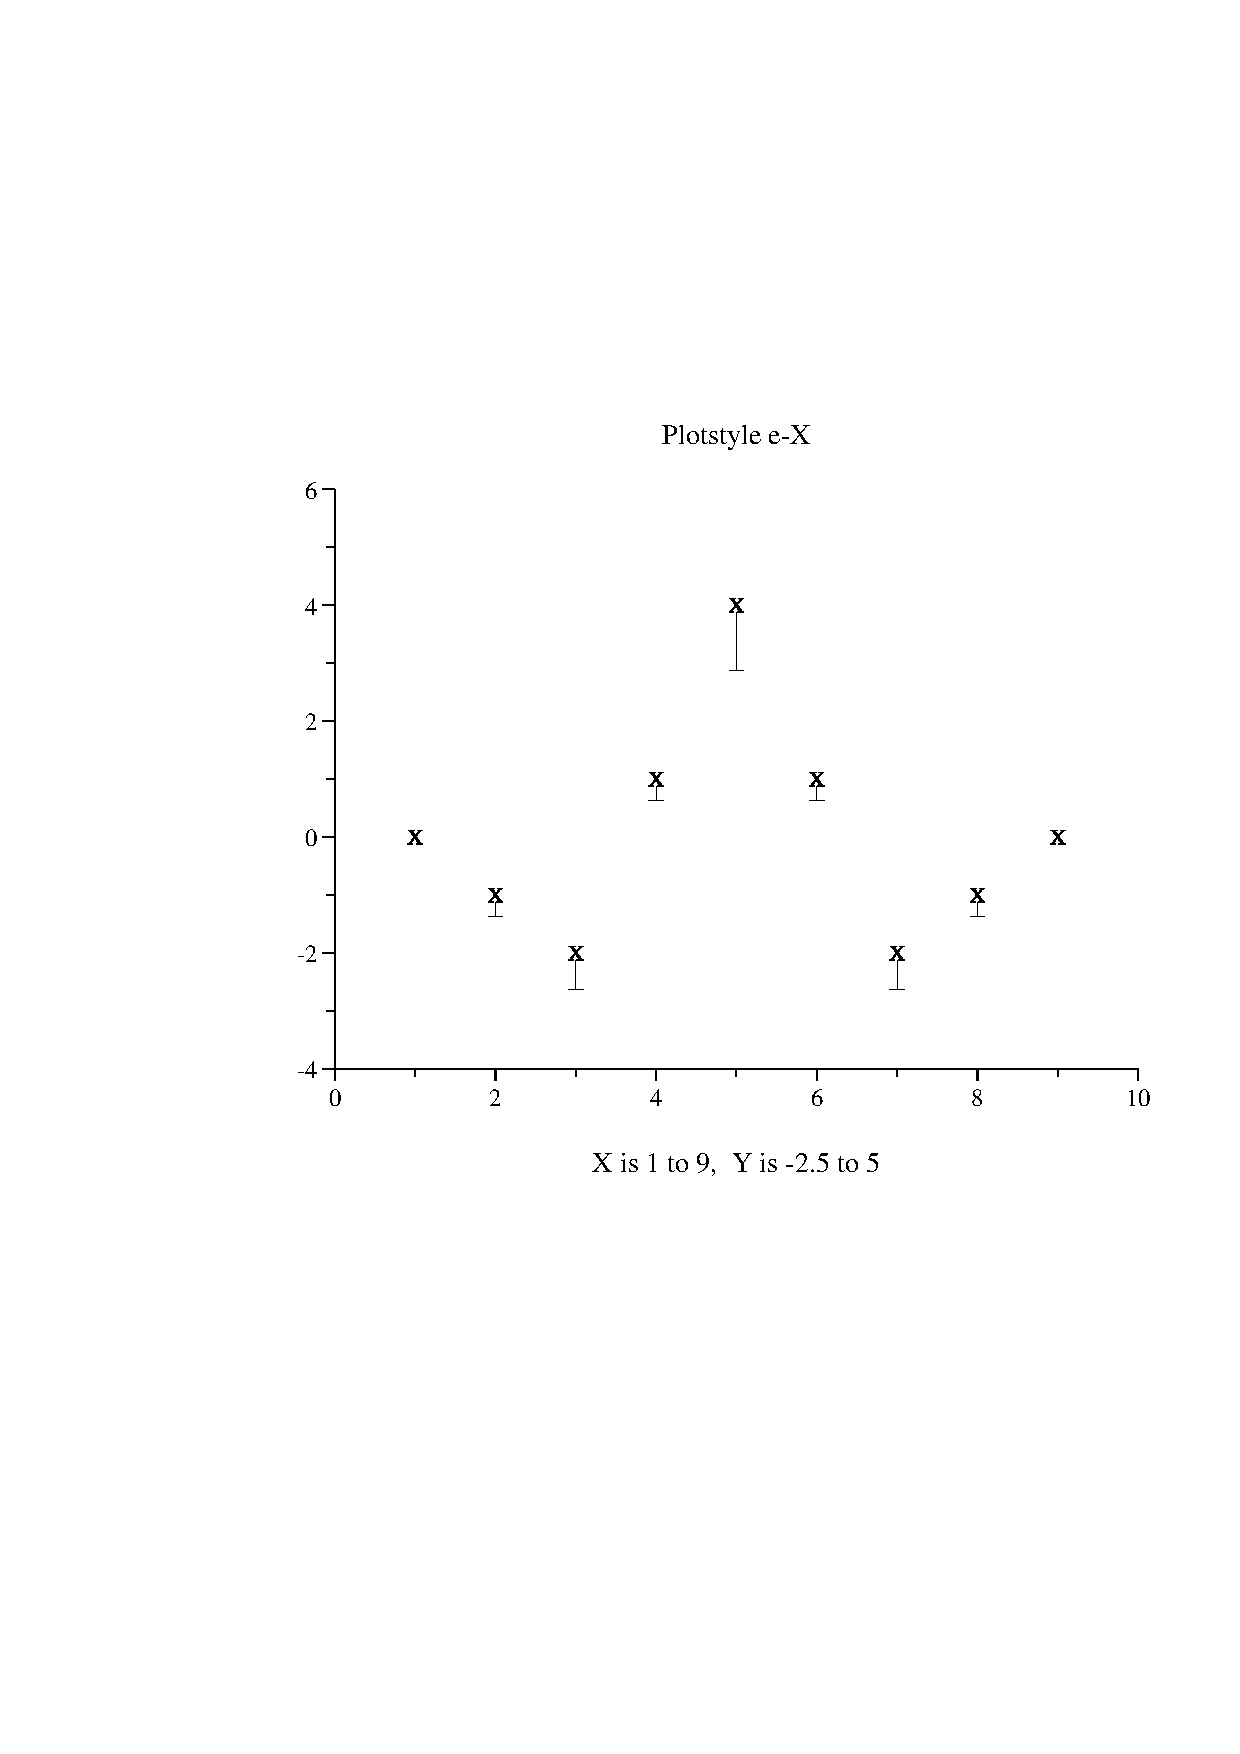
\epsfig{file=style-e-X,height=6.5cm}}
\end{center}

\begin{center}
\begin{boxedverbatim}

plt styles.data -p 0,1,2e-X -t "Plotstyle e-X"\end{boxedverbatim}

\end{center}
\end{figure}%
\lthtmlfigureZ
\lthtmlcheckvsize\clearpage}

{\newpage\clearpage
\lthtmlfigureA{figure1370}%
\begin{figure}\begin{center}
\fcolorbox{blue}{white}{
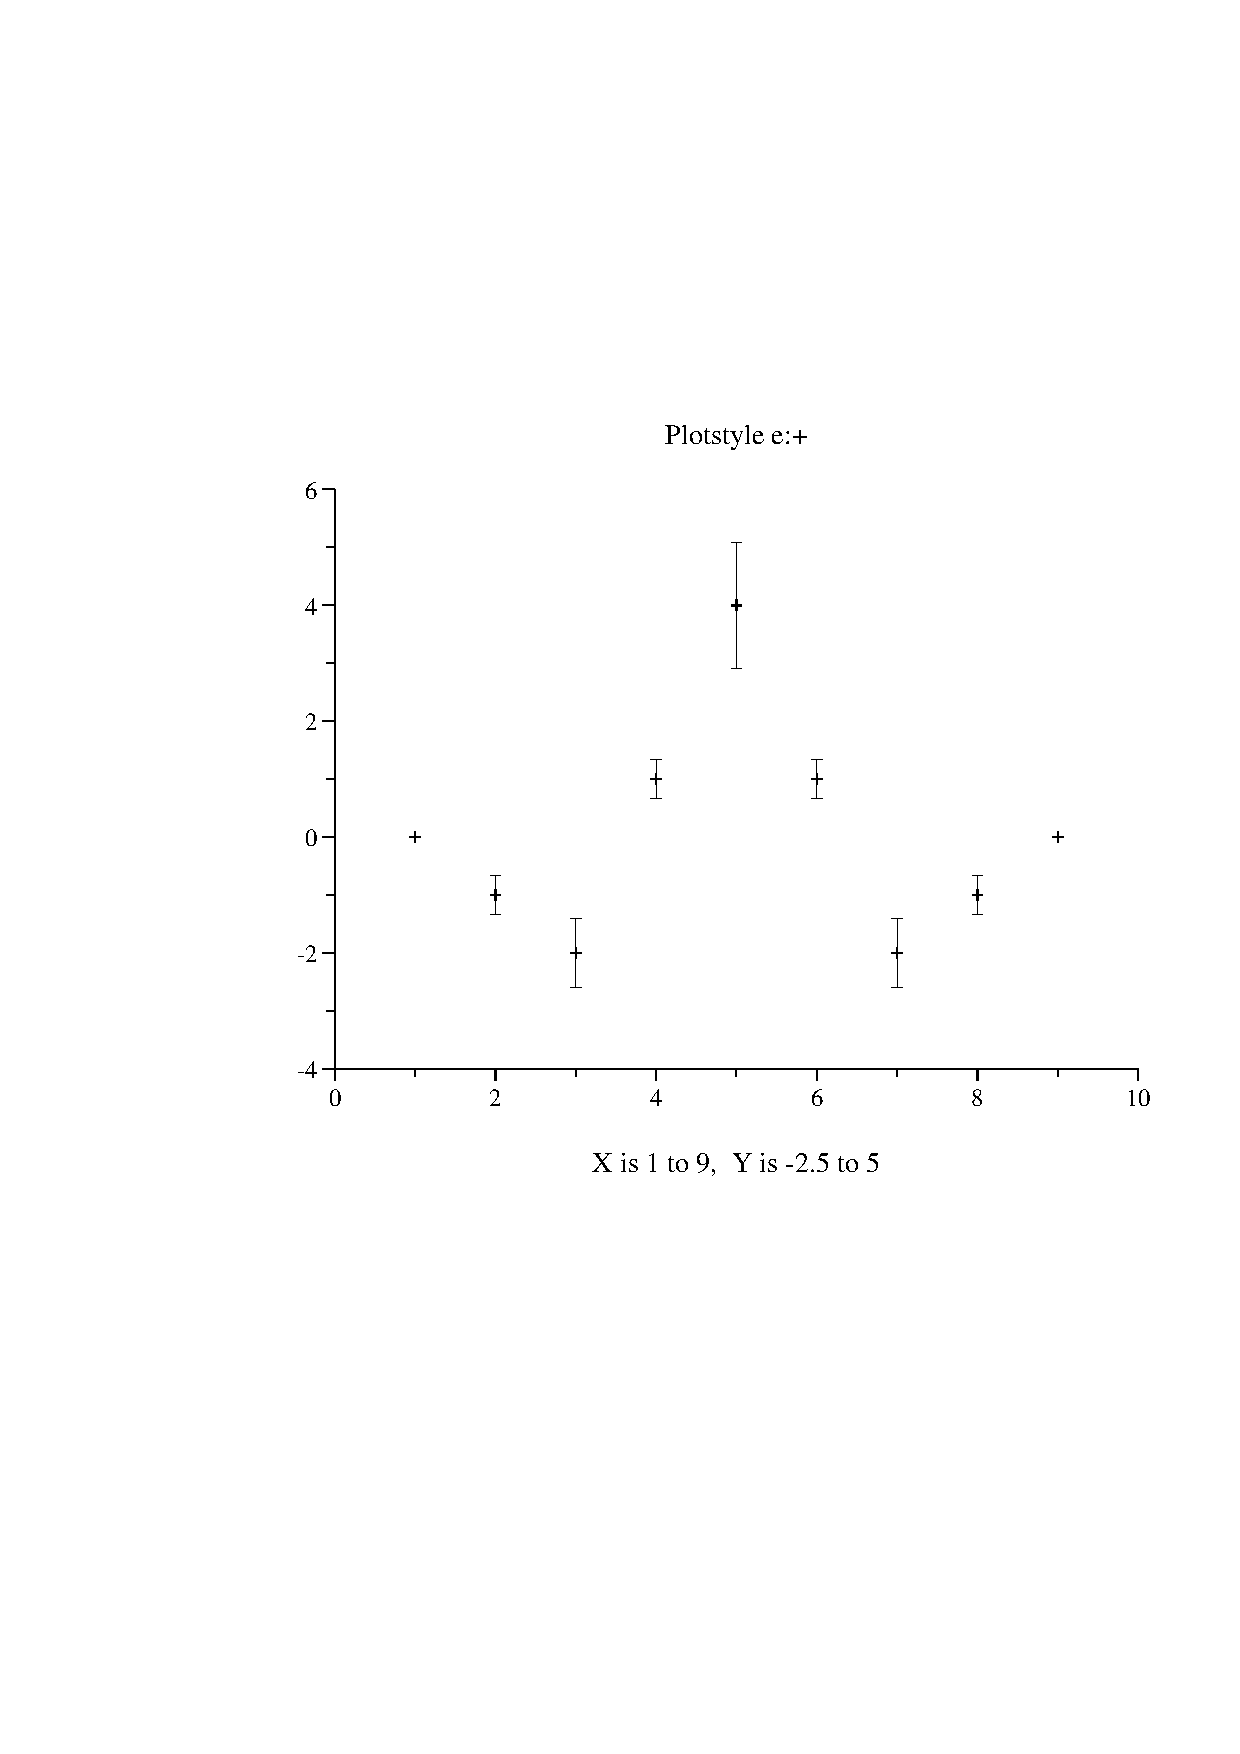
\epsfig{file=style-ec+,height=6.5cm}}
\end{center}

\begin{center}
\begin{boxedverbatim}

plt styles.data -p 0,1,2e:+ -t "Plotstyle e:+"\end{boxedverbatim}

\end{center}
\end{figure}%
\lthtmlfigureZ
\lthtmlcheckvsize\clearpage}

{\newpage\clearpage
\lthtmlfigureA{figure1382}%
\begin{figure}\begin{center}
\fcolorbox{blue}{white}{
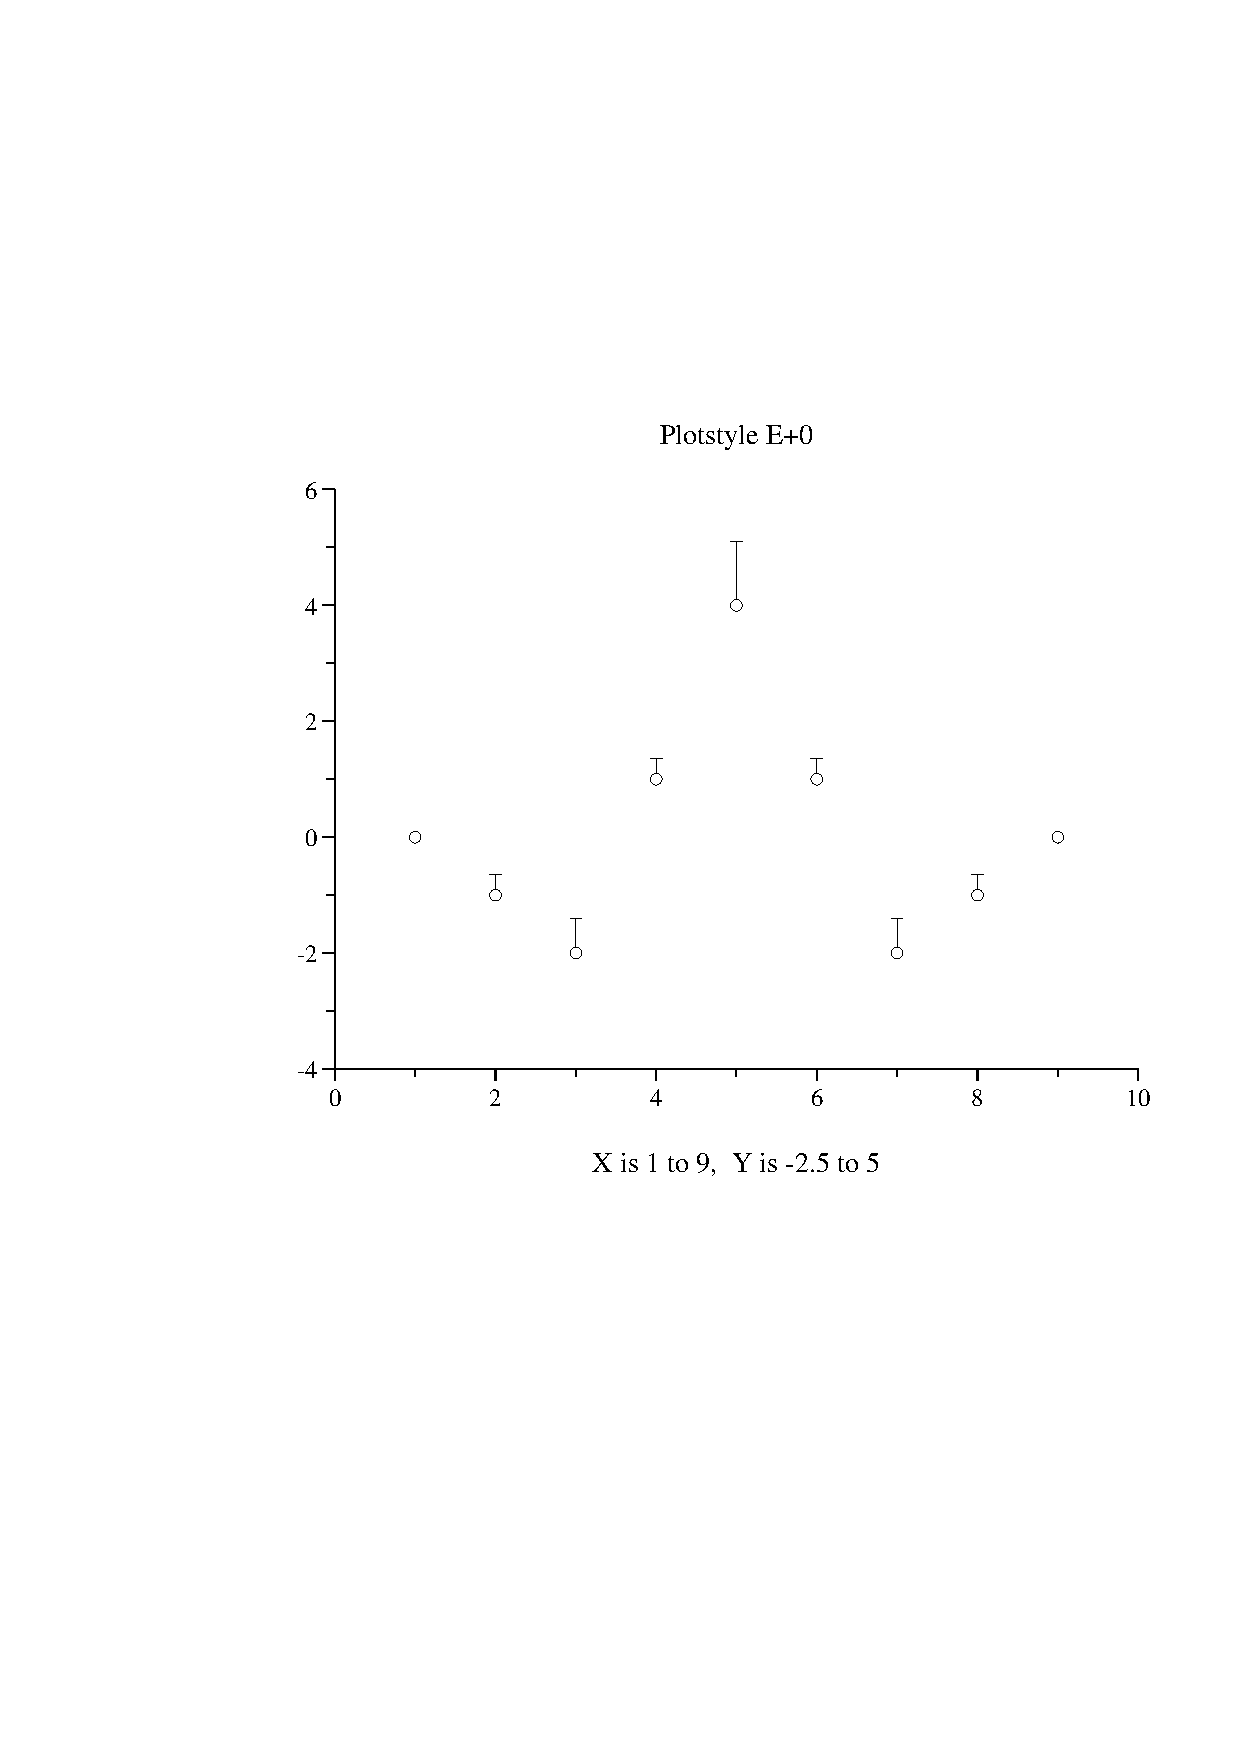
\epsfig{file=style-E+0,height=6.5cm}}
\end{center}

\begin{center}
\begin{boxedverbatim}

plt styles.data -p 0,1,2E+0 -t "Plotstyle E+0"\end{boxedverbatim}

\end{center}
\end{figure}%
\lthtmlfigureZ
\lthtmlcheckvsize\clearpage}

{\newpage\clearpage
\lthtmlfigureA{figure1394}%
\begin{figure}\begin{center}
\fcolorbox{blue}{white}{
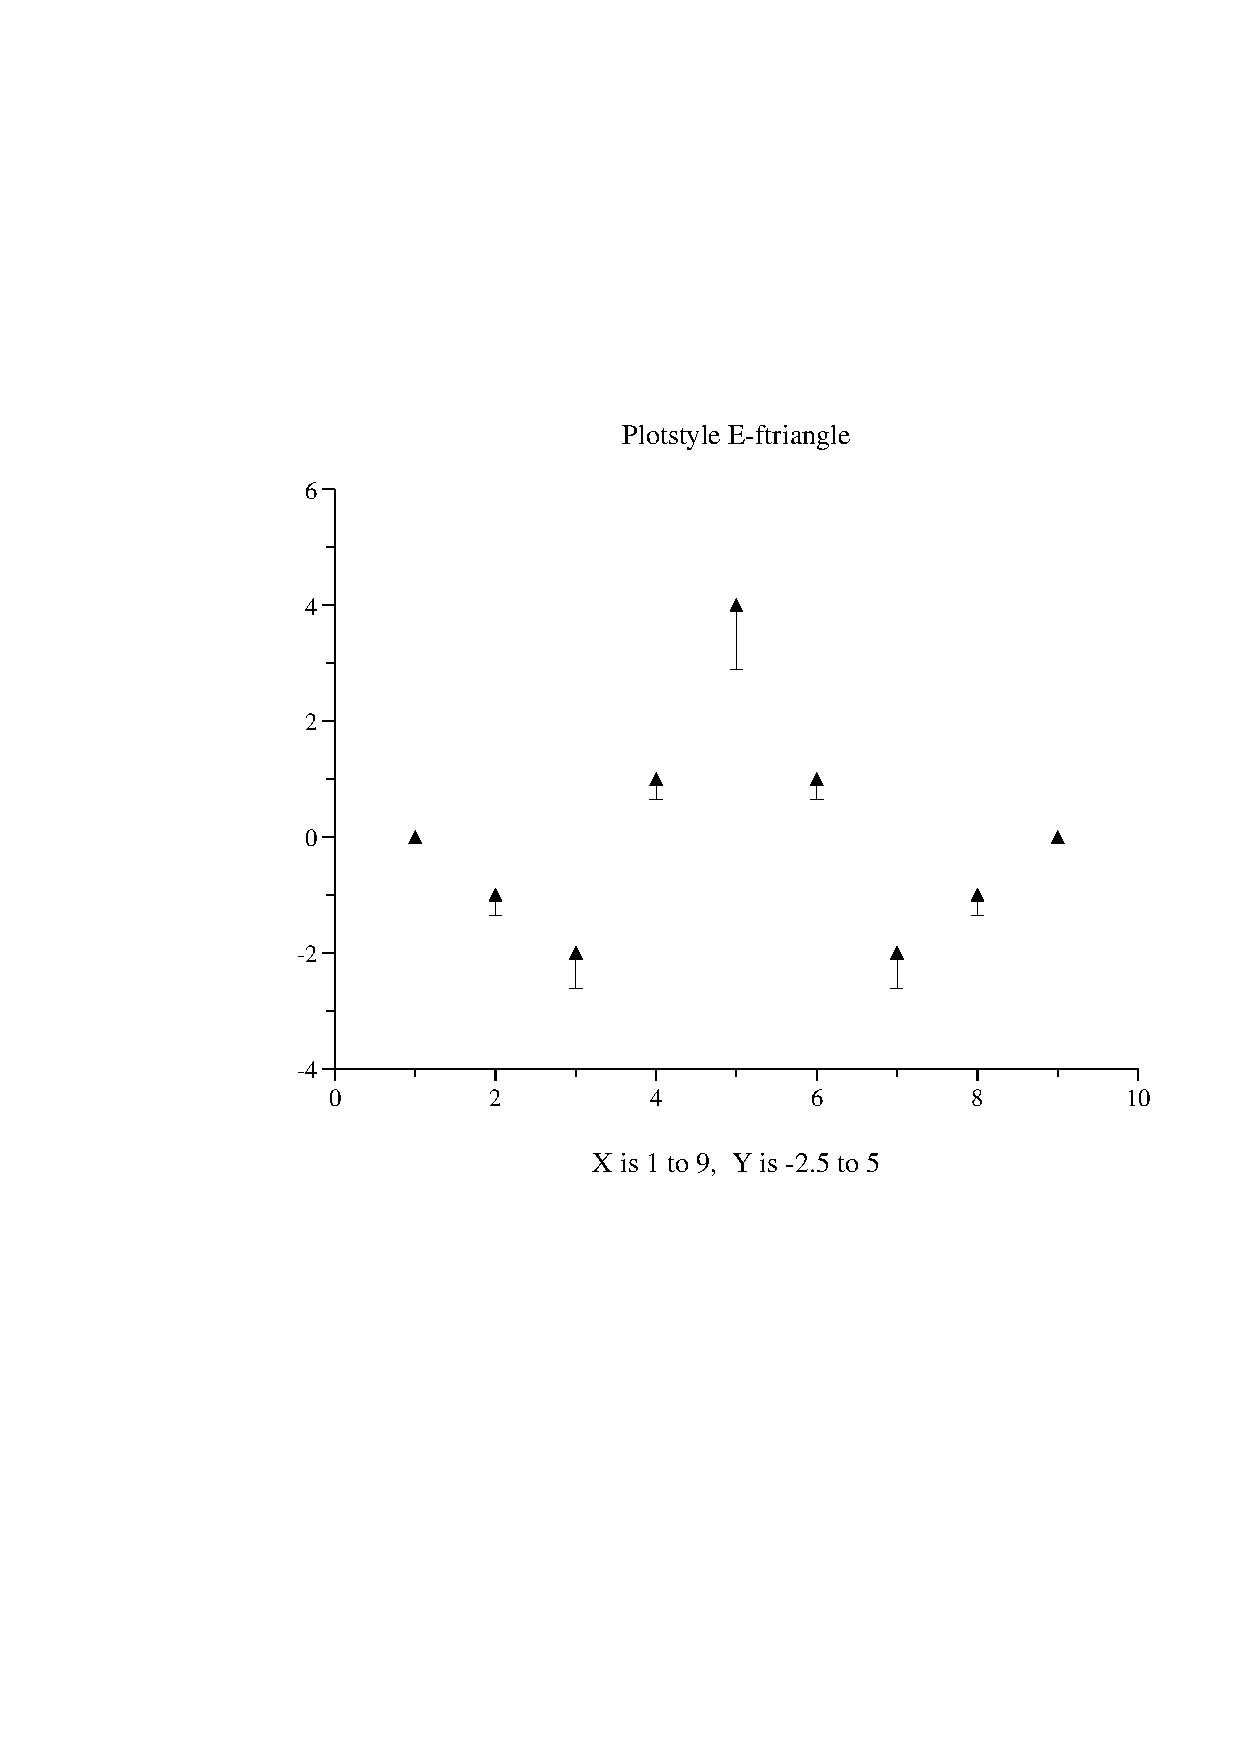
\epsfig{file=style-E-ftriangle,height=6.5cm}}
\end{center}

\begin{center}
\begin{boxedverbatim}

plt styles.data -p 0,1,2E-ftriangle -t "Plotstyle E-ftriangle"\end{boxedverbatim}

\end{center}
\end{figure}%
\lthtmlfigureZ
\lthtmlcheckvsize\clearpage}

{\newpage\clearpage
\lthtmlfigureA{figure1406}%
\begin{figure}\begin{center}
\fcolorbox{blue}{white}{
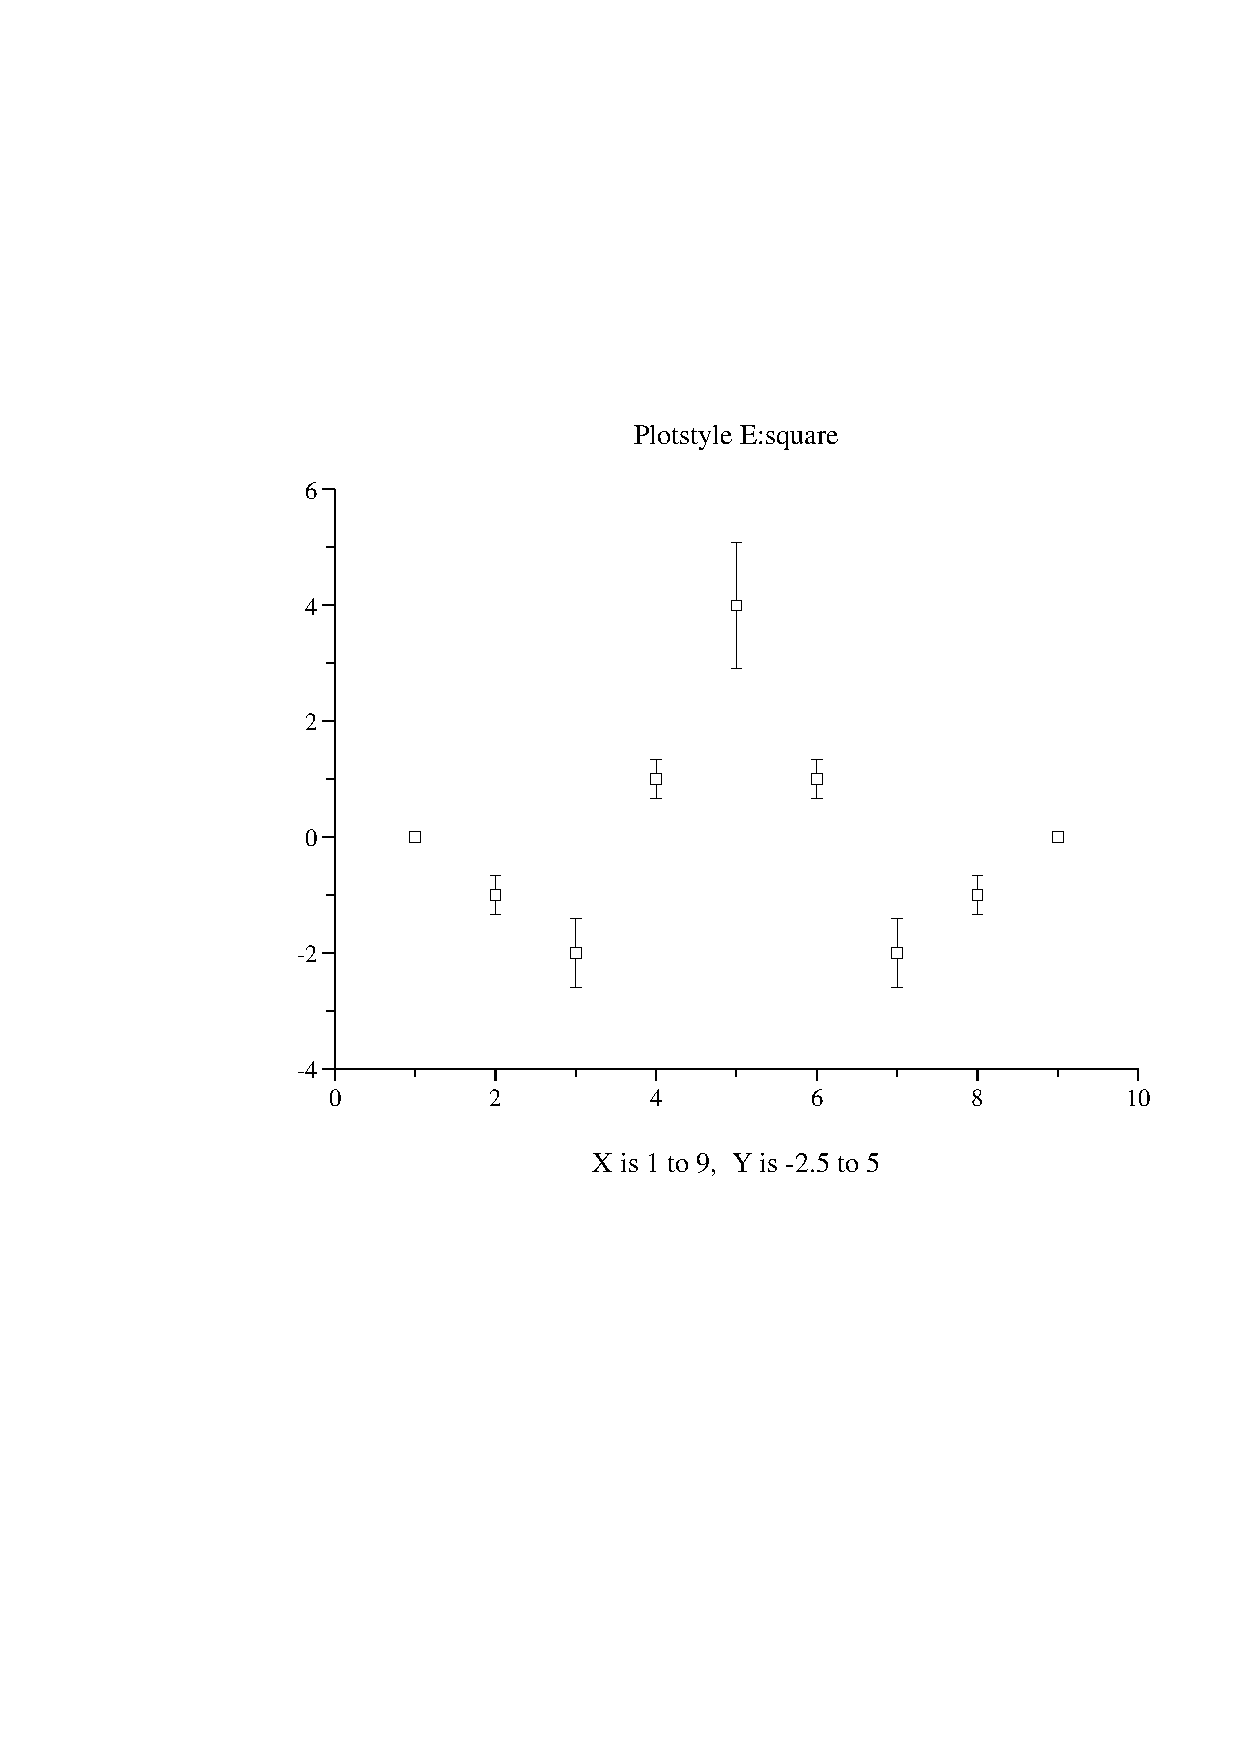
\epsfig{file=style-Ecsquare,height=6.5cm}}
\end{center}

\begin{center}
\begin{boxedverbatim}

plt styles.data -p 0,1,2E:square -t "Plotstyle E:square"\end{boxedverbatim}

\end{center}
\end{figure}%
\lthtmlfigureZ
\lthtmlcheckvsize\clearpage}

{\newpage\clearpage
\lthtmlfigureA{figure1418}%
\begin{figure}\begin{center}
\fcolorbox{blue}{white}{
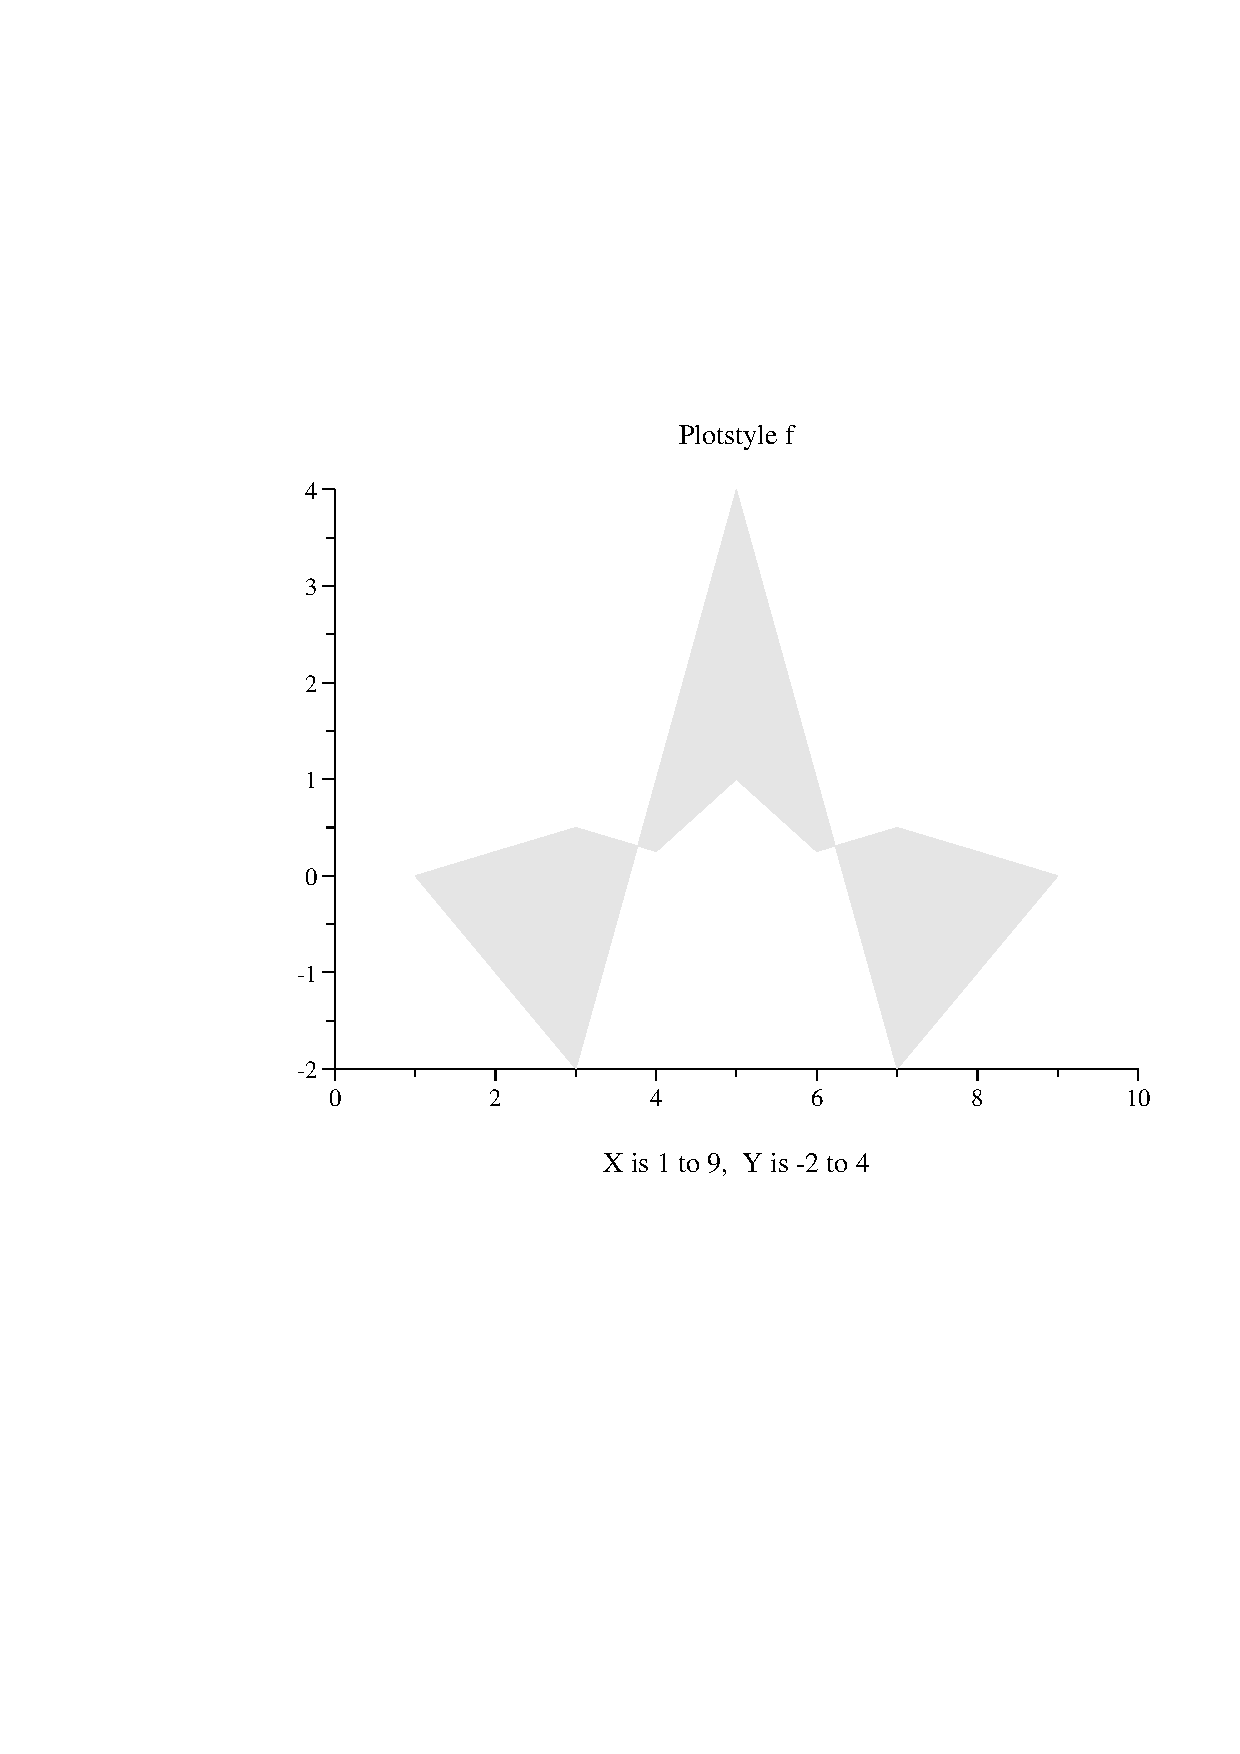
\epsfig{file=style-f,height=6.5cm}}
\end{center}

\begin{center}
\begin{boxedverbatim}

plt styles.data -p "0,1,2f(G.90)" -t "Plotstyle f"\end{boxedverbatim}

\end{center}
\end{figure}%
\lthtmlfigureZ
\lthtmlcheckvsize\clearpage}

{\newpage\clearpage
\lthtmlfigureA{figure1430}%
\begin{figure}\begin{center}
\fcolorbox{blue}{white}{
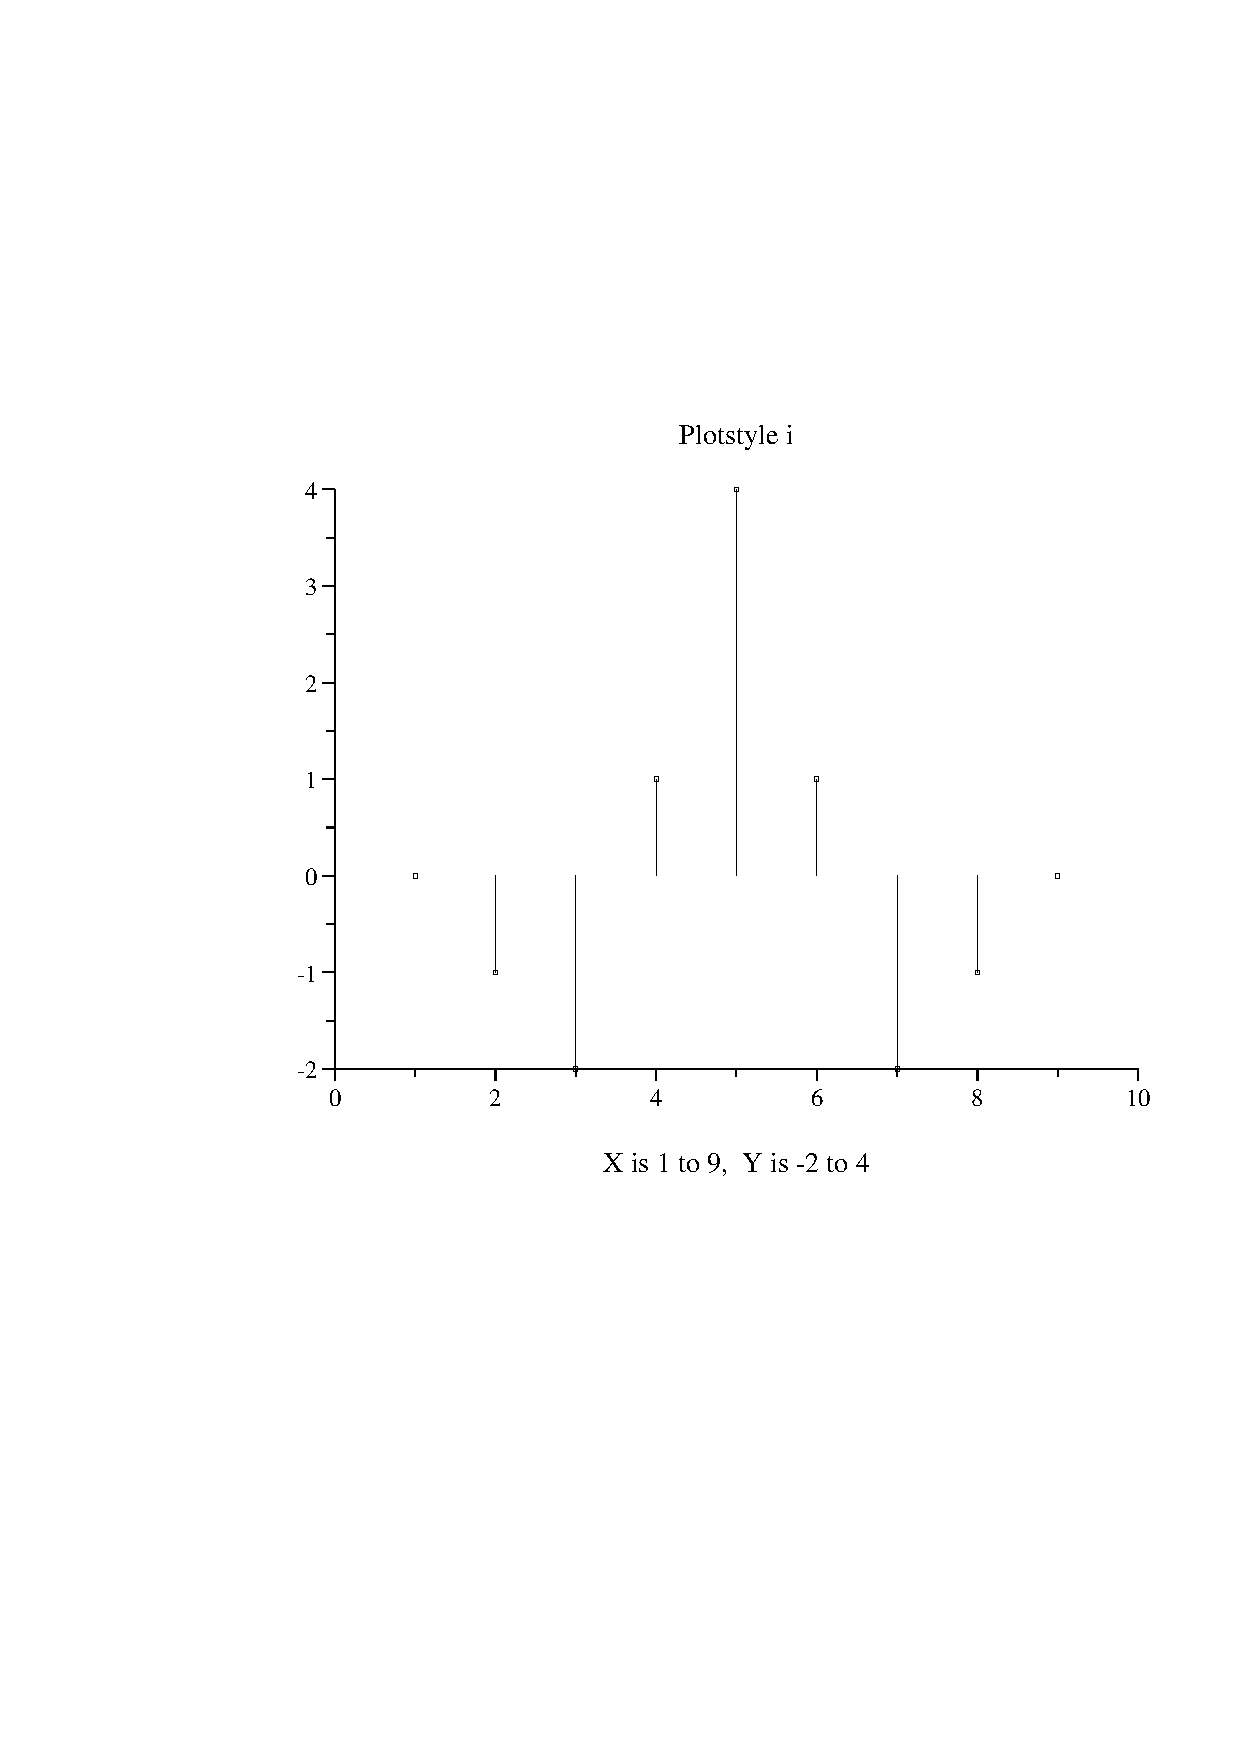
\epsfig{file=style-i,height=6.5cm}}
\end{center}

\begin{center}
\begin{boxedverbatim}

plt styles.data -p 0,1i -t "Plotstyle i"\end{boxedverbatim}

\end{center}
\end{figure}%
\lthtmlfigureZ
\lthtmlcheckvsize\clearpage}

{\newpage\clearpage
\lthtmlfigureA{figure1442}%
\begin{figure}\begin{center}
\fcolorbox{blue}{white}{
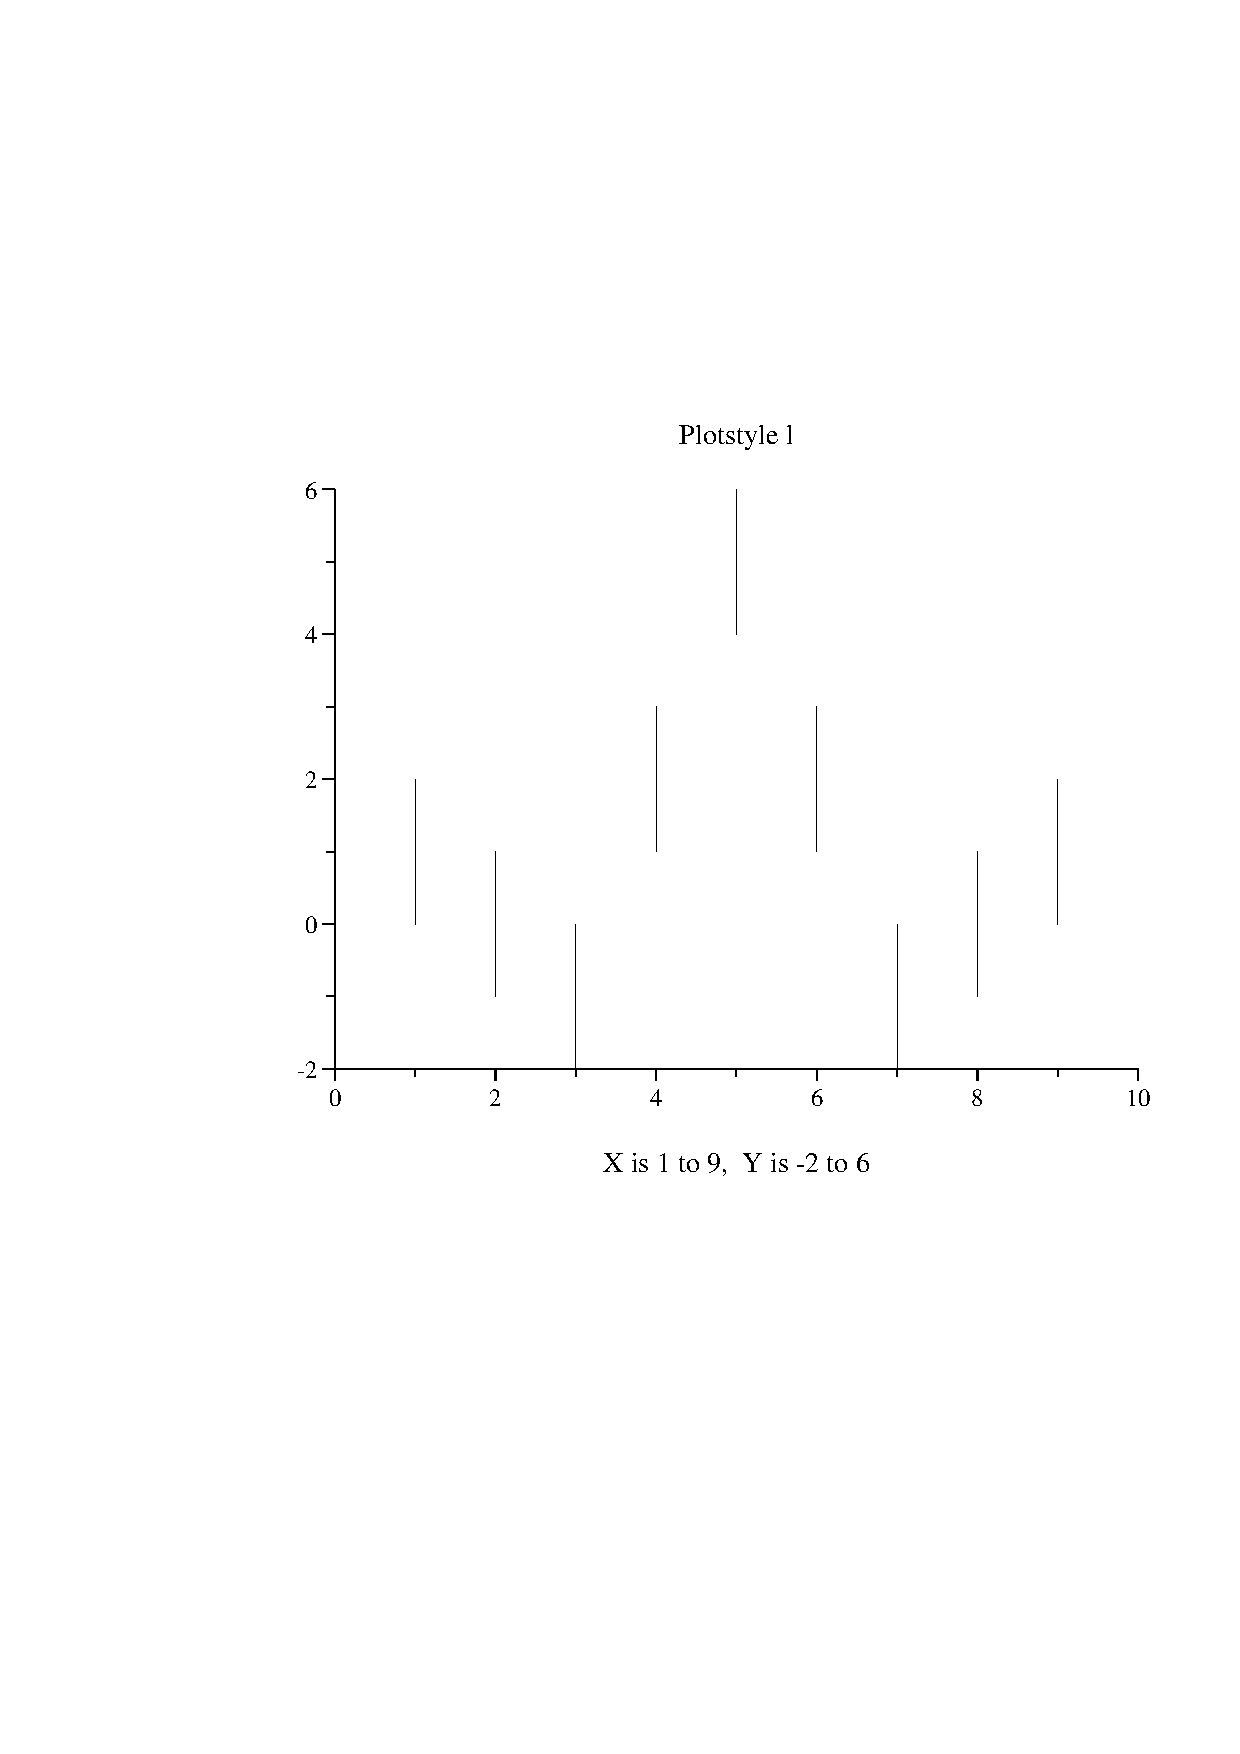
\epsfig{file=style-l,height=6.5cm}}
\end{center}

\begin{center}
\begin{boxedverbatim}

plt styles.data -p 0,1,0,3l -t "Plotstyle l"\end{boxedverbatim}

\end{center}
\end{figure}%
\lthtmlfigureZ
\lthtmlcheckvsize\clearpage}

{\newpage\clearpage
\lthtmlfigureA{figure1454}%
\begin{figure}\begin{center}
\fcolorbox{blue}{white}{
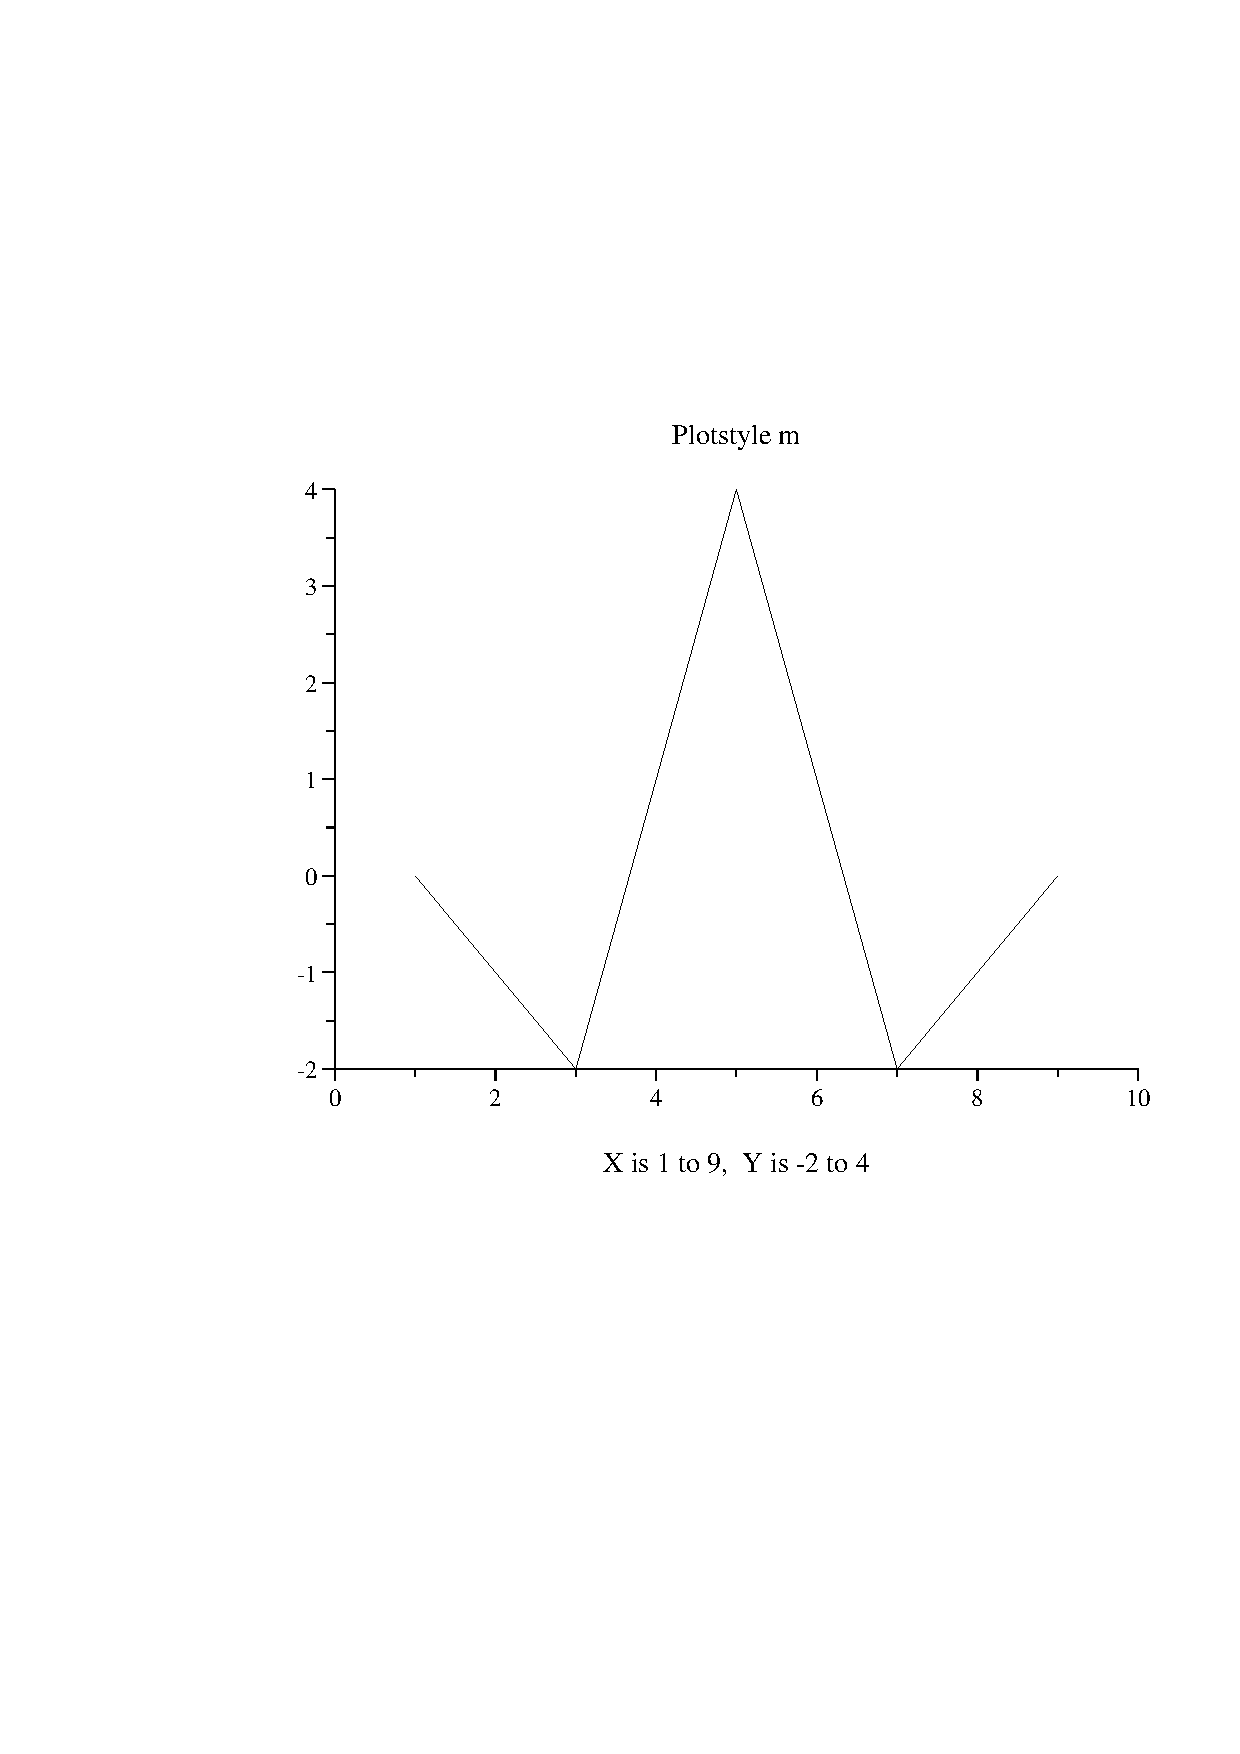
\epsfig{file=style-m,height=6.5cm}}
\end{center}

\begin{center}
\begin{boxedverbatim}

plt styles.data -p 1m -t "Plotstyle m"\end{boxedverbatim}

\end{center}
\end{figure}%
\lthtmlfigureZ
\lthtmlcheckvsize\clearpage}

{\newpage\clearpage
\lthtmlfigureA{figure1466}%
\begin{figure}\begin{center}
\fcolorbox{blue}{white}{
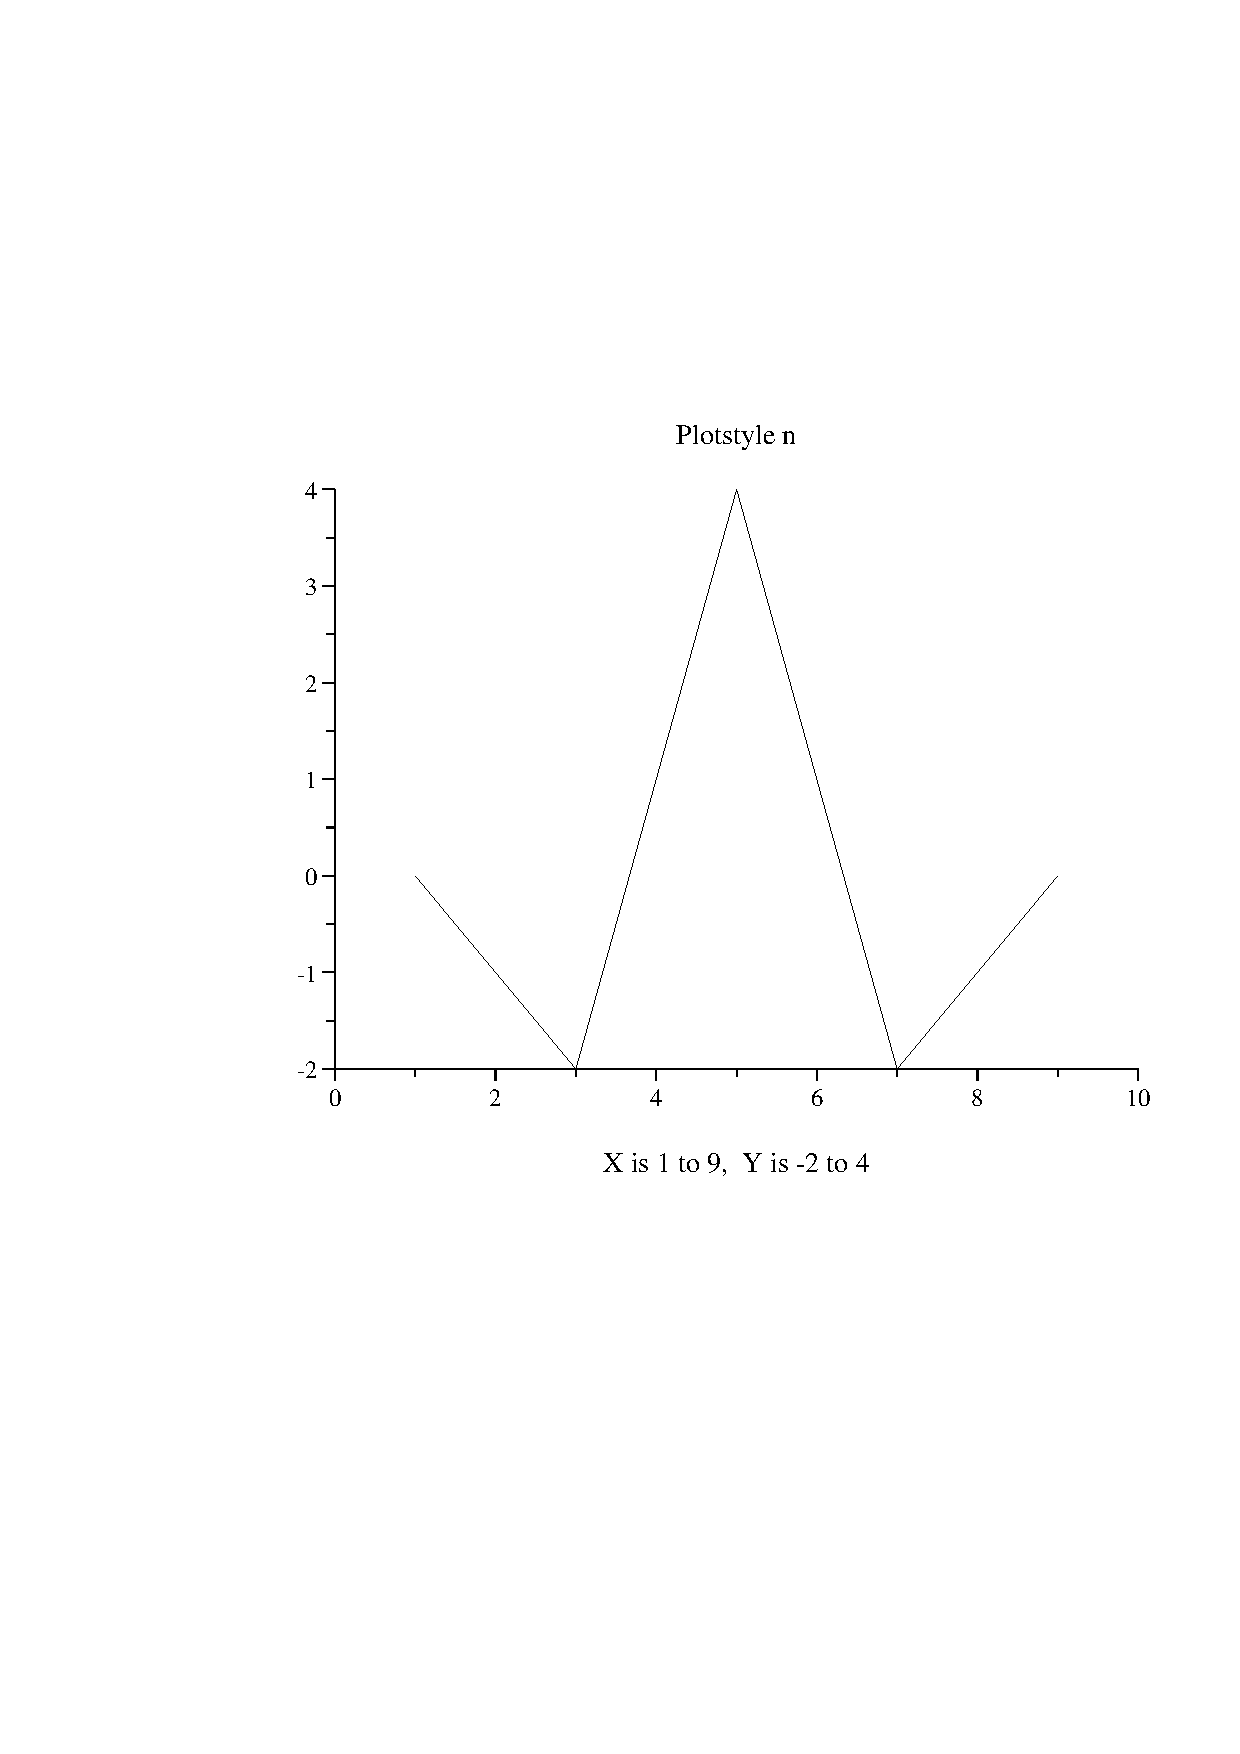
\epsfig{file=style-n,height=6.5cm}}
\end{center}

\begin{center}
\begin{boxedverbatim}

plt styles.data -p 0,1n -t "Plotstyle n"\end{boxedverbatim}

\end{center}
\end{figure}%
\lthtmlfigureZ
\lthtmlcheckvsize\clearpage}

{\newpage\clearpage
\lthtmlfigureA{figure1478}%
\begin{figure}\begin{center}
\fcolorbox{blue}{white}{
\epsfig{file=style-N,height=6.5cm}}
\end{center}

\begin{center}
\begin{boxedverbatim}

plt styles.data -p "0,1N(G.90)" -t "Plotstyle N"\end{boxedverbatim}

\end{center}
\end{figure}%
\lthtmlfigureZ
\lthtmlcheckvsize\clearpage}

{\newpage\clearpage
\lthtmlfigureA{figure1490}%
\begin{figure}\begin{center}
\fcolorbox{blue}{white}{
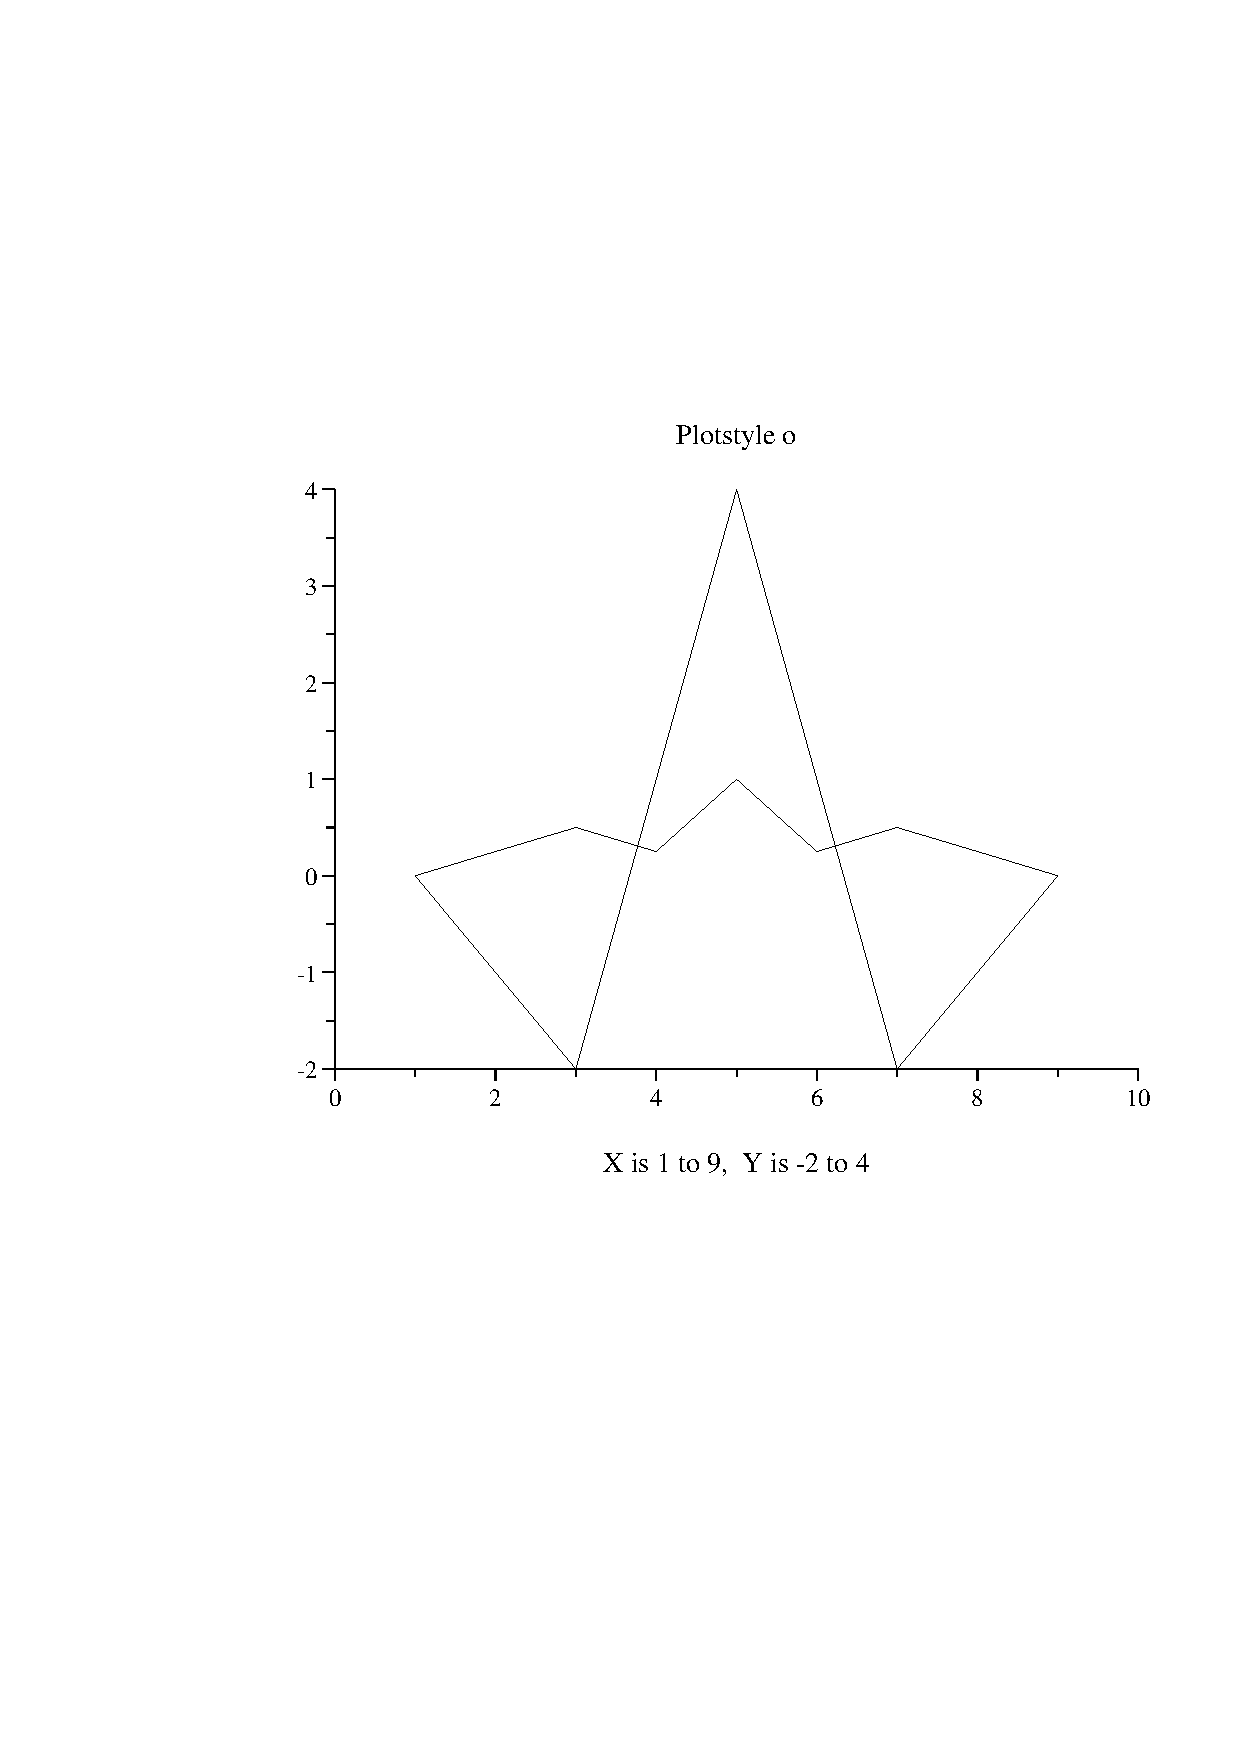
\epsfig{file=style-o,height=6.5cm}}
\end{center}

\begin{center}
\begin{boxedverbatim}

plt styles.data -p 0,1,2o -t "Plotstyle o"\end{boxedverbatim}

\end{center}
\end{figure}%
\lthtmlfigureZ
\lthtmlcheckvsize\clearpage}

{\newpage\clearpage
\lthtmlfigureA{figure1502}%
\begin{figure}\begin{center}
\fcolorbox{blue}{white}{
\epsfig{file=style-O,height=6.5cm}}
\end{center}

\begin{center}
\begin{boxedverbatim}

plt styles.data -p "0,1,2O(G.90)" -t "Plotstyle O"\end{boxedverbatim}

\end{center}
\end{figure}%
\lthtmlfigureZ
\lthtmlcheckvsize\clearpage}

{\newpage\clearpage
\lthtmlfigureA{figure1514}%
\begin{figure}\begin{center}
\fcolorbox{blue}{white}{
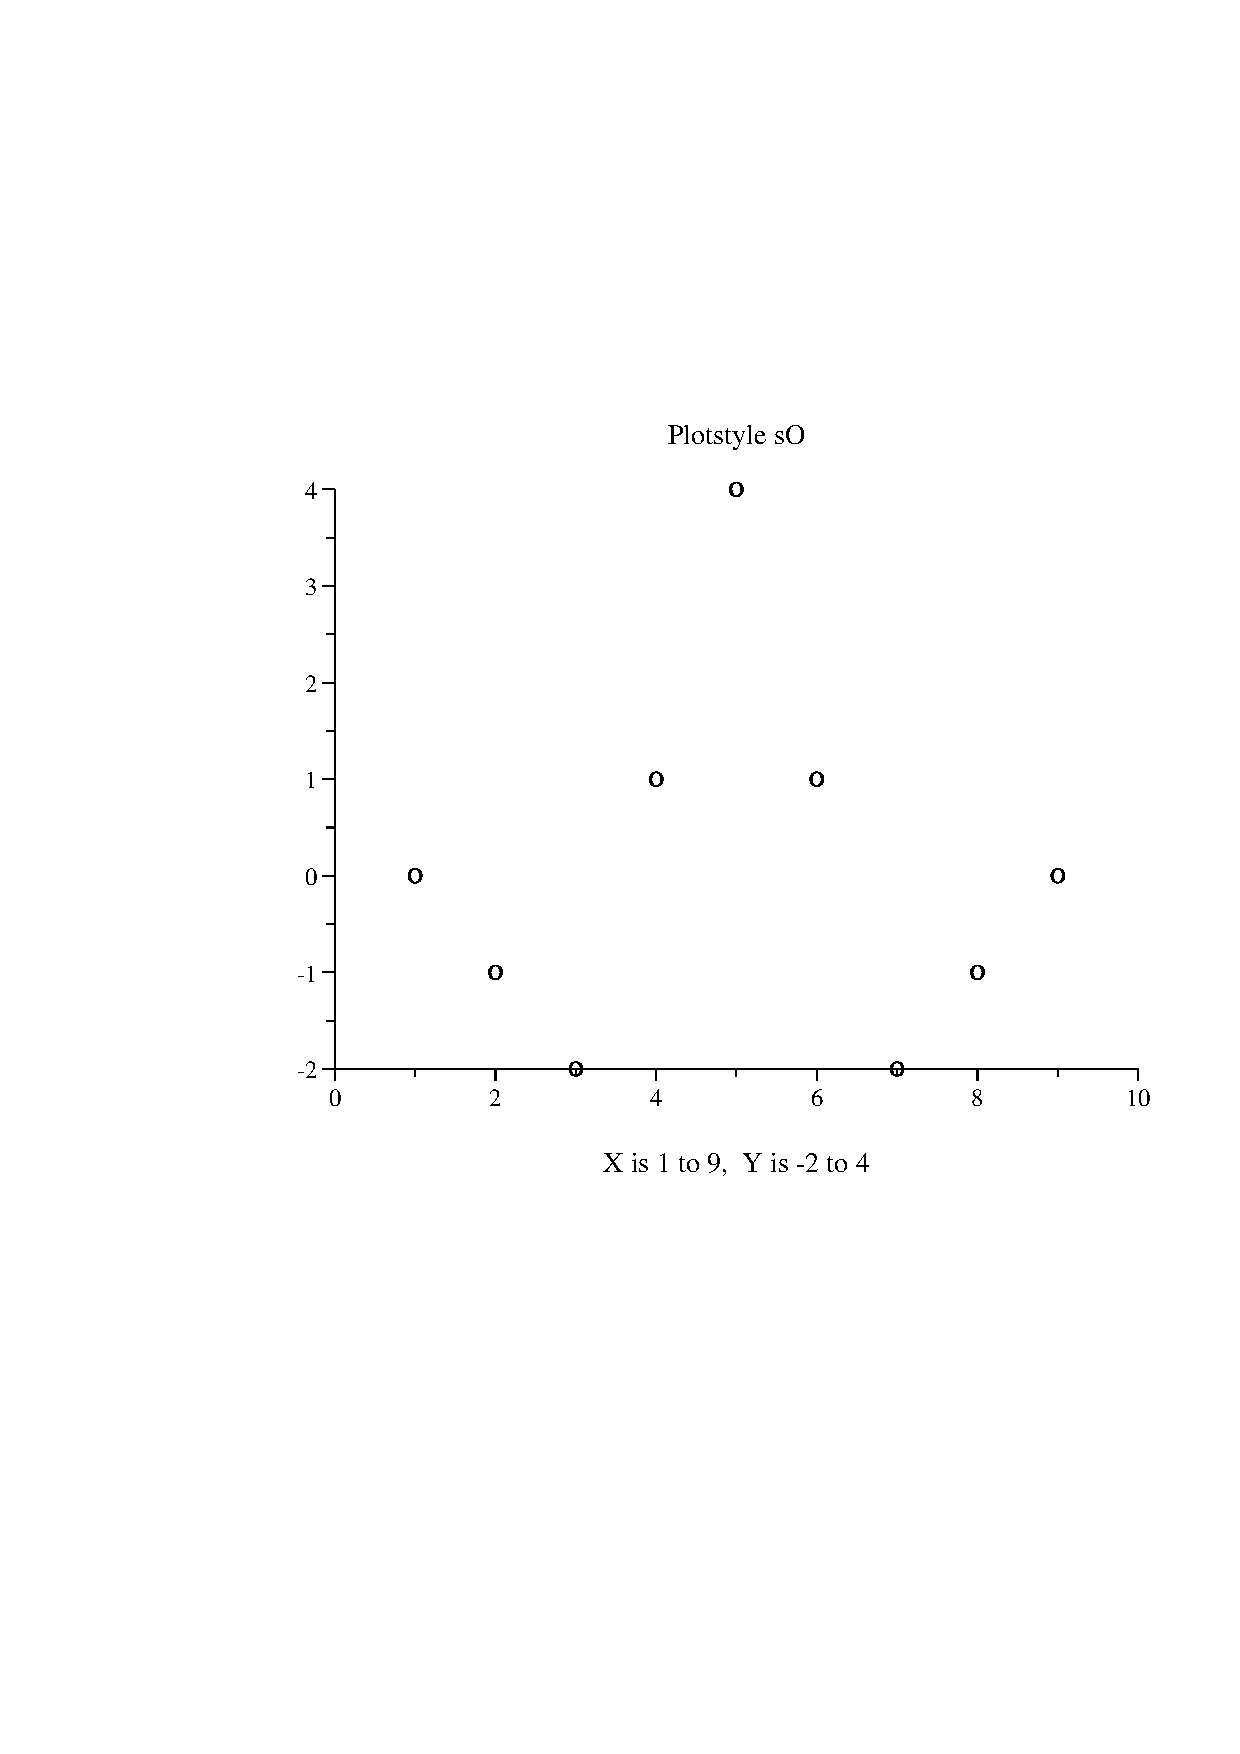
\epsfig{file=style-sO,height=6.5cm}}
\end{center}

\begin{center}
\begin{boxedverbatim}

plt styles.data -p 0,1sO -t "Plotstyle sO"\end{boxedverbatim}

\end{center}
\end{figure}%
\lthtmlfigureZ
\lthtmlcheckvsize\clearpage}

{\newpage\clearpage
\lthtmlfigureA{figure1526}%
\begin{figure}\begin{center}
\fcolorbox{blue}{white}{
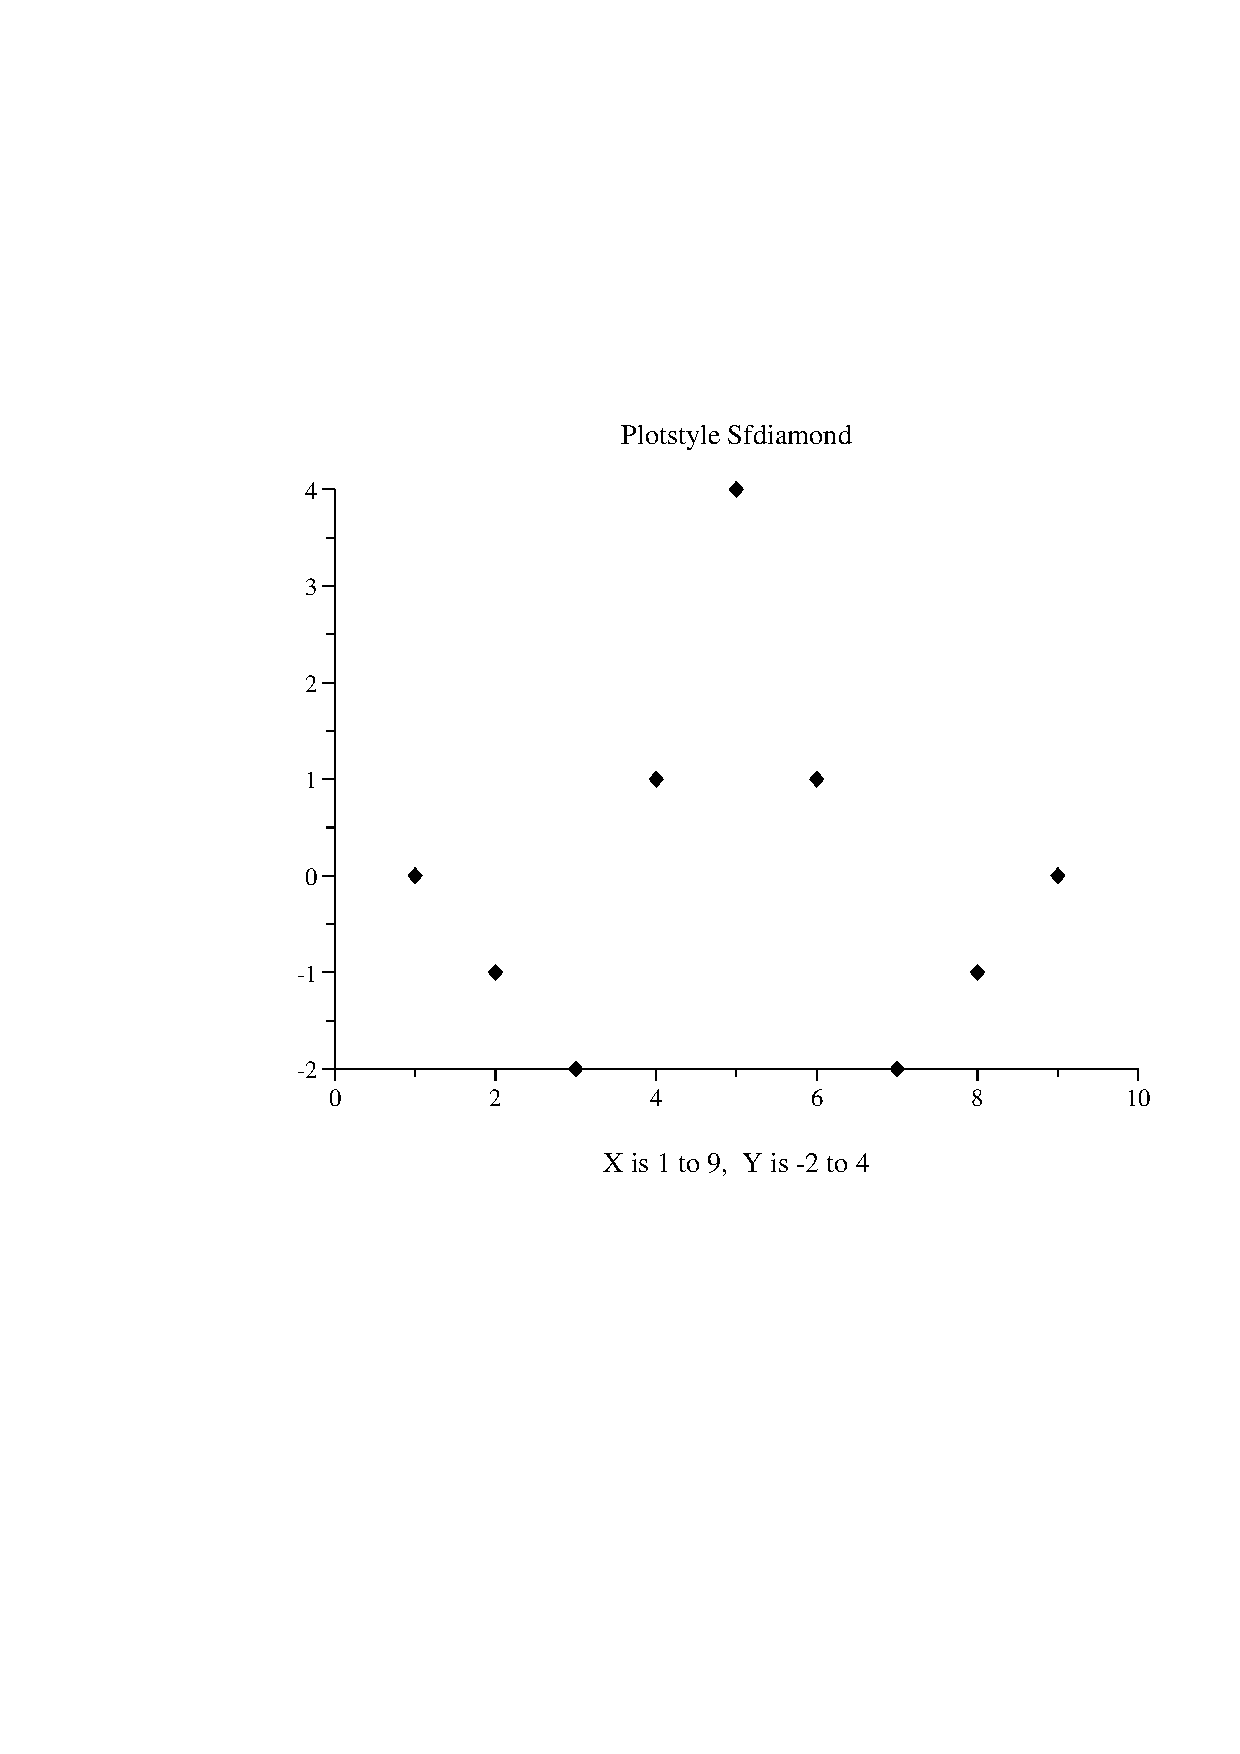
\epsfig{file=style-Sfdiamond,height=6.5cm}}
\end{center}

\begin{center}
\begin{boxedverbatim}

plt styles.data -p 0,1Sfdiamond -t "Plotstyle Sfdiamond"\end{boxedverbatim}

\end{center}
\end{figure}%
\lthtmlfigureZ
\lthtmlcheckvsize\clearpage}

{\newpage\clearpage
\lthtmlfigureA{figure1538}%
\begin{figure}\begin{center}
\fcolorbox{blue}{white}{
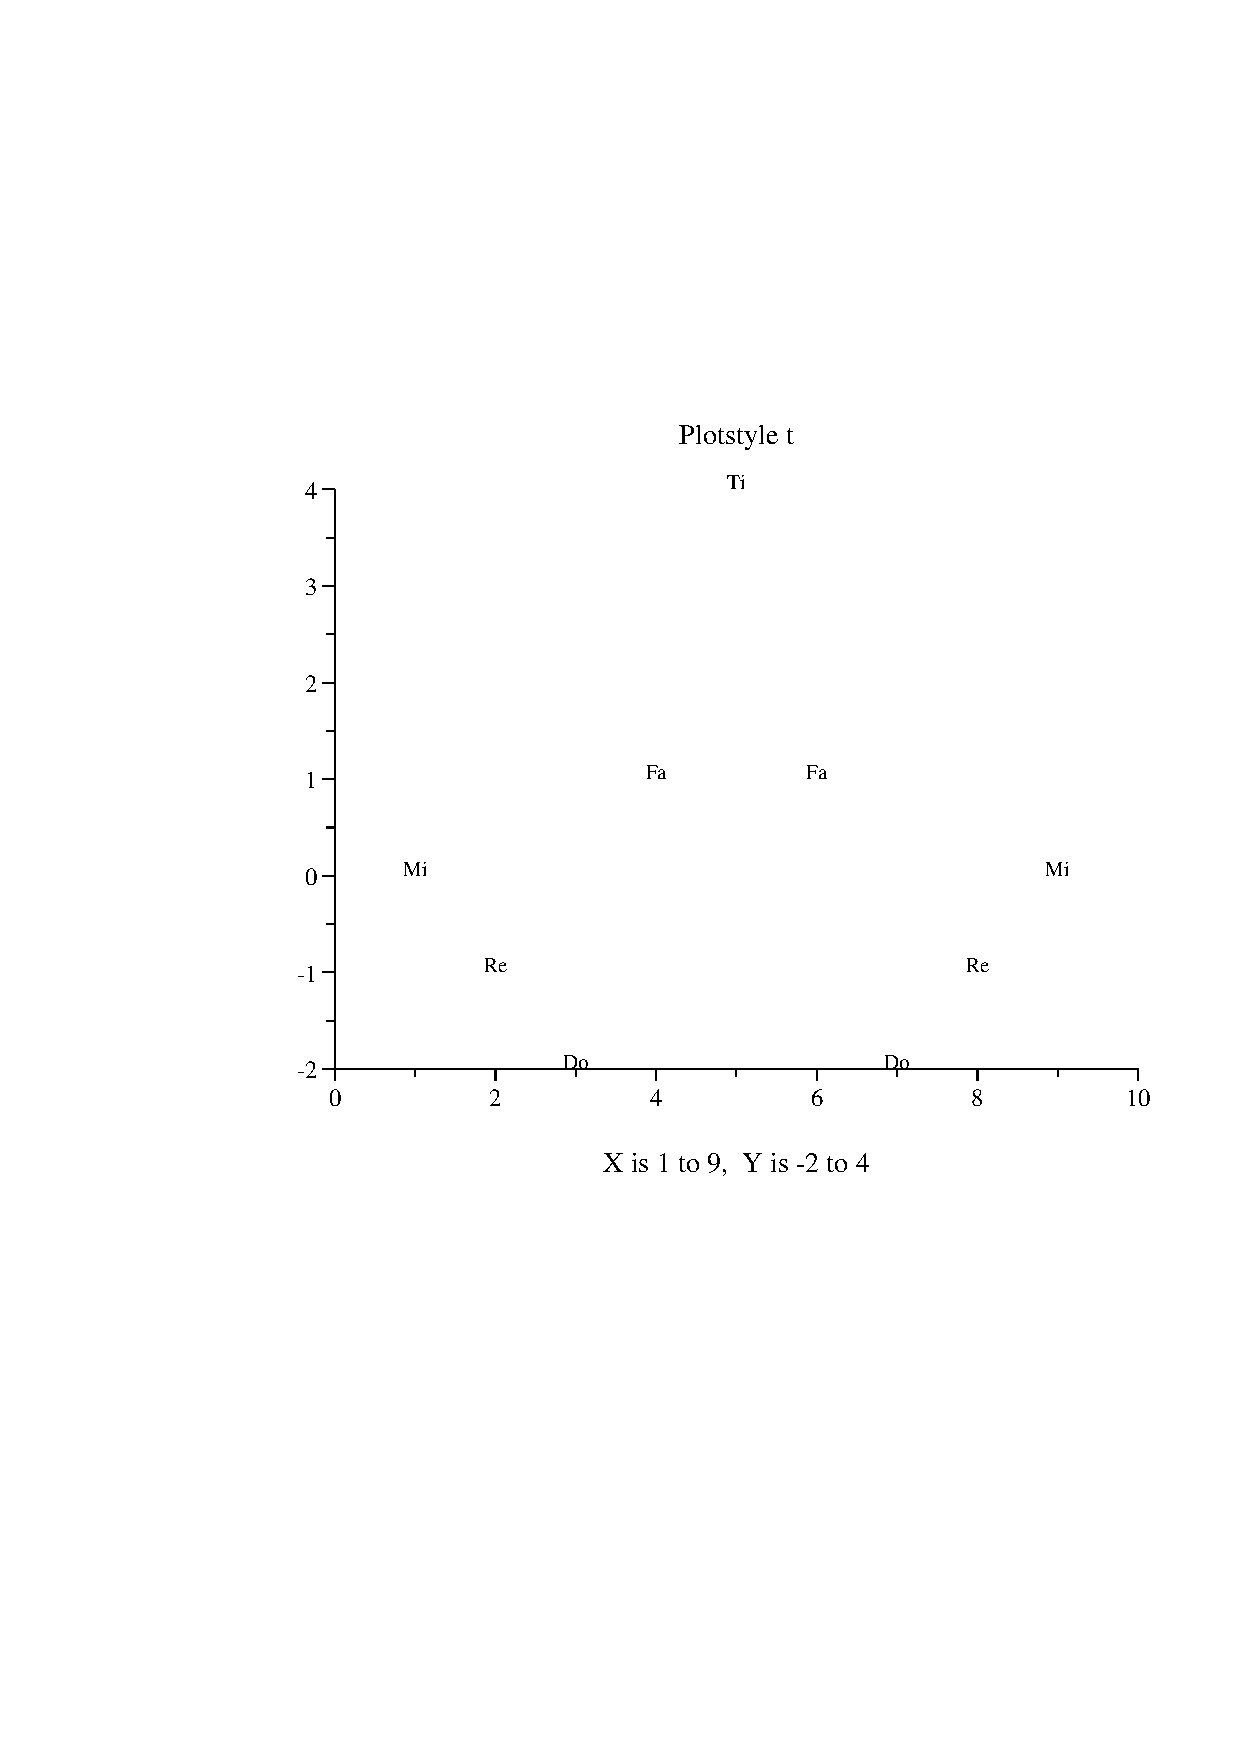
\epsfig{file=style-t,height=6.5cm}}
\end{center}

\begin{center}
\begin{boxedverbatim}

plt styles.data -p 0,1,3t -t "Plotstyle t" \
    -ts "Do Re Mi Fa Sol La Ti" CB\end{boxedverbatim}

\end{center}
\end{figure}%
\lthtmlfigureZ
\lthtmlcheckvsize\clearpage}

\stepcounter{chapter}
\stepcounter{section}
{\newpage\clearpage
\lthtmlfigureA{figure1556}%
\begin{figure}\begin{center}
\begin{tabular}{p{10cm}p{1.5cm}}
\fcolorbox{blue}{white}{
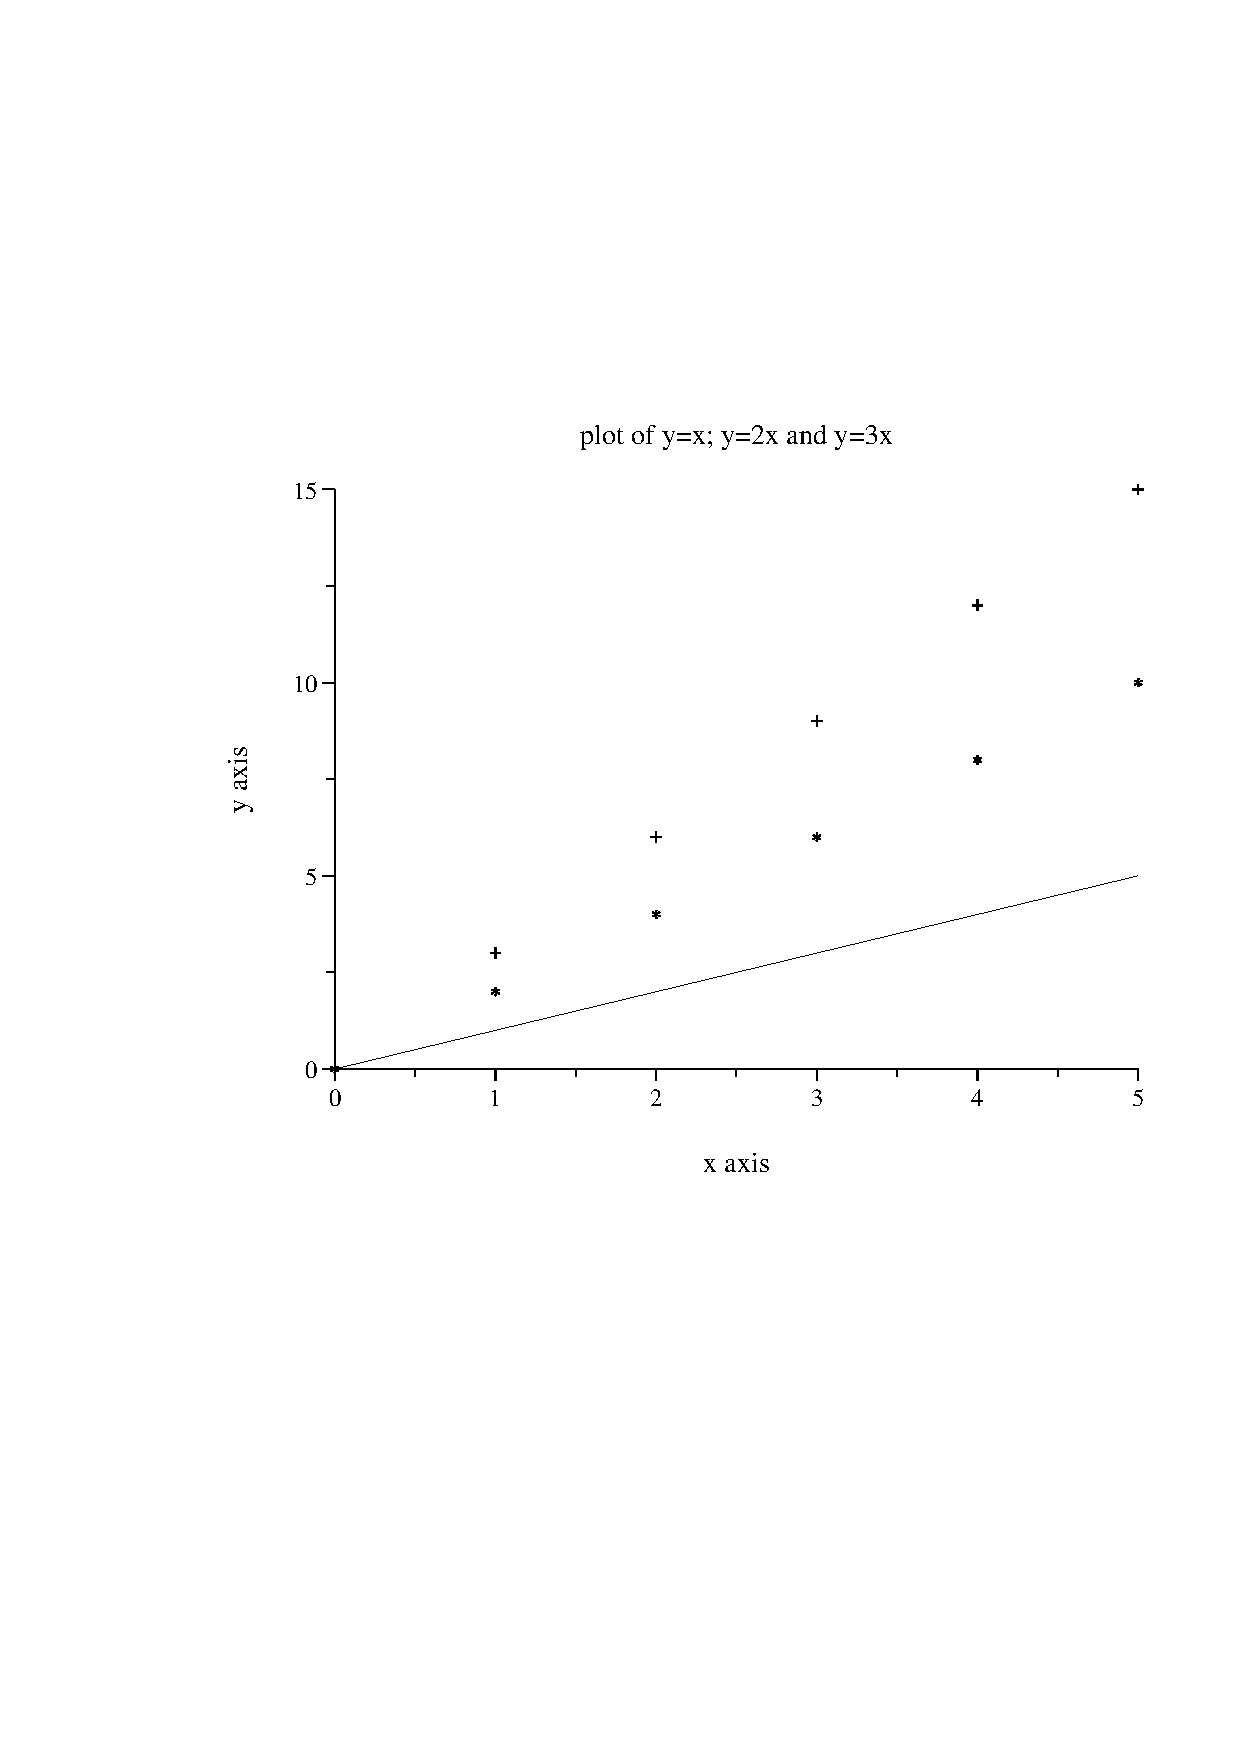
\epsfig{file=figure6,height=8cm}} &
{\vspace{-8cm}
{\em Data}
\vspace*{3mm}
\par
\begin{boxedverbatim}

0 0 0 0
1 1 2 3
2 2 4 6
3 3 6 9
4 4 8 12
5 5 10 15\end{boxedverbatim}

}
\end{tabular}
\end{center}

\begin{center}
\begin{boxedverbatim}

plt example5.data 0 3 0 2 1 -F"p s+ s* m"
    -x "x axis" -y "y axis" -t "plot of y=x; y=2x and y=3x"\end{boxedverbatim}

\end{center}
This command produces three traces on the same pair of axes (using
``{\tt +}'' to make a scatter plot of columns 0 and 3, ``{\tt *}'' to
make another scatter plot of columns 0 and 2, and using columns 0 and
1 to make a normal plot).
\end{figure}%
\lthtmlfigureZ
\lthtmlcheckvsize\clearpage}

{\newpage\clearpage
\lthtmlinlinemathA{tex2html_wrap_inline3881}%
$y = 5 x + 20$%
\lthtmlinlinemathZ
\lthtmlcheckvsize\clearpage}

{\newpage\clearpage
\lthtmlinlinemathA{tex2html_wrap_inline3883}%
$y = 2x^{2}$%
\lthtmlinlinemathZ
\lthtmlcheckvsize\clearpage}

{\newpage\clearpage
\lthtmlfigureA{figure1603}%
\begin{figure}\begin{center}
\begin{tabular}{p{10cm}p{1.5cm}}
\fcolorbox{blue}{white}{
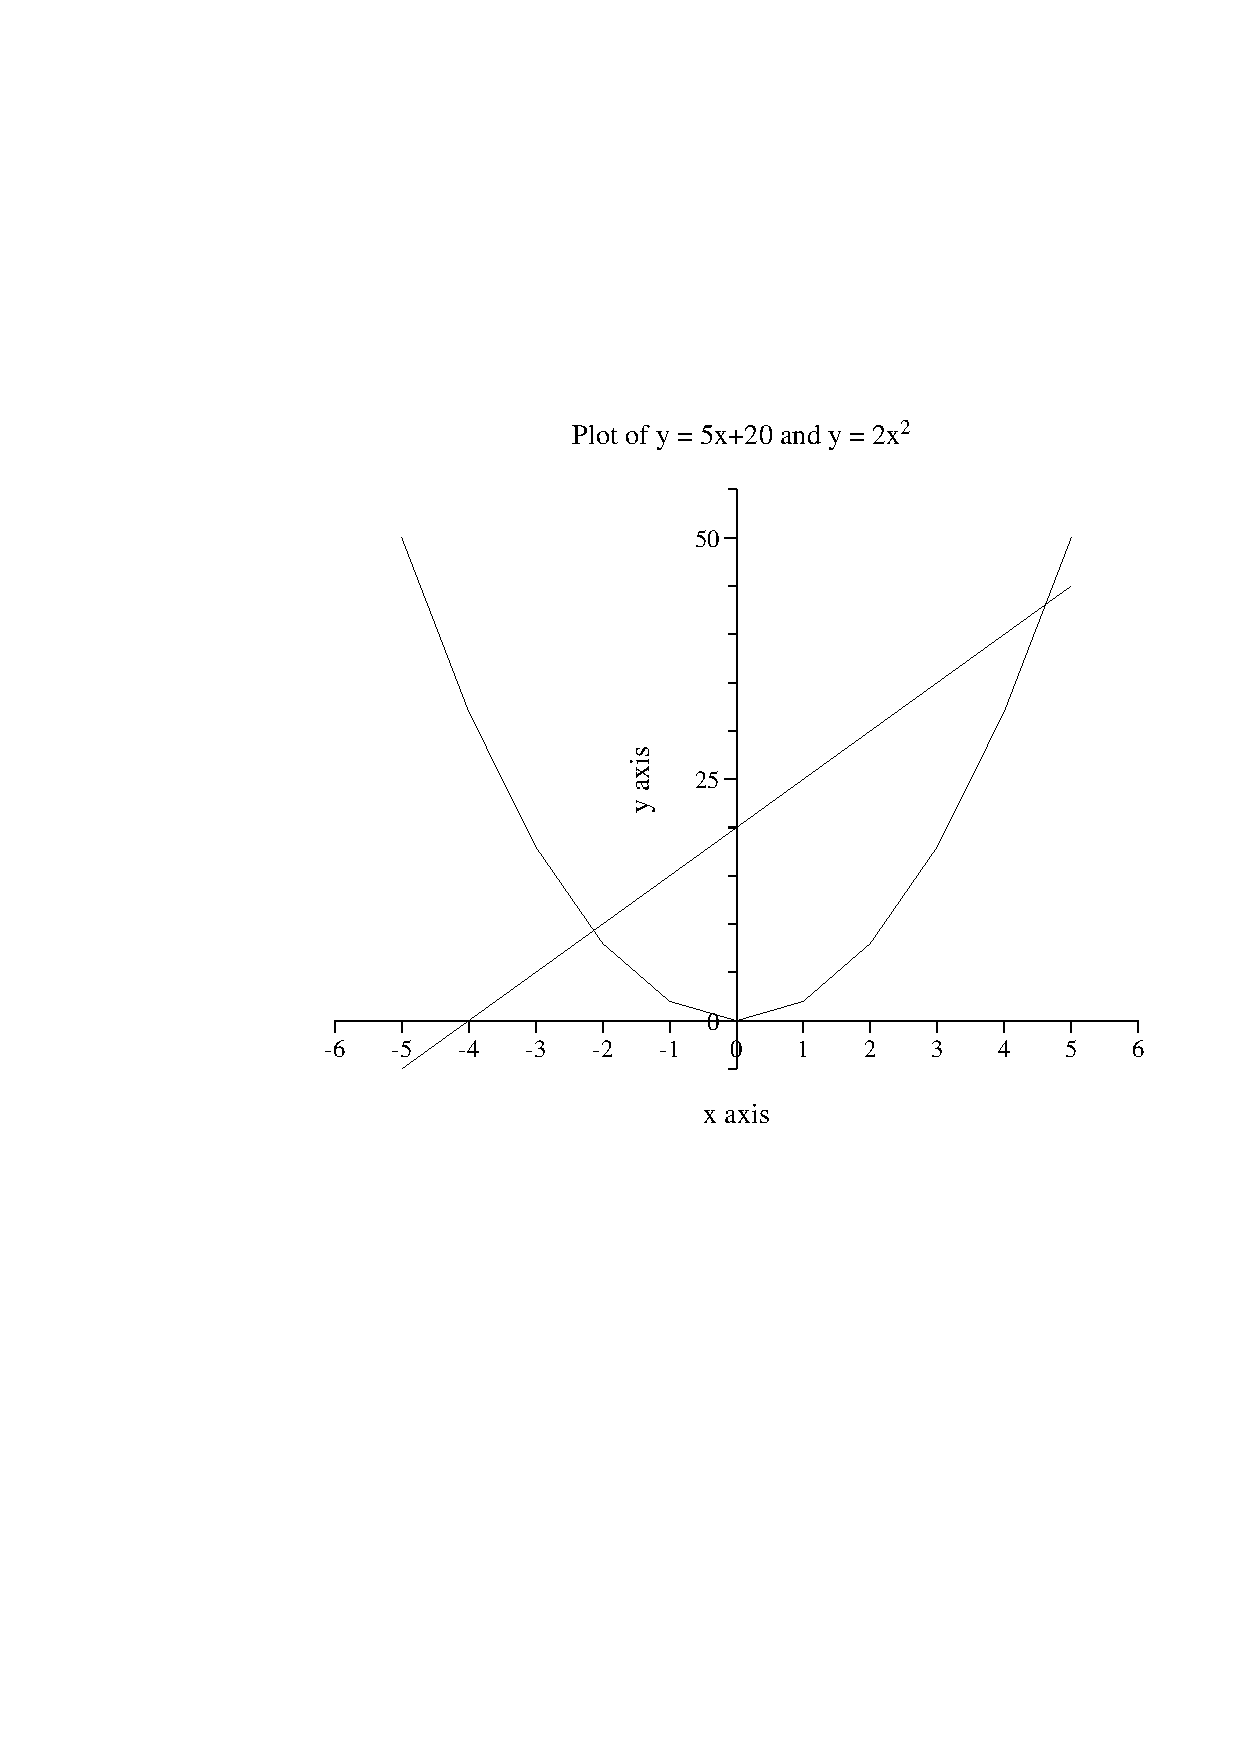
\epsfig{file=figure7,height=8cm}} &
{\vspace{-8cm}
{\em Data}
\vspace*{3mm}
\par
\begin{boxedverbatim}

-5 50 -5
-4 32 0
-3 18 5
-2 8 10
-1 2 15
0 0 20
1 2 25
2 8 30
3 18 35
4 32 40
5 50 45\end{boxedverbatim}

}
\end{tabular}
\end{center}

\end{figure}%
\lthtmlfigureZ
\lthtmlcheckvsize\clearpage}

\stepcounter{section}
{\newpage\clearpage
\lthtmlfigureA{figure1699}%
\begin{figure}\begin{center}
\fcolorbox{blue}{white}{
\epsfig{file=figure10,height=10cm}}
\end{center}

\end{figure}%
\lthtmlfigureZ
\lthtmlcheckvsize\clearpage}

\stepcounter{section}
{\newpage\clearpage
\lthtmlinlinemathA{tex2html_wrap_inline3887}%
$(xp0,yp0)$%
\lthtmlinlinemathZ
\lthtmlcheckvsize\clearpage}

{\newpage\clearpage
\lthtmlinlinemathA{tex2html_wrap_inline3889}%
$(xp1,yp1)$%
\lthtmlinlinemathZ
\lthtmlcheckvsize\clearpage}

{\newpage\clearpage
\lthtmlfigureA{figure1761}%
\begin{figure}\begin{center}
\fcolorbox{blue}{white}{
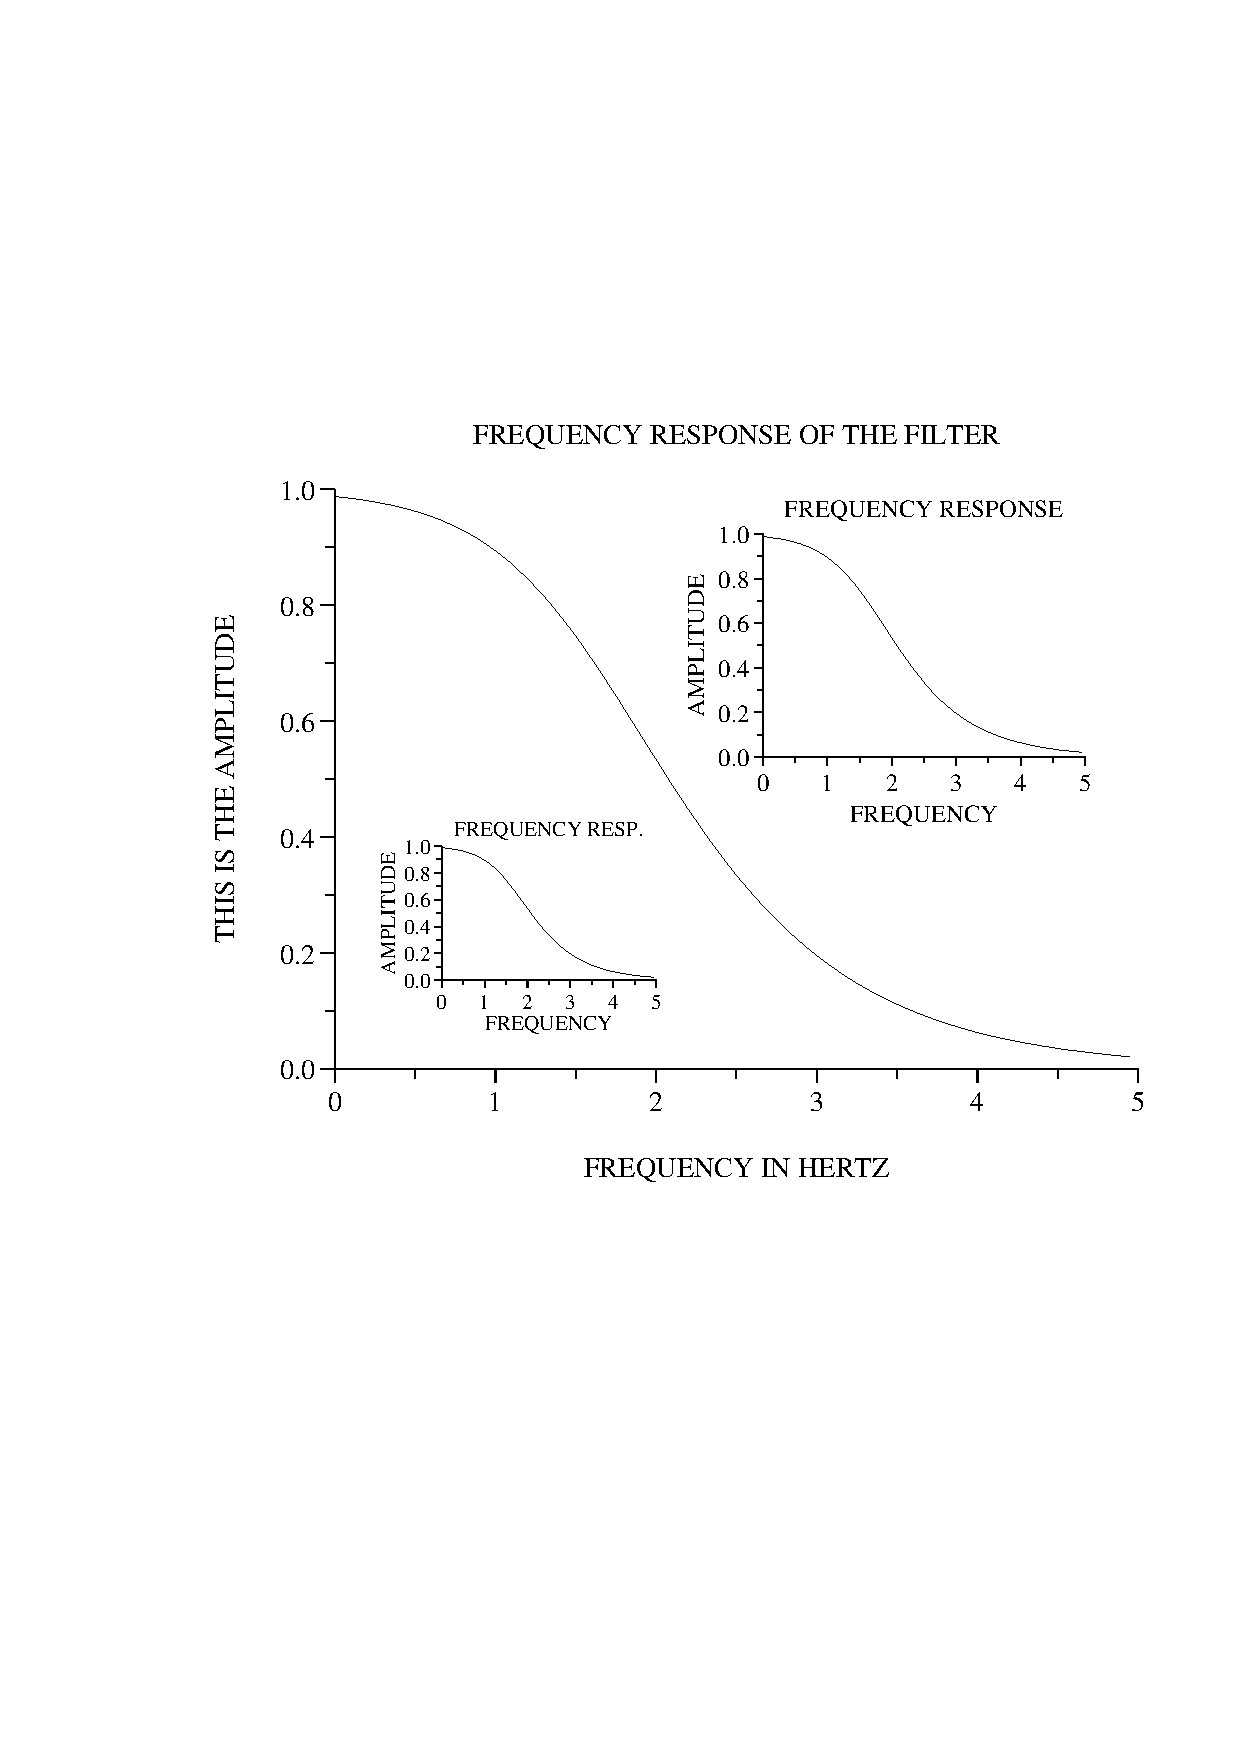
\epsfig{file=figure16,height=10cm}}
\end{center}

\begin{center}
\begin{boxedverbatim}

plt ldemo.data 2 3 -t"FREQUENCY RESPONSE OF THE FILTER" \
 -x"FREQUENCY IN HERTZ" -y"THIS IS THE AMPLITUDE" -sf all P16
plt ldemo.data 2 3 -t"FREQUENCY RESP." -x"FREQUENCY" \
 -y"AMPLITUDE"  -W .3 .3 .5 .45 -se -sf all P12
plt ldemo.data 2 3 -t"FREQUENCY RESPONSE" -x"FREQUENCY" \
 -y"AMPLITUDE"  -W .6 .55 .9 .8 -se -sf all P14\end{boxedverbatim}

\end{center}
\end{figure}%
\lthtmlfigureZ
\lthtmlcheckvsize\clearpage}

{\newpage\clearpage
\lthtmlfigureA{figure1793}%
\begin{figure}\begin{center}
\fcolorbox{blue}{white}{
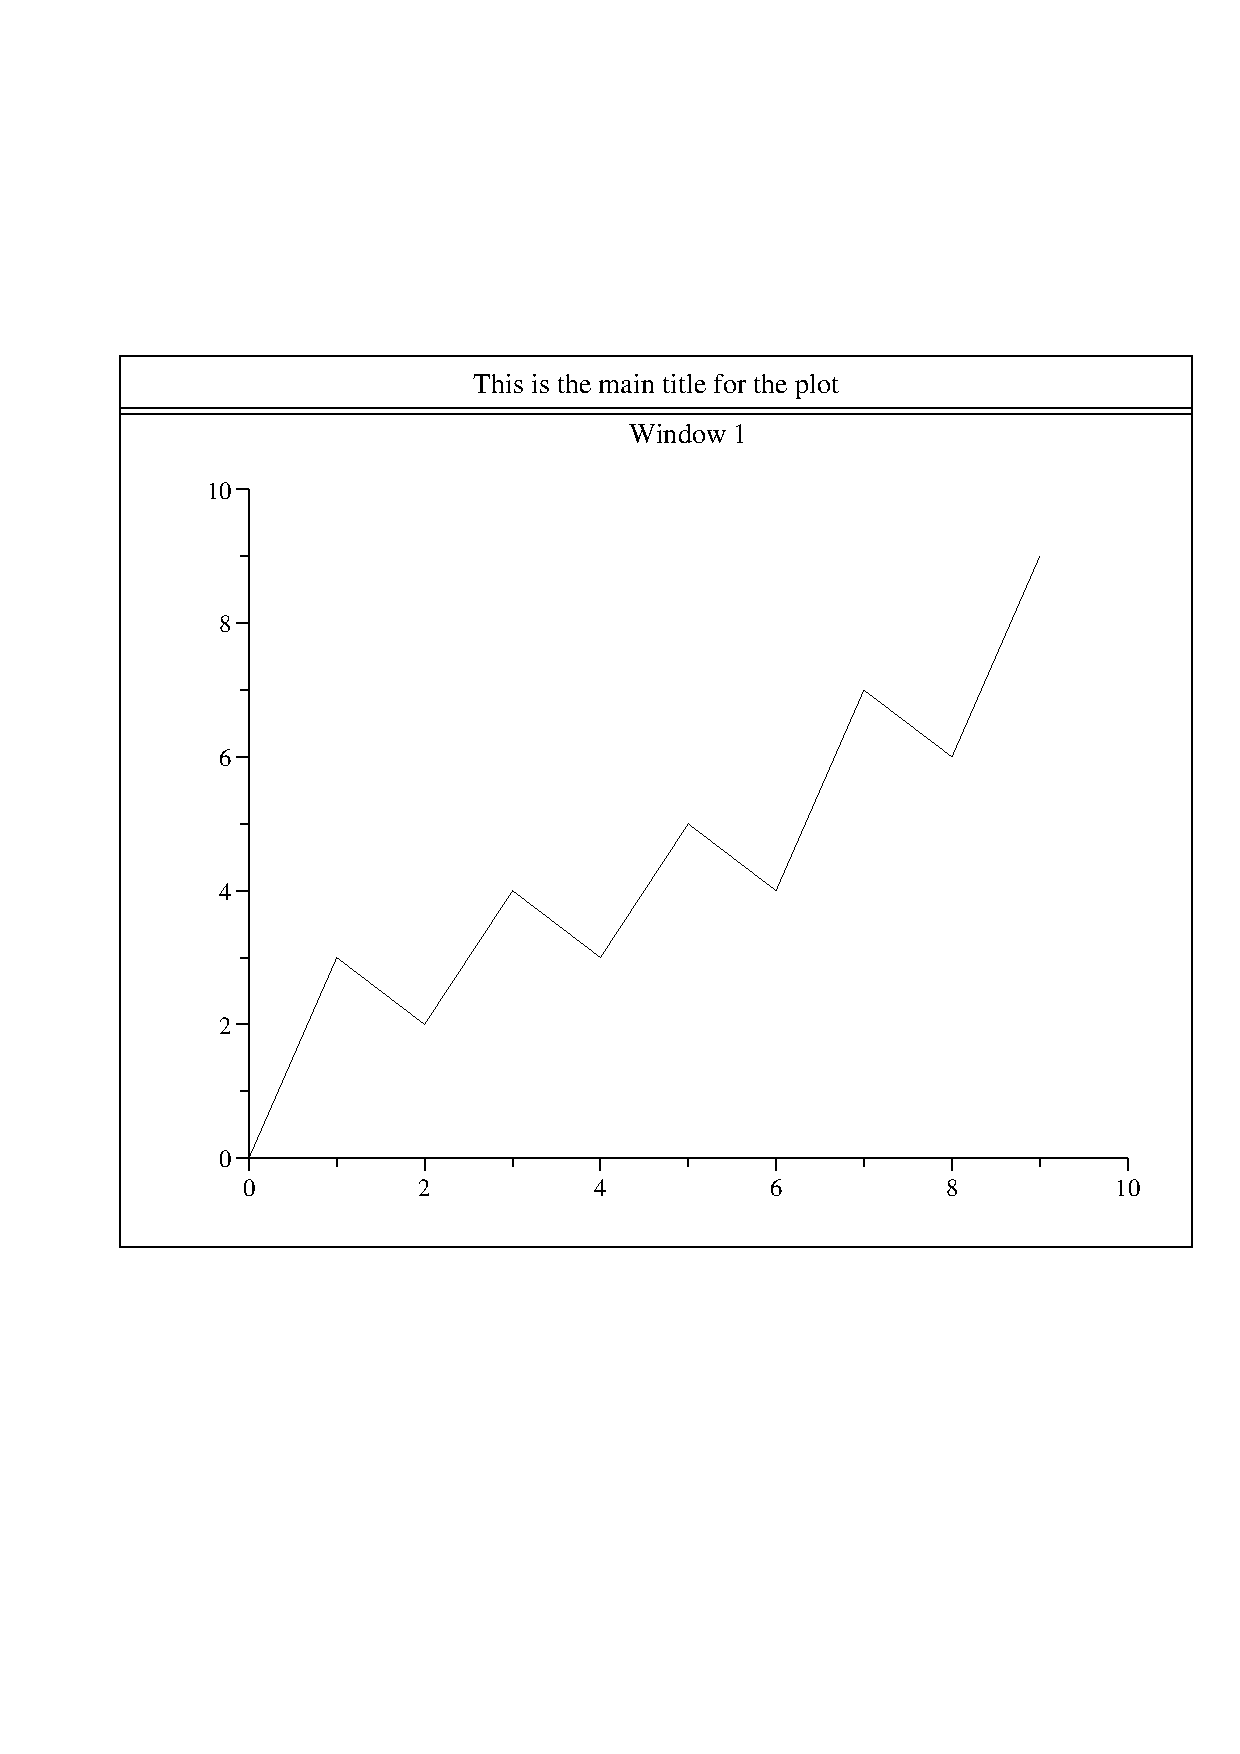
\epsfig{file=figure11,height=10cm}}

\par
\begin{boxedverbatim}

plt -wm 0 -t "This is the main title for the plot"
plt example11.data 0 1 -wm 1 -t "Window 1"\end{boxedverbatim}

\end{center}
\end{figure}%
\lthtmlfigureZ
\lthtmlcheckvsize\clearpage}

{\newpage\clearpage
\lthtmlfigureA{figure1803}%
\begin{figure}\begin{center}
\fcolorbox{blue}{white}{
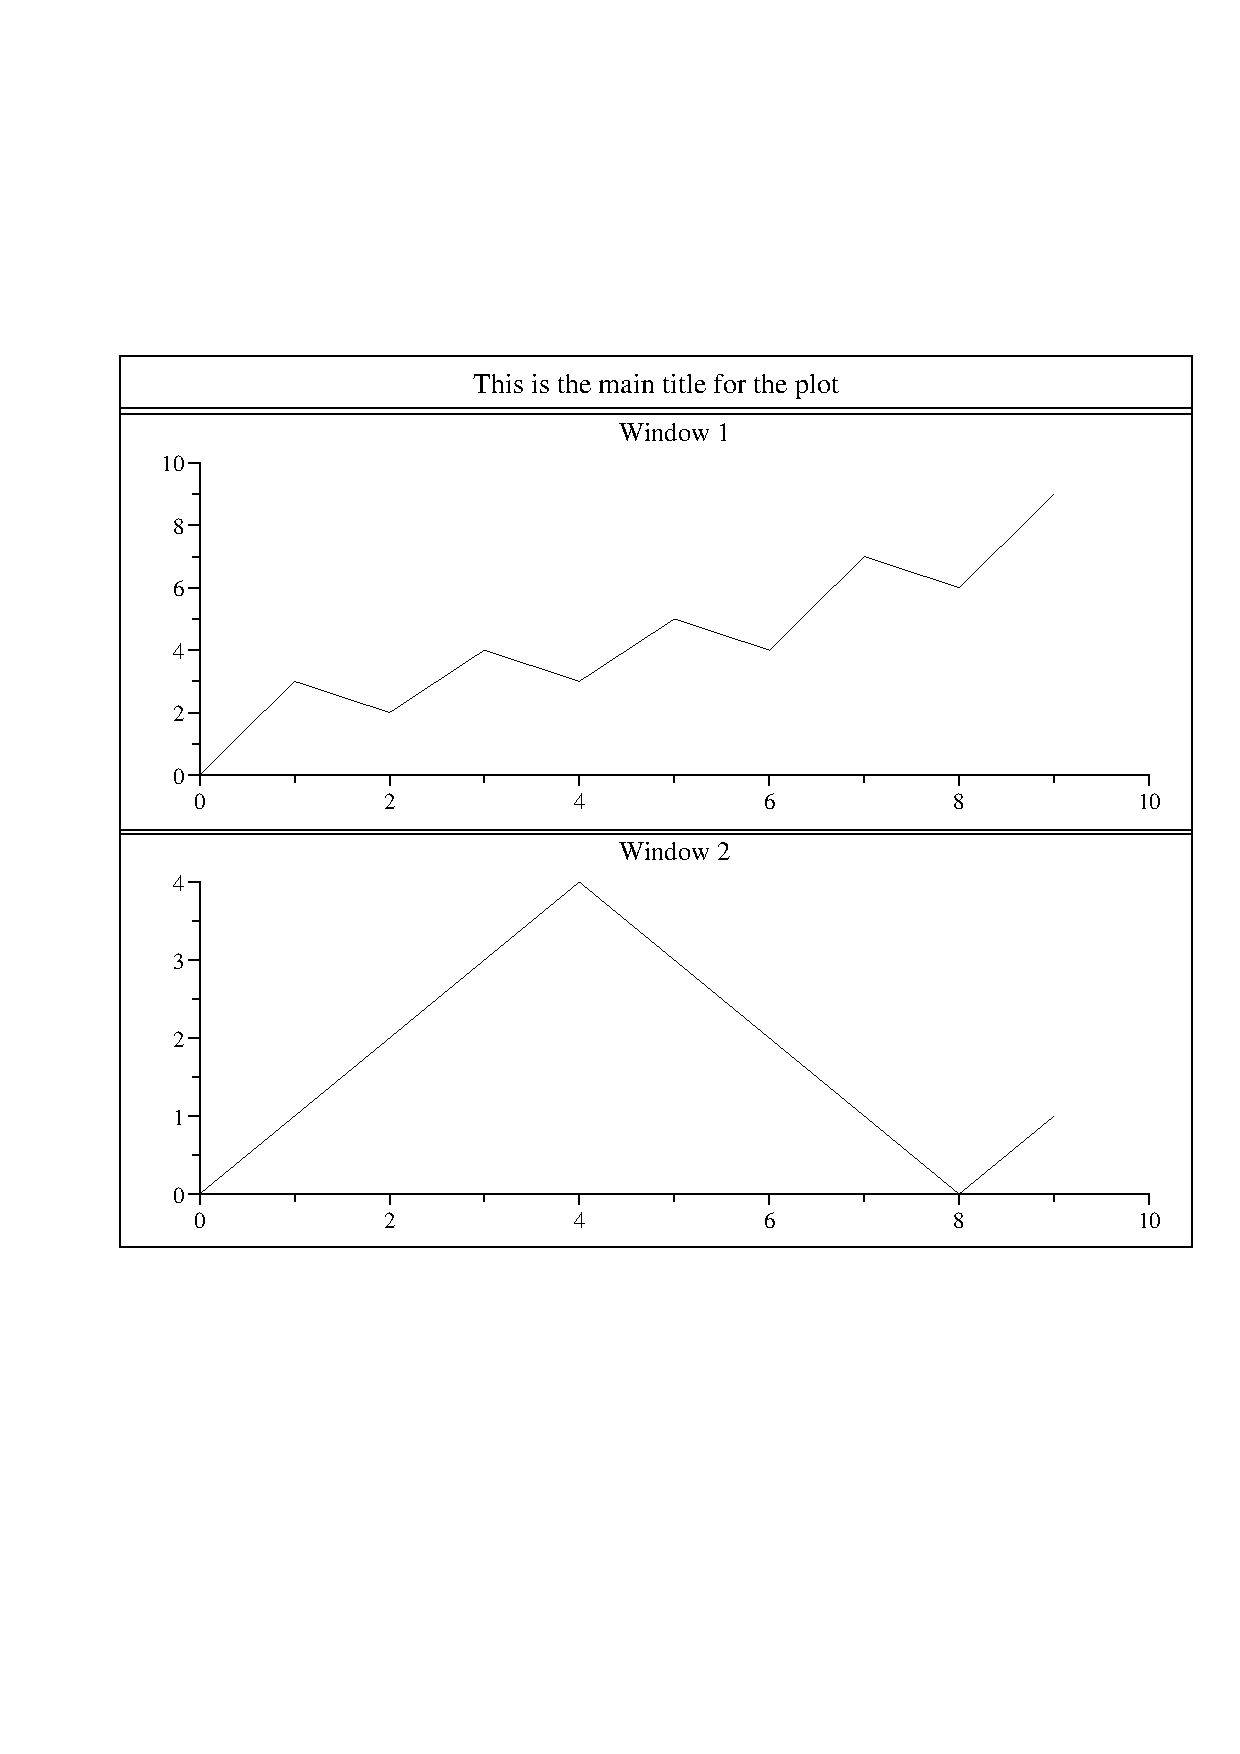
\epsfig{file=figure12,height=10cm}}

\par
\begin{boxedverbatim}

plt -wb 0 -t "This is the main title for the plot"
plt example11.data 0 1 -wb 1 -t "Window 1"
plt example11.data 0 2 -wb 2 -t "Window 2"\end{boxedverbatim}

\end{center}
\end{figure}%
\lthtmlfigureZ
\lthtmlcheckvsize\clearpage}

{\newpage\clearpage
\lthtmlfigureA{figure1813}%
\begin{figure}\begin{center}
\fcolorbox{blue}{white}{
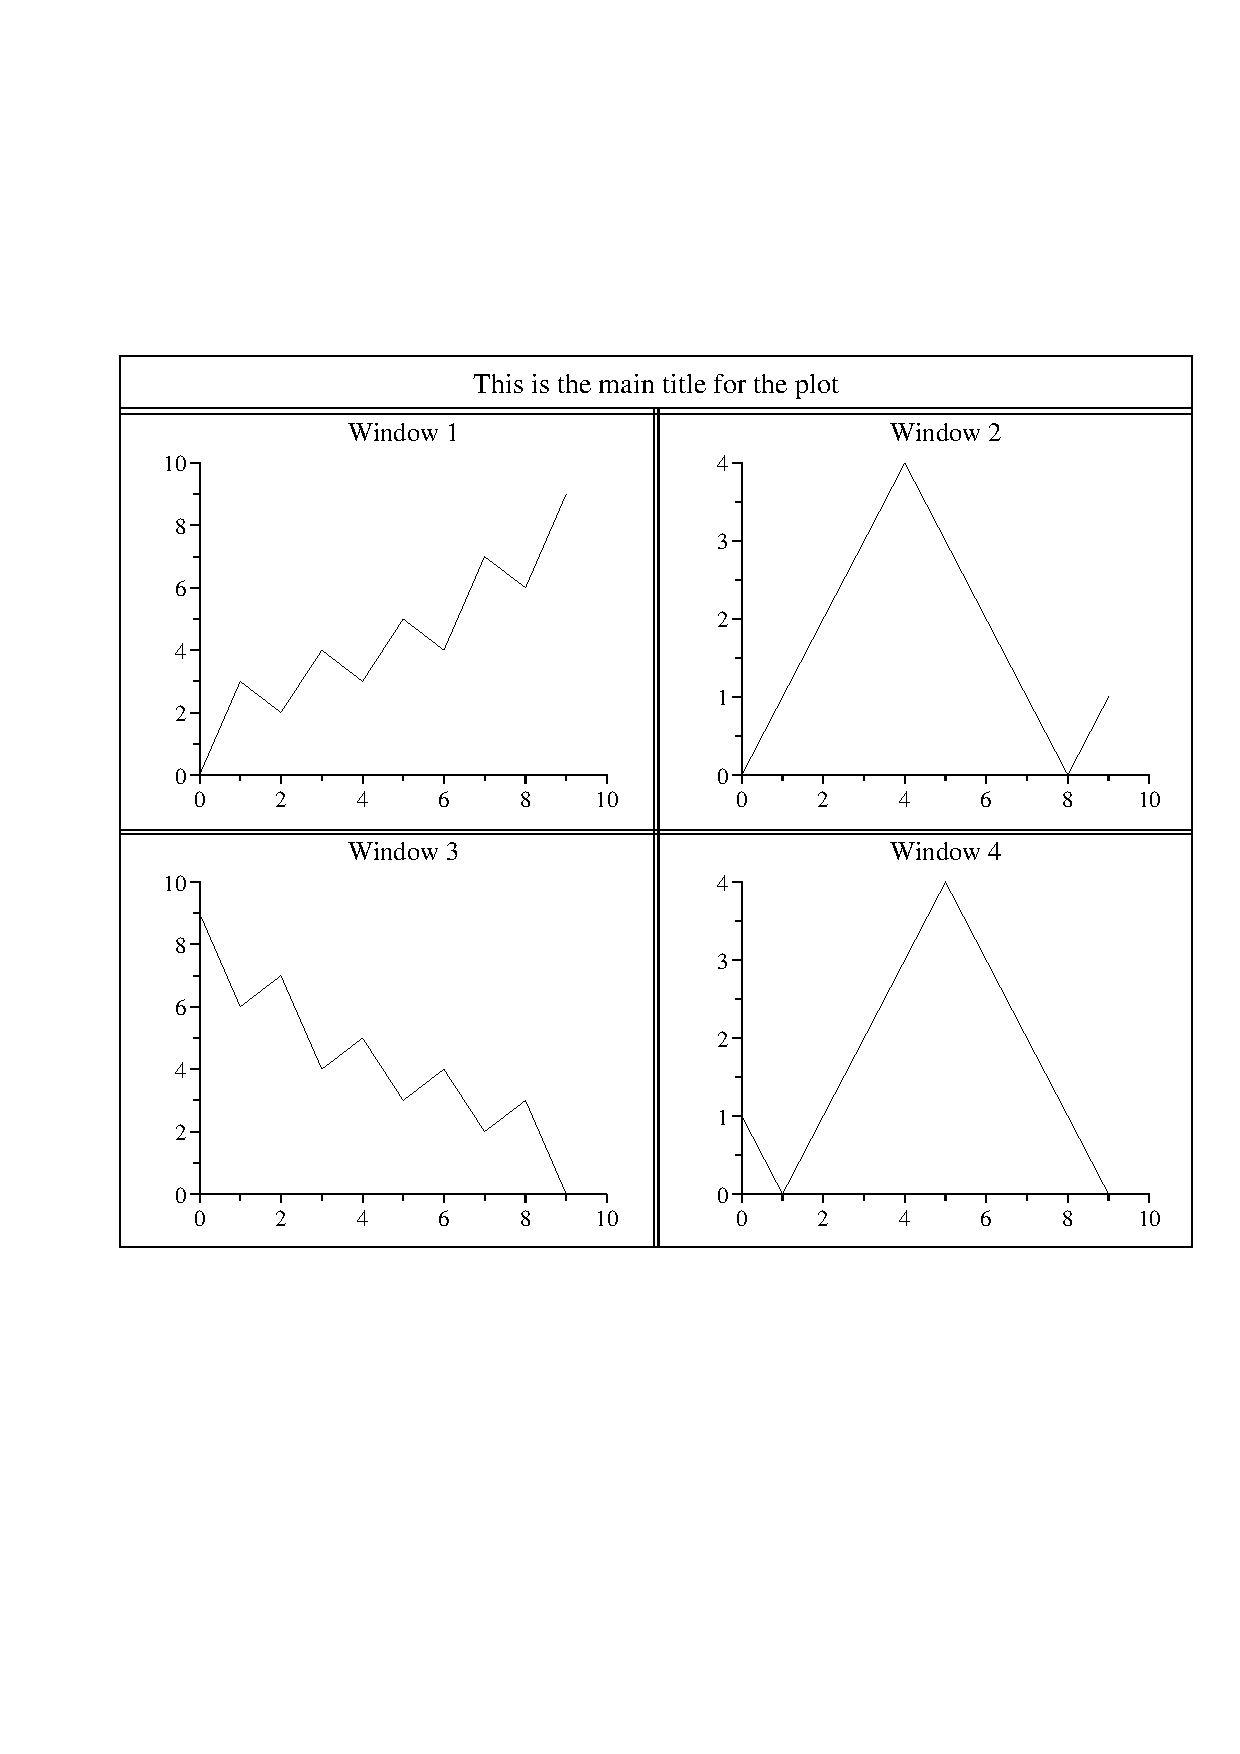
\epsfig{file=figure13,height=10cm}}

\par
\begin{boxedverbatim}

plt -wq 0 -t "This is the main title for the plot"
plt example11.data 0 1 -wq 1 -t "Window 1"
plt example11.data 0 2 -wq 2 -t "Window 2"
plt example11.data 0 3 -wq 3 -t "Window 3"
plt example11.data 0 4 -wq 4 -t "Window 4"\end{boxedverbatim}

\end{center}
\end{figure}%
\lthtmlfigureZ
\lthtmlcheckvsize\clearpage}

\stepcounter{chapter}
{\newpage\clearpage
\lthtmlinlinemathA{tex2html_wrap_inline3899}%
$xw$%
\lthtmlinlinemathZ
\lthtmlcheckvsize\clearpage}

{\newpage\clearpage
\lthtmlinlinemathA{tex2html_wrap_inline3901}%
$yw$%
\lthtmlinlinemathZ
\lthtmlcheckvsize\clearpage}

{\newpage\clearpage
\lthtmlfigureA{figure1894}%
\begin{figure}\begin{center}
\fcolorbox{blue}{white}{
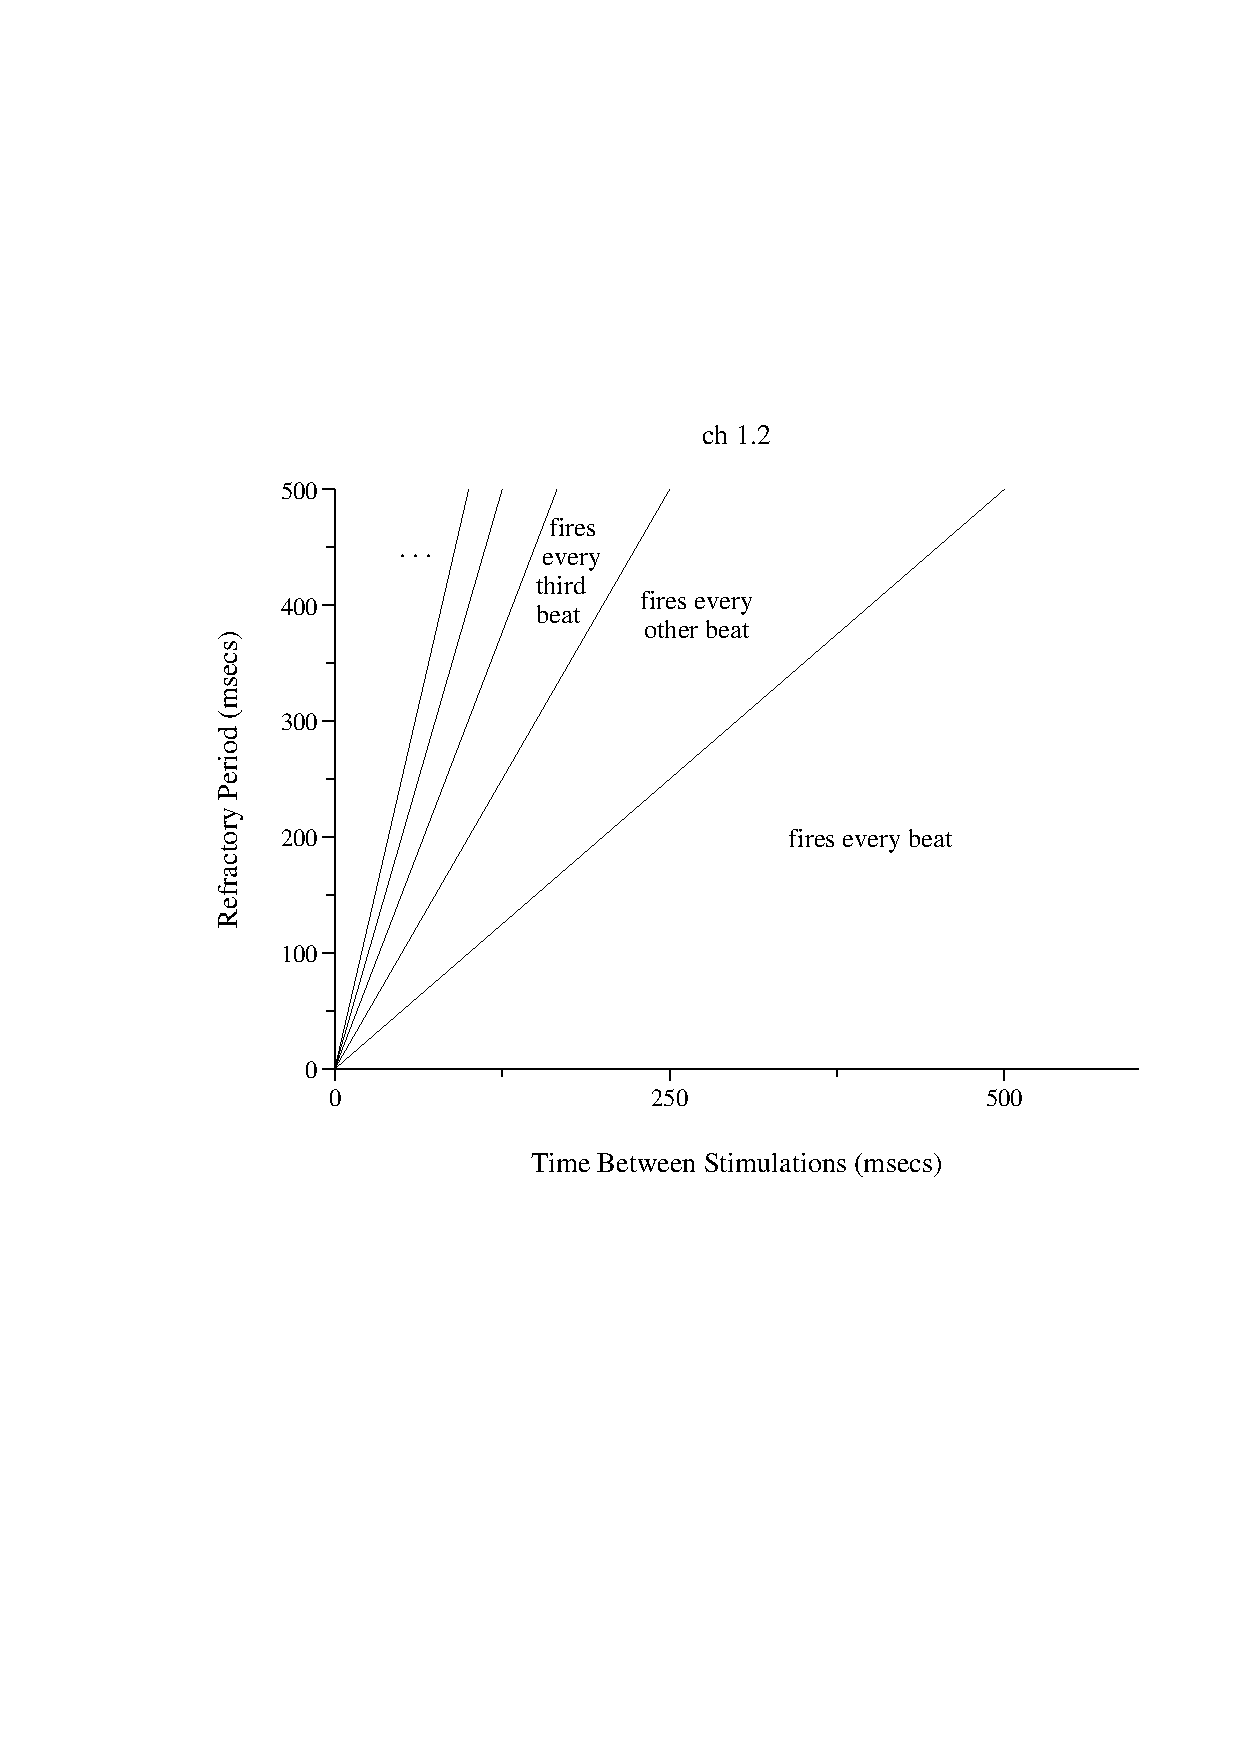
\epsfig{file=figure9,height=10cm}}
\end{center}

\begin{center}
\begin{boxedverbatim}

plt example9.data % -f example9.format
\end{boxedverbatim}

\end{center}
\end{figure}%
\lthtmlfigureZ
\lthtmlcheckvsize\clearpage}

\stepcounter{section}
{\newpage\clearpage
\lthtmlinlinemathA{tex2html_wrap_inline3913}%
$\mathrm{y = A\, sin ( \omega t + \phi )}$%
\lthtmlinlinemathZ
\lthtmlcheckvsize\clearpage}

{\newpage\clearpage
\lthtmlinlinemathA{tex2html_wrap_inline3915}%
$y = x^{\alpha} + x_{0}{\beta}$%
\lthtmlinlinemathZ
\lthtmlcheckvsize\clearpage}

{\newpage\clearpage
\lthtmlfigureA{figure1979}%
\begin{figure}\begin{center}
\fcolorbox{blue}{white}{
\epsfig{file=labels,height=8cm}}
\end{center}
%

\end{figure}%
\lthtmlfigureZ
\lthtmlcheckvsize\clearpage}

\stepcounter{chapter}
{\newpage\clearpage
\lthtmlinlinemathA{tex2html_wrap_inline3921}%
$(xw0,yw0)$%
\lthtmlinlinemathZ
\lthtmlcheckvsize\clearpage}

{\newpage\clearpage
\lthtmlinlinemathA{tex2html_wrap_inline3923}%
$(xw1,yw1)$%
\lthtmlinlinemathZ
\lthtmlcheckvsize\clearpage}

{\newpage\clearpage
\lthtmlinlinemathA{tex2html_wrap_inline3925}%
$(x0,y0)$%
\lthtmlinlinemathZ
\lthtmlcheckvsize\clearpage}

{\newpage\clearpage
\lthtmlinlinemathA{tex2html_wrap_inline3927}%
$(x1,y1)$%
\lthtmlinlinemathZ
\lthtmlcheckvsize\clearpage}

{\newpage\clearpage
\lthtmlfigureA{figure2069}%
\begin{figure}\begin{center}
\fcolorbox{blue}{white}{
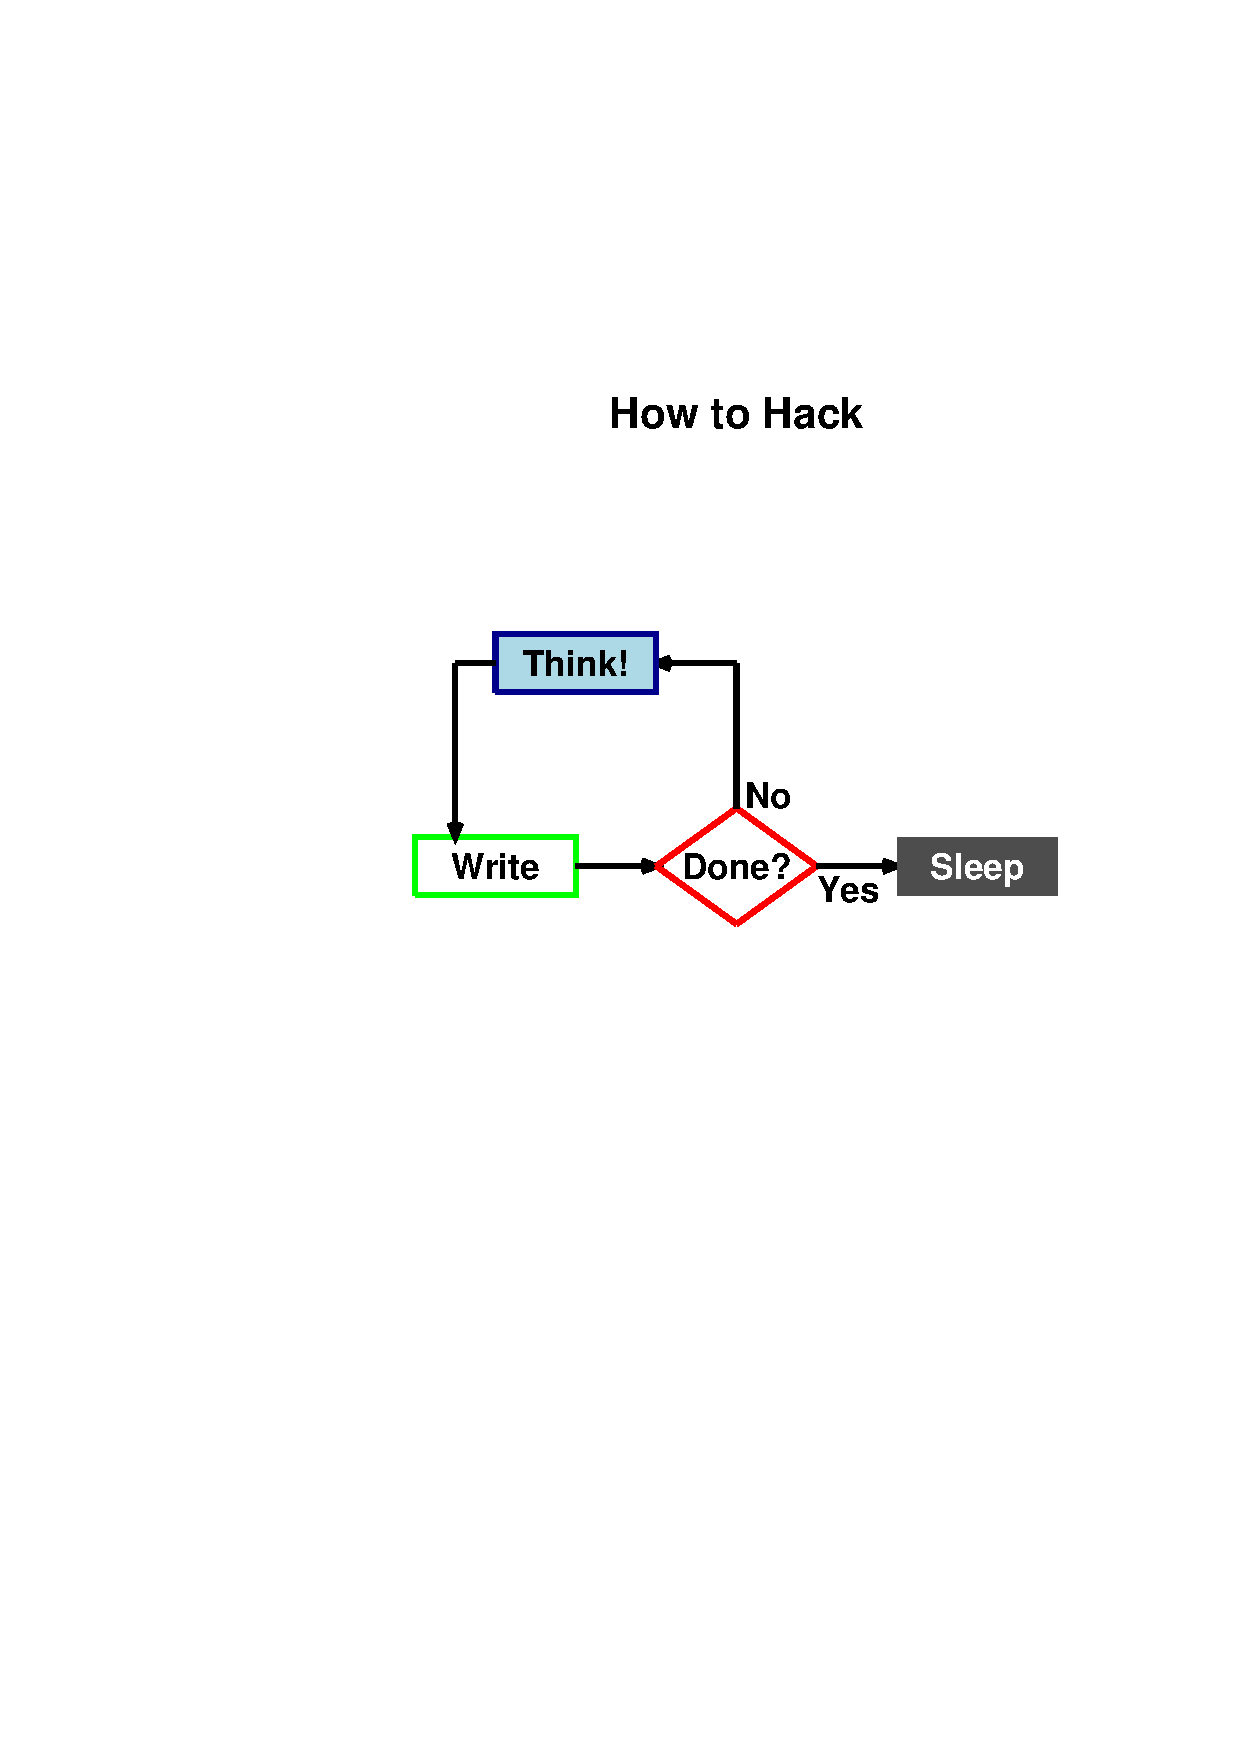
\epsfig{file=flowchart,height=10cm}}
\end{center}

\end{figure}%
\lthtmlfigureZ
\lthtmlcheckvsize\clearpage}

\stepcounter{chapter}
\stepcounter{chapter}
{\newpage\clearpage
\lthtmlfigureA{figure2237}%
\begin{figure}\begin{center}
\fcolorbox{blue}{white}{
\epsfig{file=fonts,height=10cm}}
\end{center}

\end{figure}%
\lthtmlfigureZ
\lthtmlcheckvsize\clearpage}

{\newpage\clearpage
\lthtmlfigureA{figure2245}%
\begin{figure}\begin{center}
\fcolorbox{blue}{white}{
\epsfig{file=linestyles,height=10cm}}
\end{center}

\end{figure}%
\lthtmlfigureZ
\lthtmlcheckvsize\clearpage}

{\newpage\clearpage
\lthtmlinlinemathA{tex2html_wrap_inline3939}%
$>N$%
\lthtmlinlinemathZ
\lthtmlcheckvsize\clearpage}

{\newpage\clearpage
\lthtmlfigureA{figure2311}%
\begin{figure}\begin{center}
\begin{tabular}{p{10cm}p{1.5cm}}
\fcolorbox{blue}{white}{
\epsfig{file=fontgroup1,height=8cm}} &
{\vspace{-85mm}\small {
{\em Data}
\vspace*{3mm}
\par
\begin{boxedverbatim}

0 0.034
5 0.771
10 1.003
15 0.464
20 -0.393
25 -1.005
30 -0.798
35 0.027
40 0.760
45 0.980
50 0.432
55 -0.421
60 -0.988
65 -0.780
70 0.045
75 0.823
80 0.988
85 0.456
90 -0.470
95 -0.964
100 -0.830\end{boxedverbatim}

}}
\end{tabular}
\end{center}

\end{figure}%
\lthtmlfigureZ
\lthtmlcheckvsize\clearpage}

{\newpage\clearpage
\lthtmlfigureA{figure2339}%
\begin{figure}\begin{center}
\fcolorbox{blue}{white}{
\epsfig{file=figure14,height=10cm}}
\end{center}

\end{figure}%
\lthtmlfigureZ
\lthtmlcheckvsize\clearpage}

{\newpage\clearpage
\lthtmlfigureA{figure2378}%
\begin{figure}\begin{center}
\fcolorbox{blue}{white}{
\epsfig{file=colors,height=10cm}}
\end{center}

\end{figure}%
\lthtmlfigureZ
\lthtmlcheckvsize\clearpage}

\stepcounter{chapter}
{\newpage\clearpage
\lthtmlinlinemathA{tex2html_wrap_inline3943}%
$e^0$%
\lthtmlinlinemathZ
\lthtmlcheckvsize\clearpage}

{\newpage\clearpage
\lthtmlinlinemathA{tex2html_wrap_inline3945}%
$e^1$%
\lthtmlinlinemathZ
\lthtmlcheckvsize\clearpage}

{\newpage\clearpage
\lthtmlinlinemathA{tex2html_wrap_inline3947}%
$e^2$%
\lthtmlinlinemathZ
\lthtmlcheckvsize\clearpage}

{\newpage\clearpage
\lthtmlfigureA{figure2486}%
\begin{figure}\begin{center}
\fcolorbox{blue}{white}{
\epsfig{file=figure17,height=10cm}}
\end{center}

\par
\begin{center}
\begin{boxedverbatim}

plt -wq 0 -t"THE TITLE FOR THE ENTIRE GRAPH GOES HERE"
plt ldemo.data 2 3 -wqs 1 -lx -g in -t"LPF: Log Freq & Ticks in"
plt ldemo.data 4 5 -wqs 4 -lx -ly -g both -t"LPF: Log Freq & Ampl"
plt ldemo.data 0 1 -wqs 3 -lx e -g out  -t"Alternate base & Ticks out"
plt ldemo.data 6 7 -wqs 2 -lx -ly - yes \
 -g grid,sym,out -t"Log axes with grid"\end{boxedverbatim}

\end{center}
\end{figure}%
\lthtmlfigureZ
\lthtmlcheckvsize\clearpage}

{\newpage\clearpage
\lthtmlfigureA{figure2514}%
\begin{figure}\begin{center}
\fcolorbox{blue}{white}{
\epsfig{file=conf,height=10cm}}
\end{center}

\end{figure}%
\lthtmlfigureZ
\lthtmlcheckvsize\clearpage}

\appendix
\stepcounter{chapter}
{\newpage\clearpage
\lthtmlinlinemathA{tex2html_wrap_inline3963}%
$rrggbb$%
\lthtmlinlinemathZ
\lthtmlcheckvsize\clearpage}

{\newpage\clearpage
\lthtmlinlinemathA{tex2html_wrap_inline3965}%
$rr$%
\lthtmlinlinemathZ
\lthtmlcheckvsize\clearpage}

{\newpage\clearpage
\lthtmlinlinemathA{tex2html_wrap_inline3967}%
$gg$%
\lthtmlinlinemathZ
\lthtmlcheckvsize\clearpage}

{\newpage\clearpage
\lthtmlinlinemathA{tex2html_wrap_inline3969}%
$bb$%
\lthtmlinlinemathZ
\lthtmlcheckvsize\clearpage}

\stepcounter{chapter}
\stepcounter{section}
\stepcounter{section}
{\newpage\clearpage
\lthtmlfigureA{figure2718}%
\begin{figure}\begin{center}
\fcolorbox{blue}{white}{
\epsfig{file=fig}}
.
\end{center}
\end{figure}%
\lthtmlfigureZ
\lthtmlcheckvsize\clearpage}

{\newpage\clearpage
\lthtmlfigureA{figure2739}%
\begin{figure}\begin{center}
\fcolorbox{blue}{white}{
\epsfig{file=fig,height=10cm}}
\end{center}

\end{figure}%
\lthtmlfigureZ
\lthtmlcheckvsize\clearpage}

{\newpage\clearpage
\lthtmlfigureA{figure2757}%
\begin{figure}\begin{center}
\fcolorbox{blue}{white}{
\epsfig{file=fig,height=8cm,width=12cm,angle=90}}
\end{center}

\end{figure}%
\lthtmlfigureZ
\lthtmlcheckvsize\clearpage}

\stepcounter{section}
{\newpage\clearpage
\lthtmlpictureA{tex2html_wrap7737}%
\epsfig{file=fig,height=6cm,bbllx=100,bblly=425,bburx=300,
        bbury=625,clip=}%
\lthtmlpictureZ
\lthtmlcheckvsize\clearpage}

\stepcounter{section}
\stepcounter{section}
\stepcounter{chapter}
\stepcounter{chapter}
{\newpage\clearpage
\lthtmlinlinemathA{tex2html_wrap_inline8003}%
\fbox{
{\tt xpltwin} {\tt -g} {\em width}{\tt x}{\em height}{\tt +-}{\em xoff}{\tt +-}{\em yoff}}%
\lthtmlinlinemathZ
\lthtmlcheckvsize\clearpage}

\stepcounter{chapter}
\stepcounter{chapter}
\stepcounter{section}
\stepcounter{section}
\stepcounter{section}
\stepcounter{chapter}
\stepcounter{section}
\stepcounter{chapter}
{\newpage\clearpage
\lthtmlinlinemathA{tex2html_wrap_inline8911}%
$|$%
\lthtmlinlinemathZ
\lthtmlcheckvsize\clearpage}

{\newpage\clearpage
\lthtmlinlinemathA{tex2html_wrap_inline9199}%
$\char94{}$%
\lthtmlinlinemathZ
\lthtmlcheckvsize\clearpage}


\end{document}
